\documentclass[a4paper, 10pt, openany]{book} 
\usepackage[utf8]{inputenc} %to manage special characters
\usepackage[T1]{fontenc} %to manage special characters
\usepackage{charter}
\usepackage[Bjarne]{fncychap} %fancy chapter style (many more available, like Sonny or Lenny etc.)
\usepackage{fancyhdr} %to customize the headers
\usepackage[lmargin=1.25in, rmargin=1.25in, tmargin=1.25in, bmargin=1.25in]{geometry} %sets the margins for the pages
\setcounter{tocdepth}{2} %table of contents number depth for subsections (2 = x.x.x)
\setcounter{secnumdepth}{4} %numbering depth for headers for subsections in the text(4 = x.x.x.x)
\usepackage{url} %to include urls
\usepackage{listings} %include this if you want to include code in the thesis
\usepackage{amsmath,amssymb} %mathematical package
\usepackage{siunitx} %includes SI-units
\usepackage[bf]{caption} %makes float captions bold
\usepackage{array, booktabs} %to make better tables
\usepackage{float} %to include floats
\usepackage[export]{adjustbox} %to adjust floats
%\usepackage{subfig} %to include subfigures
\usepackage{hyperref}
\usepackage{chngcntr} %will make it possible to change the counter for tables, figures etc. such as below
\counterwithin{figure}{chapter} %change counter for figures within sections (also possible to choose for each chapter
\counterwithin{table}{chapter} %change counter for tables within sections
\counterwithin{section}{chapter}
\counterwithin{subsection}{section}
\usepackage{color, xcolor} %edit e.g. text colors
\usepackage{graphicx}
\usepackage{subcaption}
\usepackage[export]{adjustbox}
\usepackage{wrapfig}
\usepackage{caption}

%nikkis additions
\usepackage{blindtext} %latin filler text
\usepackage{multicol} %multiple columns
% Load the parskip package without options
\usepackage{parskip}
% Load the setspace package
\usepackage{setspace}
% graphics folder
\graphicspath{ {./images/}}
\setlength{\parskip}{1\baselineskip} %change the spacing between paragraphs
\usepackage{booktabs}
\usepackage{lscape}
\usepackage{rotating}
\usepackage{changepage} % Required for adjustwidth environment
\usepackage{tablefootnote} % for table footnotes
\usepackage[marginal]{footmisc}
\usepackage{CJKutf8} %for japanese
\usepackage[font=small]{caption} %make captions smaller
\usepackage[amsmath]

\ChNameVar{\fontsize{14}{22}\usefont{T1}{bch}{el}{n}\selectfont}
\ChNumVar{\fontsize{14}{22}\usefont{T1}{bch}{el}{n}\selectfont}
\ChTitleVar{\fontsize{14}{22}\usefont{T1}{phv}{b}{n}\selectfont}

\usepackage{titlesec}
\titleformat{\section}{\normalsize\bfseries}{\thesection}{1em}{}
\titlespacing*{\section}{0pt}{\parskip}{\parskip}
\titleformat{\subsection}{\normalsize}{\thesubsection}{1em}{}
\titlespacing*{\subsection}{0pt}{\parskip}{\parskip}

\usepackage[backend = biber,
            style = numeric,
            date = long,     % Long: 24th Mar. 1997 | Short: 24/03/1997
            sorting = none,
            maxcitenames = 3,   % max names to include before et. al.
            ]{biblatex} %customize the look of your citations and bibliography
\DeclareNameAlias{author}{last-first}
\addbibresource{references.bib} %Zotero bibliography file
\usepackage{comment} %to be able to comment out sections in the .tex files
\usepackage{afterpage} %to customize page commands such as below
\newcommand\myemptypage{
    \null
    \thispagestyle{empty}
    \addtocounter{page}{-1}
    \newpage
    } %sets new page command to insert an empty page without adding to the page counter or having a page number

\usepackage[titles]{tocloft}
\setlength{\cftfignumwidth}{4em}
\setlength{\cfttabnumwidth}{4em}

\begin{document}
%%%%%%%%%%%%%%%%%%%%%%%%%%%%%%%%%%%%%%%%%%%%%%%%%%%%%%%%
%\begin{comment}
%the title page should be an odd page (right hand side)

\begin{titlepage}
\newgeometry{left=1.5in, right=1.5in}
\vspace*{1.5cm}

\noindent{\large Nikki Hall} \\
\vspace{1cm}

\begin{doublespace}
\noindent
\textbf{\large Evaluating social gathering opportunities in a pandemic}\\
\textbf{\large through image classification and reach analysis of city parks}\\
%\vspace{0.25cm}

\begin{CJK}{UTF8}{min}
\noindent{\large 画像分類と到達圏解析を用いたパンデミック時の都市公園} \\
\noindent{\large におけるsocial gatheringの評価} \\\vspace{0.25cm}
\end{CJK}
\end{doublespace}

\vspace{6cm}
\noindent Master's thesis in Architecture and Urban Design \\
Supervisor: HONMA Kentaro \\
%Co-supervisor: Co-supervisor Name \\
July 2023 \\

\vspace{0.2cm}
\noindent University of Tokyo \\
School of Engineering \\
Department of Architecture \\

%\begin{figure}[h]
%    \includegraphics[width=0.28\textwidth]{Figures/ntnu_basic.png}
%\end{figure}
\end{titlepage}
\restoregeometry
\myemptypage %empty page such that the abstract starts at the first right hand side after the title page
%\end{comment}
%%%%%%%%%%%%%%%%%%%%%%%%%%%%%%%%%%%%%%%%%%%%%%%%%%%%%%%%

% The pre-chapters
\chapter*{Abstract} %pre-chapters should not be numbered, hence the "*"
\pagenumbering{roman} %introductory pages should be roman
\setcounter{page}{1}
\addcontentsline{toc}{chapter}{\protect\numberline{}Abstract} %add the chapter to the table of contents, this is not automatically added when creating unnumbered chapters (*). Add it in a chapter style, and keep all chapters on the same numberline indent regardless of number or not on the chapter
\noindent The challenges faced by the urban environment during the recent pandemic must be studied in order to be prepared for the next global health crisis. During the first weeks of the COVID-19 pandemic, cities around the world instituted stay-at-home orders and lockdowns of varying degrees, forcing their residents to adapt by connecting online to fulfill social needs. However, data collected during this period makes evident that these digital stop-gaps are no substitute for face-to-face social interactions. As the pandemic’s duration continued to exceed all expectations, public health officials could have encouraged the use of outdoor spaces with appropriate social distance. Socially-distanced outdoor gatherings give people the means to connect in-person while maintaining a low infection risk. But how many people live near an outdoor public space that would allow for these social gatherings?

\noindent This research uses aerial imagery, government census statistics, and open source geospatial data with geographic information system software and network analysis methods to evaluate whether large city parks in Tokyo, London and New York can support social gatherings in a pandemic era. This thesis compares and analyzes Tokyo’s Yoyogi Park, London’s Hyde Park and New York’s Prospect Park and their respective surrounding neighborhoods, park entry points, and road networks to determine the extent to which social gatherings are currently accessible. Moreover, the research aims to discover a metric to work towards when making changes to existing parks in preparation for the next pandemic. In short, the data shows that even these internationally-known city parks have difficulty providing a sufficient number of gathering spaces for the residents who live within a one-kilometer radius, raising questions about how parks could change before the next public health crisis begins.








 %insert the chapter text from the files

\chapter*{Preface}
\addcontentsline{toc}{chapter}{\protect\numberline{}Preface} 
\noindent My fascination with the urban fabric of Tokyo began almost ten years ago when I took my first trip to Japan as an undergraduate architecture student. Now, in 2023, I am fortunate enough to spend my days researching and writing about this city while reflecting on my experiences in other cities, in my home country (the United States) and beyond.

\noindent When I started this master's program at the University of Tokyo in fall 2021, Japan's borders were closed to international students due to the COVID-19 pandemic. Because I spent the first eight months of school in San Francisco but longing to live in Tokyo, I could not help but begin my research from a place of comparison. San Francisco is a dense, walkable city, but in the first few months of the pandemic when public transportation was suddenly limited and discouraged, the fact that the nearest supermarket was over a mile away from home became a major challenge. While friends and family in other areas of the US would drive their car to the store, load up on groceries for two to three weeks and then retreat to their isolated homes, we had no choice but to make frequent trips to the nearest store within walking range and then carry as much as we could back up the steep hill to our apartment. As the initial fear and wave of COVID-19 cases eased, we began meeting friends in Golden Gate Park (closer in distance to our residence than the supermarket) where we would spend hours sitting 6 feet (2 meters) apart with food we had picked up (almost) along the way. Our apartment had no outdoor space, so this was the only way to engage with friends in a way that felt safe during the first six months of the pandemic. I often wondered if people living in Tokyo would have had the opposite experience, with better access to groceries and less access to parks.

\noindent Reflecting on all we learned and lived through during the pandemic, many of the resulting changes  continue to be felt. In Japan, masks are still commonplace, disinfecting alcohol spray sits at the entrance to every store, and many public places post signs recommending social distancing, which is extremely difficult to do in a densely populated city. In the US, the pandemic-inspired migration from cities to less dense areas of the country is reminiscent of the suburban exodus in the mid-twentieth century, a trend which leaves cities with complex issues in terms of infrastructure as well as socially and politically. 

\noindent Using parks for social interaction during a pandemic is the starting point from which I will explore the relationship between walkability, neighborhood amenities, and the parks where social interactions can occur during a pandemic. My research aims to address how cities  might prepare for future pandemics, but as I write this thesis I have just experienced my first cherry blossom season in Japan. Walking through the parks where thousands of people had set up blankets and brought food to eat under the floating white and pink petals, I was reminded that outdoor social gatherings are vitally important to the well-being of city dwellers regardless of public health conditions. 

\chapter*{Acknowledgements}
\addcontentsline{toc}{chapter}{\protect\numberline{}Acknowledgements} 
\noindent I would like to thank my adviser, Professor Honma Kentaro, for bringing me into his laboratory and trusting me to find my way through advanced technologies, technical Japanese language, and the world of academic writing, all of which were unfamiliar to me when I began.

\noindent I am very grateful for receiving the SEUT Grant for International Students. This scholarship enabled me to build a life as a student and as a resident in a vibrant area of Tokyo. My desire to immerse myself in Japanese language and culture  led me to take on  part-time employment as a babysitter. Engaging with the families I have met through this job have enriched my life immensely. Working as a babysitter also resulted in numerous visits to local parks and playgrounds, which broadened my perspective on city life and informed my research more than I could have imagined. 

\noindent Many wonderful people have played a central role in my own social interactions in Tokyo and beyond. Much credit is due to my parents, who fueled my dreams by moving me around the US and the world as a child, giving me the strength to follow those dreams and the courage to make big moves. Thank you to my extended family (including Grandma, Ben, Isa, Jacob, Julia, Hunter, Kathleen, Mark, Ali) and friends (Marisa, Valeria, Brianna, Michele, Alex, George, Jill, Tyler, Olivia, Patrick, Pat, Jessica, Antoinette, Amanda, Danny, and many more) for keeping our relationships close during my time in Tokyo through Facetime calls and messaging. Thanks also to Kritika and Santiago, for sharing my enthusiasm for studying in Tokyo---and for writing their theses first! Finally, thank you to John, my husband, for following me to Japan to live out this adventure together and for accompanying me to "see the activity" of Yoyogi Park, Shinjuku Gyoen, and the countless other public spaces we have discovered across Japan.

\tableofcontents
\addcontentsline{toc}{chapter}{\protect\numberline{}Contents}

%add to table of contents list of figures and tables, and insert list of figures and tables
\addcontentsline{toc}{chapter}{\protect\numberline{}\listfigurename}
\listoffigures
\addcontentsline{toc}{chapter}{\protect\numberline{}\listtablename}
\listoftables

\setlength{\cftfignumwidth}{3em}


%%%%%%%%%%%%%%%%%%%%%%%%%%%%%%%%%%%%%%%%%%%%%%%%%%%%%%%%
%Customize the layout of the main content of your thesis

\pagestyle{fancy} %set customized page style for header
\fancyhf{} %clear header and footer fields
\renewcommand{\headrulewidth}{0pt} %set to no rule
\fancyhead[LE, RO]{\thepage} %set the page number at left for even, right for odd pages
\fancyhead[RE]{\leftmark} %set the chapter name at right for even, left for odd pages, didnt use LO
%\fancyhead[RE]{\MakeUppercase\chaptername\ \thechapter} % set chapter number and name on left for even pages
%\fancyhead[LO]{\chapter} % set chapter title and number on right for odd pages
\setlength{\headheight}{12pt} %set the header height
\addtolength{\topmargin}{-2.0pt}


%%%%%%%%%%%%%%%%%%%%%%%%%%%%%%%%%%%%%%%%%%%%%%%%%%%%%%%%
%main content 
\makeatletter
\def\@makechapterhead#1{%
  \vspace*{50\p@}% Space before chapter
  {\parindent \z@ \raggedright \normalfont
    \hrule\vspace{0.6cm}%
    \noindent\textnormal{\MakeUppercase{\fontsize{14}{22}\selectfont CHAPTER \thechapter}}\par\nobreak%
    \noindent\fontfamily{phv}\textbf{\MakeUppercase{\fontsize{14}{22}\selectfont #1}}\par\nobreak
    \vspace{0.6cm}%
    \hrule
    \vskip 40\p@ % Space after chapter
  }}
\makeatother


\pagenumbering{arabic}
\chapter{Introduction}
%\chapter*{\hrule\vspace{0.6cm}\noindent\textnormal{CHAPTER ONE}\\
%\noindent\textbf{Introduction}\vspace{0.6cm}\hrule}
\noindent Social interaction---meeting a friend for a coffee or meal, chatting with co-workers in the workplace, or even small-talk with neighbors and shopkeepers---is ingrained in the daily life of many city dwellers. However, when the COVID-19 pandemic began in 2020, face-to-face social interactions largely disappeared as public health authorities discouraged meeting with people from other households. Later, once outdoor transmission of the virus was deemed unlikely while following social distancing guidelines, public spaces could again be used for social interaction. This research proposes how city parks could have been maximized---and how they can be maximized in the future---as a low-risk space for city residents to maintain social activity during a public health crisis. The existing capacity of outdoor social gatherings will be quantified and compared to the population of the surrounding areas for three notable city parks: Hyde Park in London, England; Prospect Park in New York City, United States; and Yoyogi Park in Tokyo, Japan. 

\begin{multicols}{2}

\section{Motivation}
Motivation for this research comes from personal experience and observations during the first few months of the COVID-19 pandemic. I lived in an apartment in San Francisco with no outdoor space and windows that hinged open a couple of inches. Golden Gate Park, the 1017-acre (4.12 square kilometers) expanse of greenery in the middle of the city, was half a mile (800 meters) away, but for the first month of the pandemic I left home only once per week to go grocery shopping then quickly return home. By the second month I was taking daily walks in the park or in the neighborhood, wearing a mask even when there were no other people in sight. In the summer of 2020 I would meet friends in Golden Gate Park and, sitting more than six feet apart, we would enjoy the fresh air and each other's company for hours despite the chilly San Francisco weather. 

In urban environments where residents do not have private outdoor space, city parks are a place to experience nature, exercise, and socialize \cite{geng_impacts_2021}. These are common activities even without a pandemic. That said, during so-called "normal times" city residents and tourists have many other entertainment options, making parks less likely to reach capacity. During a pandemic, in-person social activities suddenly become carefully planned, contact-traceable events with decreased frequency but perhaps increased duration \cite{sundara_rajoo_addressing_2021}. Two methods to mitigate infection risk from social interactions are avoiding social contact altogether and meeting in conditions where disease transmission is less likely which, in the case of COVID-19, is outside.  

Living within a ten-minute walk of Golden Gate Park, I came to rely on picnics with friends to fulfill my social needs during the pandemic. Groups as small as two to ten or more friends would gather, regardless of the weather, each household setting up their own blanket and bringing their own food (see Figure \ref{fig:golden_gate}). Such practices inspired this research project. The foregoing data and analysis show that quantifying even something as inexplicable as a picnic in a park could potentially help our cities prepare for the next public health crisis.   

\end{multicols}

 \begin{figure}[h!]
  \centering
  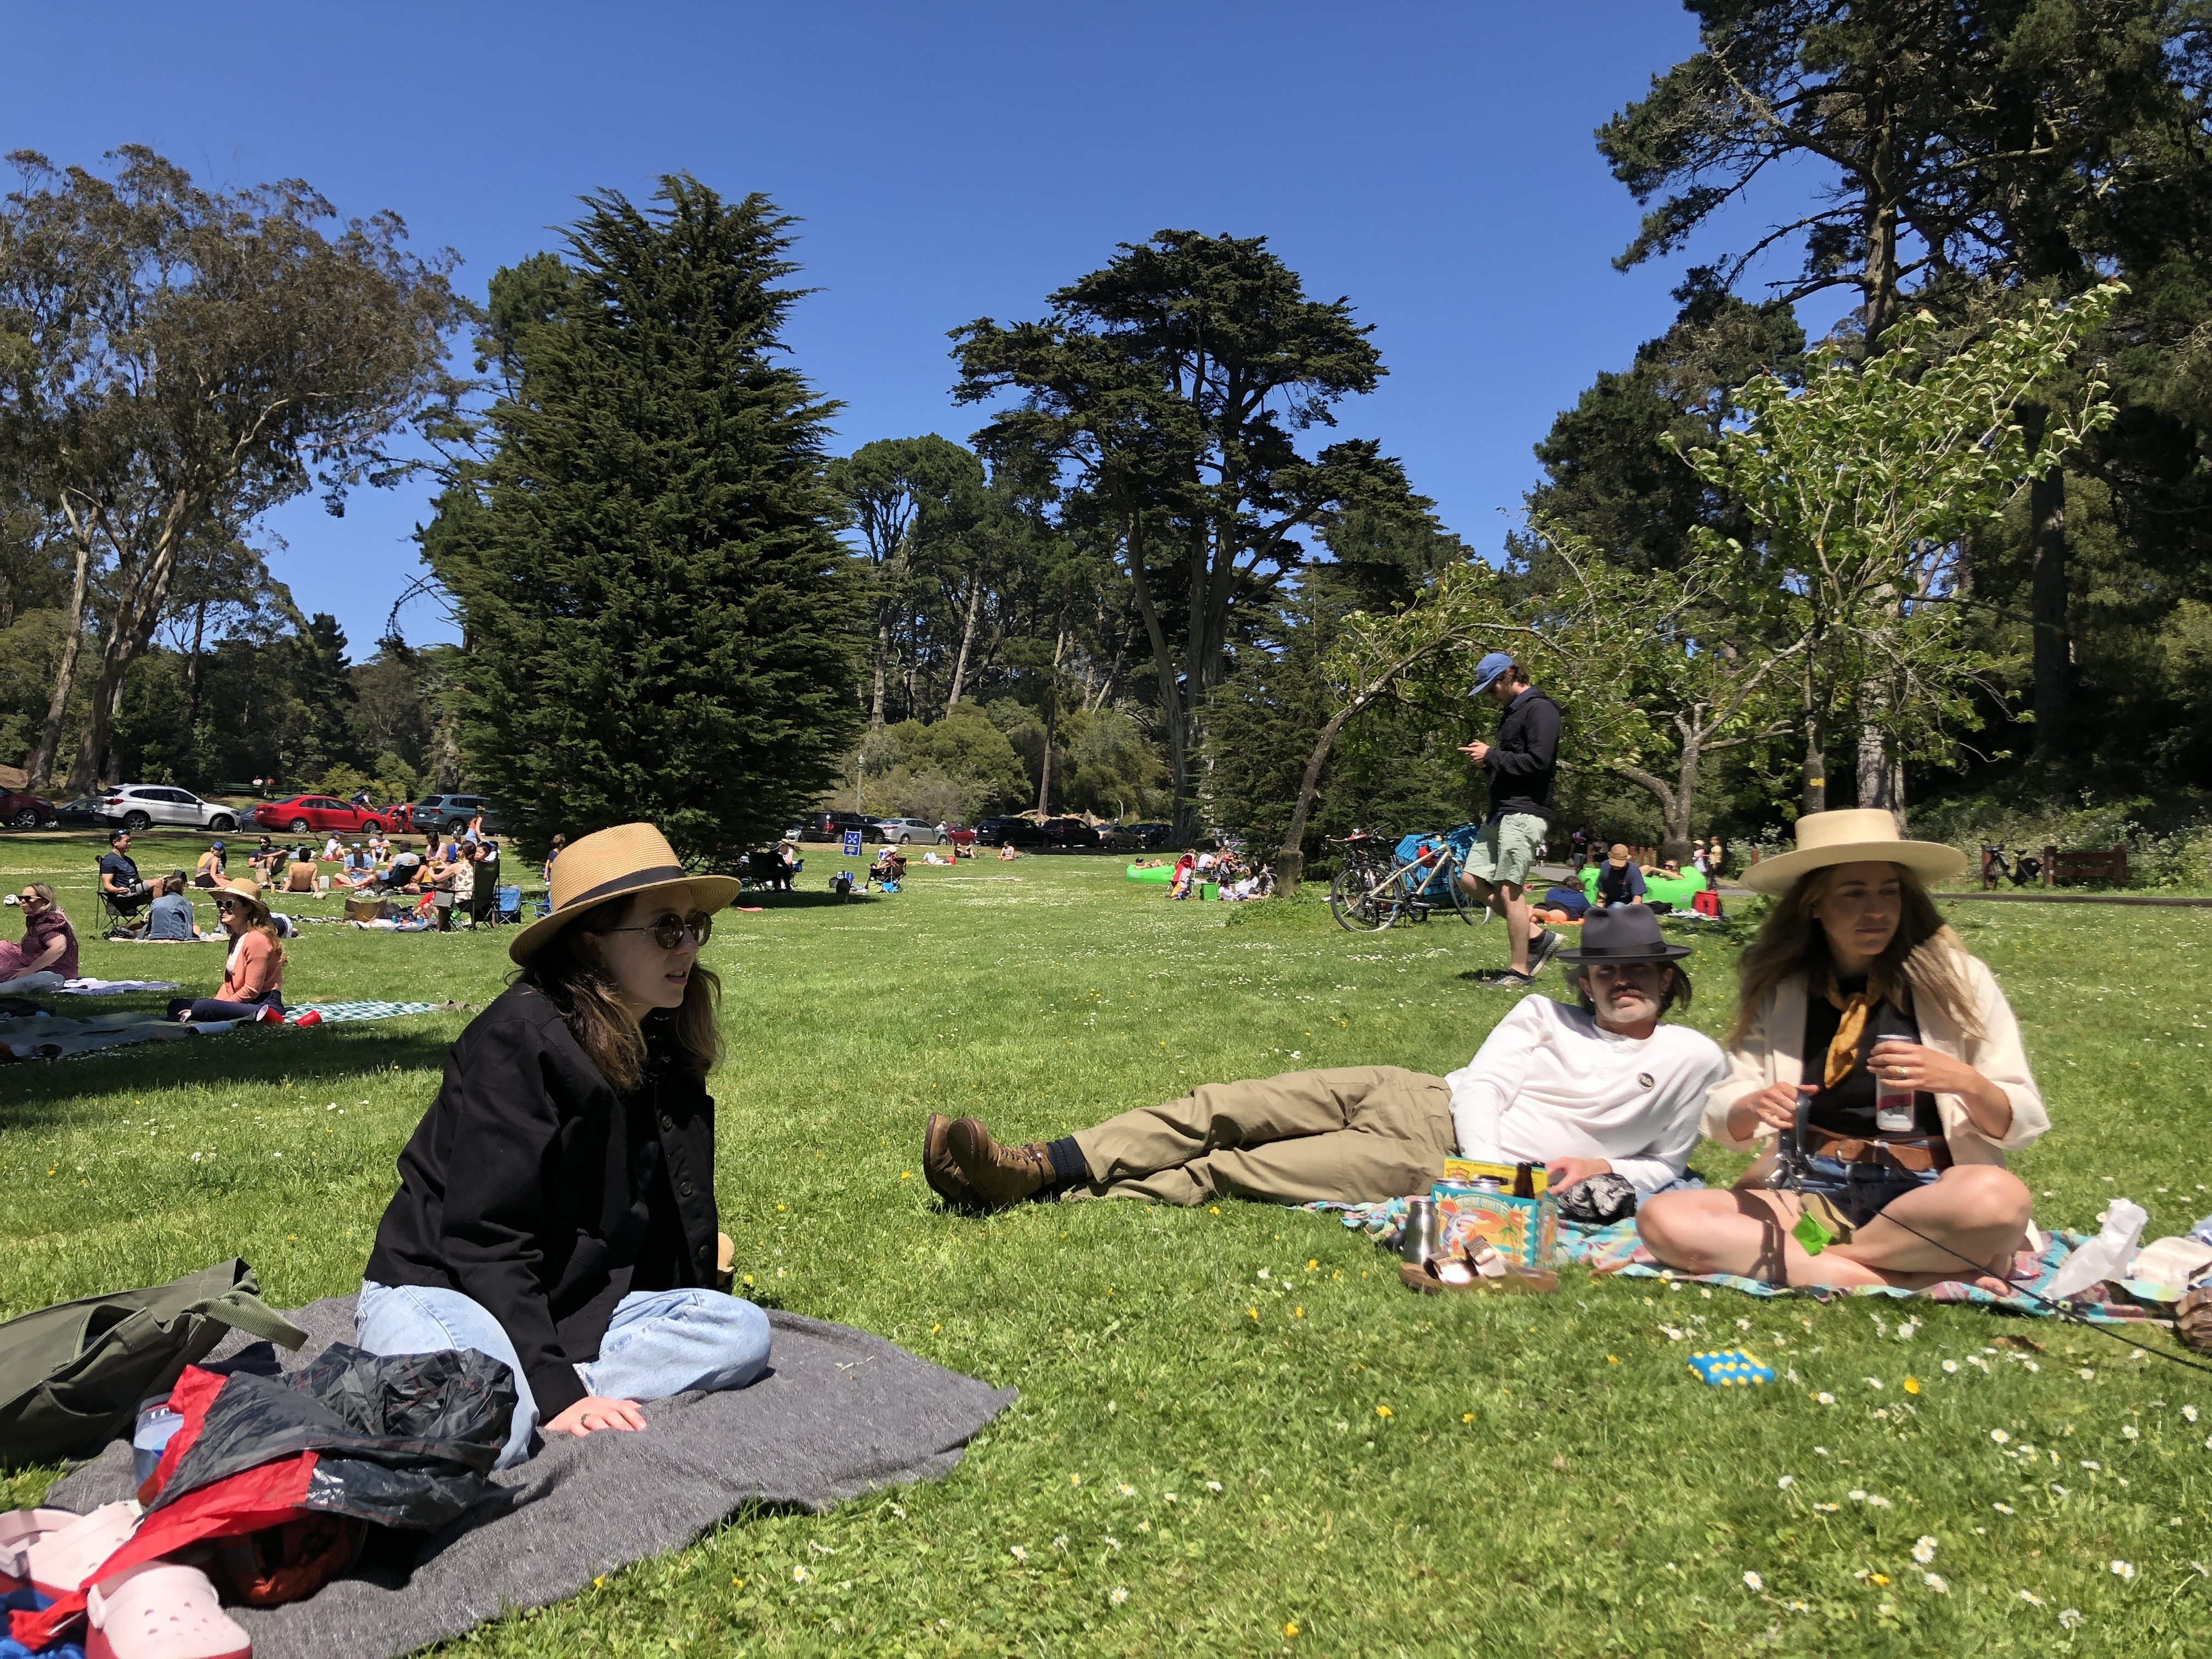
\includegraphics[width=0.8\textwidth]{images/introduction/ggp.jpg}
  \captionsetup{width=0.8\linewidth}
  \caption[Golden Gate Park]{Outdoor social gatherings in Golden Gate Park in San Francisco, United States, taken in May 2020 by the author.}
  \label{fig:golden_gate}
\end{figure}

\begin{multicols}{2}

\section{Background}
\subsection{"The pandemic"}
As known cases of SARS-CoV-2, colloquially referred to as COVID-19 or Coronavirus, started to increase in the spring of 2020, urban areas around the world came to a standstill. Normally traffic-clogged roads were empty, shops and restaurants closed, and the few people out walking dogs or picking up groceries protected themselves from infection by wearing masks, goggles, and gloves. From March through June 2020 in New York City, the urban chaos caused by COVID-19 was concentrated inside hospitals pushed to their limits to save patients from the new virus that proved to be fatal for 9.2\% of infected people and 32.1\% of hospitalized patients \cite{thompson_covid-19_2020}.

According to Merriam Webster, the words added to their lexicon in March and April 2020 included: COVID-19, community spread, social distancing, physical distancing, super-spreader, contactless, and more \cite{noauthor_coronavirus_nodate}. Social distancing, for example, is defined by Merriam Webster as "the practice of maintaining a greater than usual physical distance (such as six feet or more) from other people or of avoiding direct contact with people or objects in public places during the outbreak of a contagious disease in order to minimize exposure and reduce the transmission of infection" \cite{noauthor_social_nodate}. The addition of these words shows just how quickly the world of face-to-face interactions became a threat to human existence.  

Furthermore, public health directives not only discouraged in-person social interactions but in some cases enforced it with lockdown measures, travel restrictions, and curfews \cite{geng_impacts_2021}. The use of public spaces was prohibited, events were canceled, public transportation was to be taken sparingly, and school and work places transitioned to be fully remote. Citing the mental health consequences of limiting social interaction, the term “social distancing” was called into question by Thomas Abel and David McQueen in their March 2020 editorial for the International Journal of Public Health \cite{abel_covid-19_2020}. The authors called for a change in semantics, from social distance to spatial distance. Spatial distance refers to the public health advice of maintaining a two meter distance between people from different households, but the authors encouraged creative ways of nurturing social closeness to prevent the above-mentioned consequences of severing all social ties in the face of a long-term public health crisis.

For those without personal vehicles, the sudden shift to remote working and reduced public transportation service left only the amenities accessible by foot. Moreover, due to the unknown nature of the infectious disease, many people avoided leaving their homes altogether and there was an immediate increase in grocery delivery and restaurant takeout orders as a result \cite{wang_adoption_2021}. As more epidemiological information was known about COVID-19, people began seeking ways to see friends and family while maintaining the advised six-foot (two-meters) “social distance.” Those with backyards could host friends and family outdoors while maintaining the recommended distance, but this was generally limited to people living in less-urban areas. Residents of urban areas without private outdoor space could instead use public parks to be social, to exercise, and to experience the mental health benefits of being outdoors, as seen in Figure \ref{fig:yoyogi_park} from May 2020 in Tokyo's Yoyogi Park \cite{bereitschaft_how_2020}\cite{japan_yoyogi_2020}. 

\end{multicols}

 \begin{figure}[h!]
  \centering
  \includegraphics[width=0.8\textwidth]{images/introduction/yoyogi2.jpeg}
  \captionsetup{width=0.8\linewidth}
  \caption[Yoyogi Park]{Outdoor social gatherings in Yoyogi Park, May 2020 \cite{japan_yoyogi_2020}.}
  \label{fig:yoyogi_park}
\end{figure}

\begin{multicols}{2}

\subsection{Picnics of the past}
According to Levy (2014), documentation, literature and artist interpretations of gathering to eat a meal outdoors (a picnic) can be traced back to historical civilizations, including the Babylonians, Greeks and Romans. Ancient examples of picnics, though not called as such, consisted of a journey from shelter (home) to nature (fields) to eat a meal, typically with a noble or religious purpose \cite{levy_picnic_2014}. 

In more recent times, too, the idea of sharing a meal outdoors, away from home, spans a variety of cultures and geographic locations. Of the cities analyzed in this study--London, New York City, and Tokyo--each have their own histories relating to the experience of a picnic, and even to the parks included in this study. As early as 1654 CE, Oliver Cromwell, an important political figure in Britain, was documented dining on the grass of Hyde Park in London \cite{levy_picnic_2014}. Later, in twentieth century US, the proliferation of the picnic occurred alongside that of the automobile, as the freedom of the open road could bring one to a place to experience the freedom of eating outdoors \cite{levy_picnic_2014}. The celebration called Ohanami in Japan---a gathering underneath the blooming cherry blossom trees that involves the consumption of food and drinks---can be traced back to the Heian era (794-864 CE) \cite{moriuchi_sustainability_2019}. 

Eating a meal outdoors is not a novel concept, but the ease with which it is now possible is vastly different from the picnickers of the past. Instead of a home-cooked meal carefully prepared, packaged and transported to the site, restaurants offer take-out and grocery stores offer ready-made meals which significantly ease the experience. What remains the same, however, is the opportunity to gather with friends, share a meal, and enjoy the natural environment. 

\subsection{Neighborhoods}
A city neighborhood typically is not a definable attribute of the urban environment. In a US city, a neighborhood might be larger than a block, but smaller than a zip code. The neighborhood as an urban unit was introduced in the 1920s by Clarence Perry, Jane Jacobs called to bolster urban neighborhoods in the 1950s, and the movement gained momentum again in the last ten years with the "fifteen-minute city" concept proposed by Carlos Moreno \cite{jacobs_death_2020}\cite{moreno_introducing_2021}\cite{pozoukidou_15-minute_2021}. The idea then drew close attention in early 2020 in light of the global pandemic amid lockdowns and travel restrictions enacted to keep city residents local and prevent the spread of disease. Public transportation normally allows people to leave their neighborhoods on a daily basis to expand access to amenities. However, using the context of the recent pandemic, this research aims to discover whether city neighborhoods are sufficiently providing access to certain amenities without the use of public transportation. To do this, the neighborhoods closest to city parks will be analyzed to determine if they are well-positioned for local residents to make use of the park for outdoor social gatherings. 

An additional component to a social gathering experience, though not a requirement, is procuring food from home or on the way to the park. Areas around public transportation hubs typically attract retail and restaurants, but those areas became less populated during the pandemic as many companies issued work-from-home policies and restaurants closed to indoor dining \cite{hidalgo_amenity_2020}. Therefore, if public transportation is not considered when analyzing social gatherings in city parks, the neighborhoods can be assessed for the viability of a social gathering entirely within walking distance, from home to a food source to the park, and then back to home (see Figure \ref{fig:concept_diagram}).

\end{multicols}

 \begin{figure}[h!]
  \centering
  \includegraphics[width=0.9\textwidth]{images/introduction/concept_diagram.png}
  \captionsetup{width=0.9\linewidth}
  \caption[Concept diagram]{Concept diagram showing city residents traveling from home to a social gathering location while picking up food along the way.}
  \label{fig:concept_diagram}
\end{figure}\par

\begin{multicols}{2}

\section{Project description}
\subsection{City parks}
While much existing research on parks and their associated benefits is related to physical activity, this study will focus on the social potential of parks. Many other forms of public or semi-public spaces make up the fabric of a city (transit stations, shopping centers, town squares and plazas, etc.), but a park provides the additional benefits of being a natural environment with fresh air, open space, and cooler temperatures \cite{aram_urban_2020}. 

The parks included in this research (Hyde Park in London, Prospect Park in New York City, and Yoyogi Park in Tokyo) are city parks that do not require an admission fee. They are located within densely populated cities and are surrounded by both residential and commercial uses. They also have similar characteristics: open grass lawns, bodies of water, forested areas, and various other amenities like sports facilities, playgrounds and ancillary buildings that house restrooms, snacks and maintenance equipment. Due to the urban surroundings of the three parks, vehicular parking is limited. Furthermore, each of the chosen parks are notable destinations in their respective cities for locals and tourists alike. 

\end{multicols}

\begin{figure}[h!]
\centering
\includegraphics[width=0.70\textwidth]{images/introduction/prospect1.png}
\captionsetup{width=0.70\linewidth}
\caption[Prospect Park]{Outdoor social gatherings in Prospect Park, Brooklyn, New York City, United States, photographed in  May 2020 \cite{noauthor_ny_2020}.}
\label{fig:prospect_park}
\end{figure}\par\hspace{10pt}

\begin{figure}[h!]
\centering
\includegraphics[width=0.70\textwidth]{images/introduction/hyde2.jpeg}
\captionsetup{width=0.70\linewidth}
\caption[Hyde Park]{Outdoor social gatherings in Hyde Park, London, England, photographed in May 2022 \cite{sanderson_green_2023}.}
\label{fig:hyde_park}
\end{figure}

\begin{multicols}{2}

\subsection{Hyde Park in London, England}
Hyde Park began as private hunting grounds that were partially opened to the general public as early as 1637 CE and is now one of eight Royal Parks in London \cite{noauthor_history_nodate}. In 1665 CE, shortly after its public debut, the grounds of Hyde Park were used as camping grounds for city residents to escape the plague \cite{noauthor_history_nodate}. This is exemplary of the relationship between public health and parks, even in the seventeenth century when few public parks existed. More recently, as cities have developed across the country, Shaori et al. (2021) found that the median space available in all parks in England and Wales is about 4.9 square meters per person. During a pandemic this leaves many areas of the country at risk for overcrowdedness \cite{shoari_accessibility_2020}.

\subsection{Prospect Park in New York City, USA}
Prospect Park was designed in the 1860s after the US Civil War, with the goals of replicating the appeal which Central Park brought to Manhattan and to improve the health and well-being of the people living in the New York City borough of Brooklyn \cite{tate_great_2013}. Currently, New York City is estimated to average around 3.64 square meters of park space per capita, with a relationship between greater park area and higher incomes by zip code \cite{noauthor_park_nodate}. 

\subsection{Yoyogi Park in Tokyo, Japan}
Tokyo's Yoyogi Park was formerly a military facility and opened to the public in 1963 \cite{havens_parkscapes_2011}. As in Europe and North America, the addition of parks into urban areas of Japan came from a call to solve public health issues and to provide infrastructure and open space during other disasters, both human and natural. The division of the Japanese government in charge of public parks was within the Hygiene Bureau as of the Grand Council order of 1873; and, according to Havens (2017), the division's main purpose was to protect the health of people. As green space increased in the early twentieth century, more uses were found for parks such as firebreaks and evacuation sites after earthquakes. According to the Tokyo Bureau of Construction, as of April 2020, there are 5.73 square meters per capita of park space in Tokyo, surprisingly high given the population density of the metropolis \cite{noauthor_parks_nodate}.

\subsection{Comparing physical attributes}
Table \ref{table:city_parks} provides an initial comparison of the physical attributes of the parks and the cities within which they are located. The population density is based on the city as a whole (see Appendix B for data resources), and the coordinate reference system (CRS) is used for the various analyses conducted in geographic information system (GIS) software in later chapters. As expected, each park has different strengths and weaknesses: Hyde Park has the highest quantity of entry points but London is the least dense city of the three; Prospect Park has the largest area and perimeter, but less entry points than Hyde Park; and Yoyogi Park opened most recently of the three parks but despite Tokyo being the densest city studied, with only five entry points there is an entry per 653 meters of perimeter length, likely a weakness when finding the park's accessibility.

\subsection{Parks for health and social interaction}
A common characteristic influencing the development of each of the above-mentioned parks is public health. As will be further discussed in Chapter \ref{chapter_03}, the relationship between pandemics, the health of city residents, and city parks has repeated itself throughout history. For this reason, many existing studies about the benefits of city parks exist, and the below research aims to add to this body of research through the lens of social interaction within the context the most recent public health crisis.

\end{multicols}

\begin{table}[H]
\small
\begin{tabular}{llccccccr}
\toprule
{} &      {} &  Pop. dens. &          CRS &  Year &  Area &  Perimeter &  Entry &  Perimeter \\
Park name &      City &  (per $ km^{2}) $ &          (EPSG) &  open &  $ (km^{2}) $ &  $ (m) $ &  points &  to entry \\
\midrule
Hyde Park &    London &             5701 &  27700 &          1637 &       1.40 &          5639.1 &            24 &                 235 \\
Prospect Park &  New York &            11314 &   2263 &          1866 &       1.80 &          6705.0 &            17 &                 394 \\
Yoyogi Park &     Tokyo &            15462 &  32654 &          1963 &       0.56 &          3266.6 &             5 &                 653 \\
\bottomrule
\end{tabular}
\caption[City parks]{Comparing the physical attributes of Hyde Park, Prospect Park, and Yoyogi Park.}
\label{table:city_parks}
\end{table}

\begin{figure}[H]
  \centering
  \includegraphics[width=1.0\textwidth]{images/introduction/process.png}
  \captionsetup{width=1.0\linewidth}
  \caption[Chapter diagram]{Diagram of chapter outline and analysis methodology.}
  \label{fig:process}
\end{figure}

\begin{multicols}{2}

\section{Chapter outline}
Chapter 2 reviews existing research on walkability in urban neighborhoods, thermal comfort and public space, city parks and the recent COVID-19 pandemic, and relevant uses of image classification and network analysis methodologies.

Chapter 3 provides a brief historical overview of city parks and their relationship to various crises of the times. Chronologically, this begins with England and the cholera pandemics of the nineteenth century. In the United States urban parks were developed to offset further urban development in many cities and after the Great San Francisco Earthquake of 1906, used to house those whose homes were destroyed. In Japan, park infrastructure was a way to “modernize” the country when its borders opened to the outside world \cite{havens_parkscapes_2011}. 

Chapter 4 defines the conditions for outdoor social gatherings. Then, satellite imagery is used in combination with various GIS tools to locate and quantify potential areas for the social gatherings in the three city parks studied throughout this research.

Chapter 5 uses the results from Chapter 4 along with government census and OpenStreetMap data to determine how many people live around the above-mentioned parks and, moreover, how many have access to social gathering spaces and food amenities. The software used in this chapter includes QGIS as well as the UNA Toolbox for Rhino. 

Finally, Chapter 6 presents the results of the social gatherings capacities compared to population of the surrounding neighborhoods. One might expect that a park with many social gathering opportunities will also be well-connected to the surrounding neighborhood. However, since the quantity of social gathering opportunities was likely not a factor in park design, the reason for the well-connectedness can be understood by the physical features of the park and the neighborhood. Of the three parks analyzed in this study---Hyde Park, Prospect Park, Yoyogi Park---the park with the most ideal access is uncovered, providing a measurement to work towards when considering how other city parks could change to better prepare the urban environment for the next pandemic.

\end{multicols}

\textit{"How much a park is used depends, in part, upon the park's own design. But even this partial influence of the park's design upon the park's use depends, in turn, on who is around to use the park, and when, and this in turn depends on the uses of the city outside the park itself."}\\
---Jane Jacobs, \textit{The Death and Life of Great American Cites} (1961)
\cleardoublepage

%the cleardoublepage command ensures that the next text page is on the right-hand side (odd page) and produces a blank page if necessary to achieve that, as all chapters should begin on the right hand side

\chapter{Literature review}
\noindent This research is inspired by the movement to strengthen urban neighborhoods that began in the previous century, but the context for this particular study stems from the recent global health crisis. Already, many scholars have addressed the urban challenges resulting from the COVID-19 pandemic. However, the specific goal of quantifying social gatherings in city parks has yet to be accomplished in existing studies. The literature review below provides initial insight into the concepts and methodologies used in the research that follows.\\

\begin{figure}[h]
  \centering
  \includegraphics[width=1.0\textwidth]{images/literature/theory.png}
  \captionsetup{width=1.0\linewidth}
  \caption[Literature review]{Literature review themes and applicable references.}
  \label{fig:literature}
\end{figure}

\begin{multicols}{2}

\section{Walkability in urban neighborhoods}
From a perspective of safety and the context of urban exodus in the mid-twentieth century US, Jacobs (1961) writes that city neighborhoods should be planned to "foster lively and interesting streets," be a continuous network throughout a subsection of a city, and to function as districts in and of themselves. According to Jacobs, parks and public spaces should "knit together the [urban] fabric's complexity and multiple use" instead of isolating neighborhoods \cite{jacobs_death_2020}. Similarly, Gehl (2011) advocates for the \textit{lively} street, where people can see and be seen, a condition which increases the possibility for social interactions in the urban environment. Outdoor activities in the urban environment are divided into three categories by Gehl: necessary, optional, and social. Social activities "depend on the presence of others in public spaces" and the physical conditions of the environment directly influence pedestrian quantity, length of time spent outdoors, and the activities which occur \cite{gehl_life_2011}. 

More recently, but before the pandemic, a resurgence in the neighborhood movement was spearheaded by Carlos Moreno in 2016 with the "15-minute City" concept. The idea being that high-quality urban life is inversely proportional to time spent using transportation. Through density, diversity, digitalization and proximity of urban services, Moreno et al. (2021) propose interconnected neighborhoods where residents can meet their needs within a fifteen-minute pedestrian or cycling trip from home \cite{moreno_introducing_2021}. Separately, Ross et. al (2021) finds recreational walking to be one factor that contributes to individual "flourishing" in a neighborhood \cite{ross_walking_2021}. 

Pozoukidou and Chatziyiannaki (2021) write about the renewed importance of walkable cities in the face of the COVID-19 pandemic, and how cites around the world were actively making policy changes in the face of the public health crisis. The authors divide city policies into three pillars: inclusion, health and safety, and evaluate the overall proximity of amenities on a neighborhood scale \cite{pozoukidou_15-minute_2021}. Loftata et al. (2022) also cover the topic of neighborhood walkability and the social implications of COVID-19 pandemic restrictions. Their research employed surveys to understand the changing patterns of residents in cities around the world, finding that access to basic amenities by 15-20 minute walking distance and social cohesion became critical during the pandemic \cite{lotfata_changing_2022}. 

\section{Thermal comfort and public space}
The work of Matzarakis and Mayer (1997) and Matzarakis et al. (1999) relating physiological equivalent temperature (PET), thermal perception, and grade of physiological stress is significant when considering comfort in outdoor public spaces \cite{matzarakis_urban_1997}\cite{matzarakis_applications_1999}. Further, Höppe (1999) relates PET to air temperatures in the winter sun and shade and summer sun and shade, providing a point of reference for understanding the relationship between the two conditions. Using these concepts, many researchers have since conducted behavioral studies to understand how thermal comfort is experienced in public spaces. Nikolopolou et al. (2001) determined thermal neutrality of urban spaces in Cambridge, England to range from 7.5 degrees Celsius in the winter to 27 degrees Celsius in the summer, and further found that users eating and socializing preferred sunlight and warm conditions to shade \cite{nikolopoulou_thermal_2001}. 

Thorsson et al. (2007) studied temperature in relation to urban space in Japan using structured interviews, observations of behavior, and micrometeorological measurements to compare a public square and public park in the same town. The park was found to be cooler than the square, both in actual temperature measurement and in terms of calculated physiological equivalent temperature (PET) value. In addition, a relationship was found between the perceived thermal conditions and the amount of time the respondents spent in the public space \cite{thorsson_thermal_2007}.

Vidal et al. (2022) used the environmental psychology data collection technique called Behavioral Mapping (BM) to identify patterns of behavior in Public Urban Green Spaces (PUGS). Among other findings, the study shows that natural areas are less likely to be used than areas that are manicured or contain urban furniture like benches, and that sunny but not excessively hot days are the most desirable for using the public spaces. Their conclusion was therefore that future green space designs should use vegetation to shape the space, including clearings for picnics, and to integrate both sunny and shaded areas so that users can make a choice depending on the weather and their needs \cite{vidal_patterns_2022}. 

\section{City parks and COVID-19}
Geng et al. (2021) conducted a global study of pandemic impacts on park visitation, finding that in most countries park visitation increased after February 2020. Using stepwise regression analysis to compare daily confirmed cases of COVID-19, Google Mobility data on park visitation before and after the pandemic, and government policies relating to the public health crisis, it was found that stay-at-home orders and restrictions on public transportation were the most significant factors negatively correlated with changes to park visitation. Interestingly, the least significant factor was the daily increase in the number of known cases of COVID-19, showing that an increase in cases did not increase or decrease park visitation \cite{geng_impacts_2021}. 

Furthermore, the Geng et al. study includes the three the countries featured in this research: United States, England (UK), and Japan. For Japan---alongside Italy, Spain, South Korea, and Sweden---it was found that there was not a significant change to park visitation when COVID-19 began \cite{geng_impacts_2021}. The authors suggest that this was a result of the government response and restrictions, but the paper does not compare access to parks in any of the studied countries. It is possible that park visitation could not change during the pandemic in cities that do not have an abundance of accessible parks. 

Park visitation during the pandemic was also studied by Rice and Pan (2021) through Google's open-source mobility trend data, finding that season and age of population had an affect on park usage during the pandemic that mobility data did not account for. The authors call for park design that creates ample social distancing opportunities in order to improve the physical and social well-being of a population during a pandemic \cite{rice_understanding_2021}.

Shaori et al. (2020) study park space allocation per person for England and Wales when considering COVID-19 pandemic-related social distancing recommendations. The authors use 500 and 1000 meter buffers around postal codes to quantify per capita park space \cite{shoari_accessibility_2020}. The results found postal codes with four square meters of green space per person to be inadequate for meeting social distancing needs, likely leading to overcrowded parks. The study is important for analyzing park access on a national level, but using postal codes for population data can lead to aggregation error in the results. The research that follows uses smaller administrative boundaries and focuses on three specific parks to understand accessibility at a finer level of detail. 

Pipitone and Jović (2021) study equitable access to green space during pandemic conditions. Through online surveys they found that the COVID-19 pandemic expanded the socio-spatial inequities already present in New York City \cite{pipitone_urban_2021}. Also in the US, Farboodi et al. (2021), calculated the cost of social risk during the COVID-19 pandemic through cell phone tracking data and mobility reports. The study found that recreation activity in the US had recovered from the initial pandemic lockdown effects by July 1, 2020 \cite{farboodi_internal_2021}. Farboodi et al. conclude that individuals lowered their social activity in the first months of the pandemic to reduce the risk of infection, but since herd immunity is one solution to overcoming an infectious disease, people must weigh the risk of socializing on an individual level. 

\section{Analysis methodologies}
The research that follows will make use of several different spatial analysis methodologies. The first applied technique is object-based image classification, which uses aerial imagery for land-cover mapping. Ma et al. (2017) perform a meta-analysis on the research methodologies used in 173 scientific papers. According to their findings, the methodology of supervised object-based image classification is quickly advancing in the field, and an area-based method is found to be more accurate than the point-based method \cite{ma_review_2017}. 

Thapa and Murayama (2009) analyze image classification approaches for urban land use in the city of Tsukuba, Japan. The land use classes used by Thapa and Maruyama include urban forest, lawn/grass, paddy field, dry farmland/exposed field, facility/industry, residence/parking/road, and water. The four classification approaches used were unsupervised, supervised, fuzzy supervised, and GIS post-processing, which extracted the matching features from the first three approaches and was found to be the most accurate method \cite{thapa_urban_2009}. In the same city, Lwin and Murayama (2011) model urban green space through the combined methodology of remote sensing, GIS and spatial web technology. The resulting "eco-friendly walk score calculator" allows residents to determine either the shortest route (for shopping activities) or the greenest walking route (for recreational activities) \cite{lwin_modelling_2011}. 

Population studies are used to analyze the spatial distribution, amenity distribution, and population characteristics within a research area. The spatial distribution of age is analyzed by Andersson et al. (2018), finding the relationship between localized access to amenities and how the age of neighborhood reflects the priorities of people in that age group \cite{andersson_urban_2018}. As mentioned above, Shaori et al. (2020) used population data and park allocation to determine access to parks during the pandemic. In this study, population catchment will be analyzed to estimate the population of residents within walking distance to a park compared to the social gathering capacity within the park. 

The distribution of urban amenities is a widely-studied topic using a variety of methodologies. Hidalgo et al. (2020) use spatial analysis techniques to find amenities that are over and under supplied in neighborhoods throughout the US. Clustering algorithms identify neighborhoods by amenity density, and then the model compares predicted versus actual number of amenities. The authors find in cities like Tokyo and London, amenities cluster around transit stations due to the number of daily riders, but "exogenous destinations" that also attract amenities include dense residential or employment areas, busy intersections, and public facilities and open spaces \cite{hidalgo_amenity_2020}.

Caballero and Tsukamoto (2006) discuss the concept of "dividual space," which is the idea of private physical spaces within commercial facilities in Tokyo. The authors propose that public space is not equivalent to "collective" space, which is why amenities like karaoke and internet cafes that provide space to rent by the hour for individuals or small groups are popular across Japan \cite{caballero_tokyo_2006}. This supports the pandemic-driven concept of social gathering spaces that are available for use by individuals and small groups in the research that follows. 

Beeco and Brown (2013) review methodologies for finding the capacity of parks and protected areas (PPA) to allow for use without a resource deteriorating due to the quantity of visitors. The authors describe the different needs of trail users who seek out established trail routes compared to "urban socials" who need urban parks for large social gatherings \cite{beeco_integrating_2013}. In other words, from the perspective of resource conservation, the capacity of natural spaces should be determined to prevent overuse and deterioration of the environment. 

Spatial access to public open space (POS) during the recent pandemic is analyzed by Habibullah et al. (2022), by quantifying park access within a one-kilometer walking distance in the city of Jeddah, Saudi Arabia. The public open spaces are categorized by average area including local/pocket, neighborhood, district/city, regional, and national/metropolitan parks. Analyzed by district, the results show the percentage of the population that had access to public open space within one kilometer \cite{habibullah_one-kilometer_2022}.  

Marako et al. (2009) write about the complications of determining access to parks in New York City. Their findings reveal parks to not be equitably distributed geographically, meaning the ability for residents to be physically active is not geographically equal across the city. Further, they emphasize the importance of using entry points to measure access because a neighborhood can border a park without there being a way to physically enter the space \cite{maroko_complexities_2009}. In other words, the entry points of parks might reveal a lack of access despite proximity to certain neighborhoods.

\section{Originality}
A substantial amount of research has been conducted on parks, neighborhood amenities, COVID-19, and some combination of those three topics. However, there does not seem to be existing research quantifying outdoor social gatherings in city parks. Moreover, there does not appear to be research assessing the accessibility of social gatherings in parks while considering food amenities and the surrounding population. This research will make use of methodologies similar to those used in the above existing research, especially the combined use of image classification and network analysis methodology implemented by Lwin and Murayama (2011). This study aims to contribute to the growing literature on access to city parks, with access being important both in times of “normalcy” and during a public health crisis. 

\end{multicols}


\cleardoublepage


\chapter{City parks and times of crisis}\label{chapter_03}
"To improve and expand urban disaster facilities and plans, new urban parkland should be infrastructural and multi-functional; they should be used as a daily part of urban life while maintaining the mechanisms needed to support local community and to respond to natural or unexpected disasters."---Noboru Masuda (2014)

This chapter will cover a brief history of city parks, especially as they have related to times of urban crisis and disaster. From the spread of cholera in the 1820s, to the most recent global public health crisis that began in 2020, city parks are an important part of the urban infrastructure. This section will provide historical context for the evolution of city parks and help set the stage for how parks might need to change in response to the COVID-19 pandemic.\\
 
\begin{multicols}{2}

\section{City parks} 
Originally, green spaces in many European cities and throughout Japan were not public spaces, instead reserved for the wealthy and the elite \cite{havens_parkscapes_2011}\cite{jones_equity_2009}. The establishment of city parks began around the same time urban life was changing dramatically due to the Industrial Revolution. Industrialization, overcrowdedness, and infectious diseases made cities unhealthy and unpleasant, and city parks were seen as a solution to these problems \cite{malchow_public_1985}\cite{jones_lungs_2018}. 

Across Europe, many green spaces were owned by royal families until the nineteenth century. One of the earliest examples of a green space created for the public was in Paris in 1605 CE, when the king had the Place de Vosges constructed as a place for respite from the overcrowded city \cite{jones_lungs_2018}. In London, several royal parks transitioned from royal hunting grounds to public space, including Hyde Park in 1637 \cite{jones_lungs_2018}. Later, Birkenhead Park in England opened in April 1847---now known to be the first publicly funded urban park \cite{tate_great_2013}. In 1943 the County of London Plan aimed to provide more green space to improve the health of people \cite{hill_forshaw_2005}, showing the connection between public health and parks continued into the twentieth century.

In the US in the 1850s, New York City was densely crowded and infected with cholera, tuberculosis, and other diseases, according to Cranz (1989). Public health officials argued for the establishment of Central Park "because they observed that clean air helped reduce the spread of disease" \cite{cranz_politics_1989}. Early twentieth century then saw a rise in neighborhood parks and playgrounds to provide a place deemed as safe for children to play. Perhaps because parks were considered public space, civic uses were commonplace, such as army recruitment in the 1920s, and during the Great Depression parks were used recreation as a means of social control by diversion from issues such as unemployment \cite{cranz_politics_1989}.

City parks in Japan were influenced by those in Europe and the US in the nineteenth century around the time of the Meiji Restoration. According to Havens (2011), Edo delegates were sent from Japan to Europe and the United States in 1860 to "investigate the secrets of capitalist modernity," one of the findings being parks in the US, England and France. Before this visit, much green space already existed in Japan in the form of temples and gardens, but like many other countries, it typically belonged to the high-ranking and wealthy \cite{havens_parkscapes_2011}. The advocates of the early city parks in Japan saw the many benefits of the open spaces: recreation, disaster relief, political control, hygiene, and curbing infectious diseases \cite{havens_parkscapes_2011}. 

In each of the cities studied, city parks have been associated with times of national crisis since their inception as public space. Shortly after Hyde Park opened to the public in the seventeenth century, the grounds were used for city residents to escape the plague \cite{noauthor_history_nodate}. In the mid-nineteenth century, authorities in both England and US sought parks as the solution to "population growth, hygiene, mortality and communicative disease" with Victoria Park in London opening in 1845 to stop spreading epidemics \cite{jones_lungs_2018}. Also in London, to prepare for air raids during World War II, trench shelters were built in parks and open spaces \cite{ainsworth_geophysical_2018}. 

An example of the relationship between parks and disasters in the US is the use of Golden Gate Park in the aftermath of the 1906 San Francisco earthquake as a place for the displaced to set up refugee camps \cite{cranz_politics_1989}. During the Great Depression, recreation programs were created as relief for the unemployed in San Francisco, and in New York, Works Progress Administration (WPA) workers were assigned to park construction and maintenance projects during this same time \cite{cranz_politics_1989}. During World War II, parks hosted first aid classes, provided space for barracks and other military activities, and operated as community gardens for vegetables and flowers \cite{cranz_politics_1989}. 

\end{multicols}

\begin{figure}[h]
  \centering
  \vspace{8pt}
  \includegraphics[width=1.0\textwidth]{images/crisis/timeline.png}
  \captionsetup{width=1.0\linewidth}
  \caption[Timeline diagram]{Comparative timeline showing the history of city parks and disaster events for England, the United States and Japan.}
  \label{fig:timeline}
\end{figure}\par

\begin{multicols}{2}

In Tokyo, parks are closely tied to the disasters that have impacted the city. After the 1923 earthquake and fire, the government of Tokyo created a design plan for the city which used public parks and open spaces as firebreaks and refuge areas after a seismic event \cite{masuda_disaster_2014}. The reconstruction plan of November 1923 encouraged the establishment of parks for public health, rest and relaxation during ordinary times, and in the case of an emergency, for fire prevention, evacuation and relief \cite{havens_parkscapes_2011}. During World War II, parks not only served as firebreaks, but also housed soldiers in training, were used for farming and firewood, as refuge for the homeless, and more \cite{havens_parkscapes_2011}. Masuda (2014) explains that the urban park as a disaster refuge "should include a warehouse, earthquake-proof water tank, radio broadcasting facilities, helicopter pad, and fire fighting facilities" \cite{masuda_disaster_2014}. More recently, the benefits of parks include air quality improvement, serving as windbreaks and helping to reduce global warming by absorbing carbon dioxide \cite{havens_parkscapes_2011}.

Figure \ref{fig:timeline} shows a comparative timeline of the history of city parks and disaster events for England, the United States and Japan. There are clear influences between the three countries in this study regarding park implementation and design. Frederick Law Olmsted visited Birkenhead Park in England in 1850 CE before designing Central Park in New York in 1866 CE. Around the same time, delegates from Japan visited cities in Europe and the United States, bringing back to Japan the inspiration to build city parks \cite{havens_parkscapes_2011}.

From the perspective of governmental agencies, incentives to create and maintain city parks across time, geography and culture, are for the perceived notions of public health and social control, and for encouragement of leisure and recreation \cite{jones_lungs_2018}\cite{cranz_politics_1989}\cite{havens_parkscapes_2011}. The initial movement to create public parks in cities came as a response to the overcrowdedness which led to outbreaks of cholera and other diseases. Then, as wars erupted, natural disasters occurred, and eventually the occurrence of the recent pandemic, parks have been utilized to protect city residents.

\section{Crisis management}
Wisner and Adams (2002) write about emergency response strategies for the protection of the people and the environment in emergencies and disaster situations. The authors differentiate three phases as planning, prevention, preparedness and mitigation; emergency response; recovery, rehabilitation and reconstruction to promote sustainable development and, further, the authors express the importance of preparing for future disasters during "normal" times \cite{wisner_environmental_2002}.

The top diagram in Figure \ref{fig:crisis_management} shows the disaster management cycle from Wisner and Adams (2002), and then further adapts the diagram to express the disaster response cycle in relation to city parks. The middle diagram shows an impact as an earthquake, fire, war, or pandemic. As discussed previously, there are many examples across time and geography where city parks were used in response to a disaster. This includes evacuation and refugee centers after earthquakes and for farming or army training during a war. After each disaster and subsequent new uses, it is typical for legislation to be passed to improve existing parks or add new parks to better serve a city in the face of the next disaster. 

Amid the recent COVID-19 pandemic, city parks were used across the world for people to exercise, enjoy nature, socialize with friends despite the ongoing spread of disease \cite{bereitschaft_how_2020}. The bottom image in Figure \ref{fig:crisis_management} represents the response and mitigation efforts with the pandemic as the disaster impact event. The initial response to the spread of COVID-19 included lockdowns, cancelled events, and stay-at-home orders which restricted residents from leaving their homes except for "essential" activities \cite{storr_essential_2021}. As more information about the disease was understood, the public health response transitioned from the emergency response to recommendations for how to live with the spread of disease. Some of the resulting recommendations included masking requirements in public spaces, resumed service of public transportation, and the encouragement of low-risk social gatherings in outdoor spaces. 

Using the past disaster impacts and resulting changes in planning policy to better prepare city parks for future disasters, the research that follows will try to determine what might be changed to prepare three city parks for the next pandemic.

\end{multicols}

\newpage
\null
\vfill
\begin{figure}[H]
  \centering
  \captionsetup{width=0.9\textwidth}
  \includegraphics[width=0.9\textwidth]{images/crisis/crisis_management.png}\par\hspace{3pt}
  \caption[Crisis management diagram]{Top diagram: disaster management cycle, adapted from Wisner and Adams (2002) \cite{wisner_environmental_2002}; middle diagram: disaster management cycle relating to city park evolution; bottom diagram: disaster management cycle with COVID-19 as the disaster impact.}
  \label{fig:crisis_management}
\end{figure}


\cleardoublepage


\chapter{Image classification of social gathering locations}\label{chapter_04}
\noindent Social distancing recommendations enacted during the COVID-19 pandemic meant many public and private urban spaces unusable for social activities. During this time, city parks were one of the few places that could provide space for people to meet with a relatively low risk of contracting COVID-19. In order to prepare city parks for similar use in future pandemics, this chapter will identify appropriate locations for social gatherings using image classification tools. Then, the results will be used to quantify the existing capacity of social gatherings in Hyde Park in London, Prospect Park in New York City, and Yoyogi Park in Tokyo.\\

\begin{figure}[h]
  \centering
  \includegraphics[width=0.9\textwidth]{images/gatherings/domino_park.jpeg}
  \captionsetup{width=0.9\linewidth}
  \caption[Domino Park, NYC]{At Domino Park in New York City, painted circles encouraged social distancing in May 2020 \cite{cogley_white_2020}.}
  \label{fig:domino_park}
\end{figure}

\begin{multicols}{2}

\section{Low-risk social gatherings}
\subsection{Domino Park case study}
In March and April of 2020 when COVID-19 was rapidly spreading in New York City, infection rates and insufficient hospital capacities led to an alarmingly high number of fatalities, instilling a fear that prevented many residents from leaving their homes \cite{thompson_covid-19_2020}. Then, as new infections slowed and people began to emerge from their homes, the park director of Domino Park in New York City decided to reconcile the opposing needs of social distancing and social interaction \cite{strauss_how_2020}. On May 15, 2020, circles were drawn with chalk paint on the grass lawn of Domino Park, eight-feet (2.4 meters) in diameter and six feet apart (1.8 meters) (see Figure \ref{fig:domino_park}) \cite{cogley_white_2020}. 

The dimensions of the Domino Park social gathering circles allow one to four households (one to four individuals per circle) to socialize while maintaining two-meters of physical distance, as depicted in Figure \ref{fig:circle_dims}. Moreover, and importantly during a pandemic, the physically drawn circle provides a sense of enclosure or personal space that reminds park visitors of public health recommendations to maintain low-risk social gatherings. While the size and spacing of the Domino Park circles could be the subject of their own research, this study will make use of the dimensions described above to test the existing capacity of social gatherings in other city parks. 

Furthermore, although socialization typically occurs between at least two people, the analysis that follows will include gathering circles occupied by just one person or a single household. Even without a pandemic, there are individuals who use a park alone and feel comfortable sitting near other visitors even without interacting \cite{peters_social_2010}. Therefore, it can be assumed that during the heightened stress of a pandemic, some people would make use of the gathering circles to enjoy the park in the comfort of their own outdoor space, while surrounding by others doing the same.
\end{multicols}

%\begin{multicols}{2}

%\end{multicols}

\begin{figure}[h]
  \centering
  \includegraphics[width=0.9\textwidth]{images/gatherings/circle_dims.png}
  \captionsetup{width=0.9\linewidth}
  \caption[Outdoor gathering circles]{Using the dimensions from Domino Park, this diagram illustrates how social distancing circles can be used by different groups.}
  \label{fig:circle_dims}
\end{figure}

\begin{multicols}{2}

\subsection{Park programming}
The Domino Park social gathering circles are an important case study because they are a proactive yet minimal change to the programming of a park. Many prominent city parks were built early in the last century and funding even for maintenance can be scarce, meaning major design changes do not occur often \cite{havens_parkscapes_2011}. While this research will not propose changes to park programming or design, future studies could use the social gathering quantities discovered below compared to the population studies in Chapter \ref{chapter_05} to advocate for changes that would increase the social gathering capacity of the parks in this study. 

Parks are designed, by necessity, with entry points along the perimeter and with the main internal programming of the park relatively inaccessible except by foot. This allows visitors to feel like they are in nature and far away from the city, but it also means that the distance to the conveniences of the city can be felt \cite{jones_lungs_2018}. Cranz (1989) describes how even for park visitors in the early twentieth century, the expectation was that a day in the park would include amenities such as refreshments, restrooms, lighting, and benches \cite{cranz_politics_1989}. 

The parks in this study are large in area, ranging from 0.56 to 1.8 square kilometers, which means the entrances along the perimeter are not an insignificant walking distance to interior areas suitable for social gatherings. Once visitors enter the park, leaving the park to get food---at a restaurant, food shop, or home---would typically signal the end of the park visit due to the travel distance and time it would take to accomplish those tasks and then return. Therefore, it is assumed that many park visitors who have planned a social gathering in advance would acquire food before entering the park. Typically, large parks contain on-site refreshments, but since maximum capacity of the park is of interest as well as the visitors' variety of options, the next chapter will include sourcing food for social gatherings from outside the park as well as within (see Chapter \ref{chapter_05}).

\section{Research conditions}
\subsection{Where to have an outdoor gathering}
While the most essential criteria for an outdoor social gathering is to be outdoors, there are many factors that contribute to the human comfort and therefore probability of such an event. First, the space must be public and open for people to use at their leisure during the day. This study has not included parks that demand an entrance fee, because even if minimal, a fee reduces the number and equity of potential visitors. Furthermore, while many public plazas could fit most of the conditions below, parks are more often used and more suitable for outdoor gatherings \cite{thorsson_thermal_2007}. Even though picnic tables and benches are part of the landscape of a park, this study will focus on areas where visitors can sit directly on the ground. The additional conditions below will define a suitable outdoor social gathering space for the purpose of this study.

\subsection{Conditions for an outdoor gathering}\label{conditions}
\textit{Grass or non-pavement ground cover}\\
The surface of the ground is an important feature for determining gathering locations. Hard surfaces such as pavement are uncomfortable for long periods of time, and therefore roads and paved paths will not be included for potential gathering areas. Ideally the ground is grass or a similarly soft surface, and not an excessively moisture-absorbing or heat-absorbing material (both sand and turf are less ideal than natural grass for this reason). 

\textit{Larger than 100 square meters in area}\\
Many sources have suggestions for the ideal size of public space. The goal in defining a minimum area for social activities is to eliminate areas of a park that might be identified as suitable for a social gathering by image classification software, but would not in reality be used by park visitors due to the remoteness or scale. The New York Planning Department uses a minimum public plaza size of 2000 square feet, or about 185 square meters \cite{noauthor_privately_nodate}. UNhabitat recommends an area of 0.03 to 0.04 hectares (300 to 400 square meters) for the smallest category of public space called "local/pocket open public spaces" \cite{noauthor_public_nodate}. Zagora and Šamić (2021) use a minimum dimension of 25 meters to define small and extra-small scale public spaces presented in their study \cite{zagora_urban_2021}. Similarly, Gehl (2011) describes 20 to 25 meters to be a socially interesting and relevant distance because it becomes possible to perceive the feelings of surrounding people \cite{gehl_life_2011}. For the purpose of this study any area smaller than 100 square meters is not included in the analysis. 

\textit{No gatherings on sports fields or courts}\\
In the context of a pandemic, playing sports outdoors is generally a low-risk transmission activity similar to an outdoor social gathering. Athletes should therefore still be able to use these program areas for their intended purpose, even if they contain grass lawns which could be used for social gatherings instead. Sports fields will not be analyzed for their social gathering capacity in this study.

\textit{No gatherings within 50 meters of main roads}\\
The parks chosen for this study are large parks that provide visitors with a sense of nature and escape from the city. Because they are all located in dense cities, they are all surrounded by major roads. Gehl (2011) coined the term 'pedestrian city,' for which a distance of 50-100 meters is recommended to transfer from a vehicular landscape (city limits or edge of a residential area) to the local neighborhood \cite{gehl_life_2011}. For this reason, a distance of 50 meters from major roads is utilized to create a visual and auditory barrier between car traffic and the park experience. 

\textit{No gatherings within 10 meters of buildings}\\
Similar to above, most visitors to a park want to feel as if they are in nature, and being near a building would disrupt this feeling. A distance of 10 meters from the exterior of any ancillary park building is recommended based on observations at Yoyogi Park.

\textit{Weather determines sun/shade preferences}\\
While many attributes of Hyde Park, Prospect Park and Yoyogi Park are similar, the most divisive difference is their geographic locations, which create vastly different climatic conditions. Section \ref{thermal_comfort} will determine how thermal comfort informs the ideal locations for outdoor social gatherings in each of these parks.

\vspace{5pt}
\begin{minipage}{0.45\textwidth}
    \centering
    \includegraphics[width=\linewidth]{images/gatherings/OBIA_legend.png}\par\captionof{figure}[Image classification legend]{Image classification legend for the land-cover categories used in this study.}
    \label{fig:obia_legend}
\end{minipage}
\vspace{5pt}

\section{Methodology}
\subsection{Image classification}
Object-based image classification is a technique that uses aerial remote sensing data for land-cover classification \cite{ma_review_2017}. In this study, Google Earth aerial imagery and QGIS tools are used together to locate areas that meet the previously described conditions for social gatherings in the chosen parks \cite{noauthor_google_nodate}. Specifically, the Orfeo ToolBox (OTB) in QGIS is a remote sensing image processing tool that uses segmentation to convert groupings of raster pixels into vector objects that represent different land features \cite{neteler_compiling_2015}. 

While complex techniques for achieving highly accurate image classification results are described by Ma et al. (2017), this research uses sample points for five land-cover categories (see Figure \ref{fig:obia_legend}) to generate predicted values for the segmented vector objects \cite{ma_review_2017}. The land-cover categories include: (1) Building, (2) Dense planting (forest), (3) Grass lawn, (4) Paved surface (road), and (5) Water feature. Once the predicted values are generated, the resulting vector file is manually compared to the original aerial imagery and adjusted where the results are significantly different from the actual attributes of the park. Figure \ref{fig:obia_parks} shows the final adjusted classification results for Hyde Park, Prospect Park, and Yoyogi Park. 

\begin{minipage}{0.45\textwidth}
    \centering
    \includegraphics[width=\linewidth]{images/gatherings/hyde_OBIA.png}\par\hspace{5pt} 
    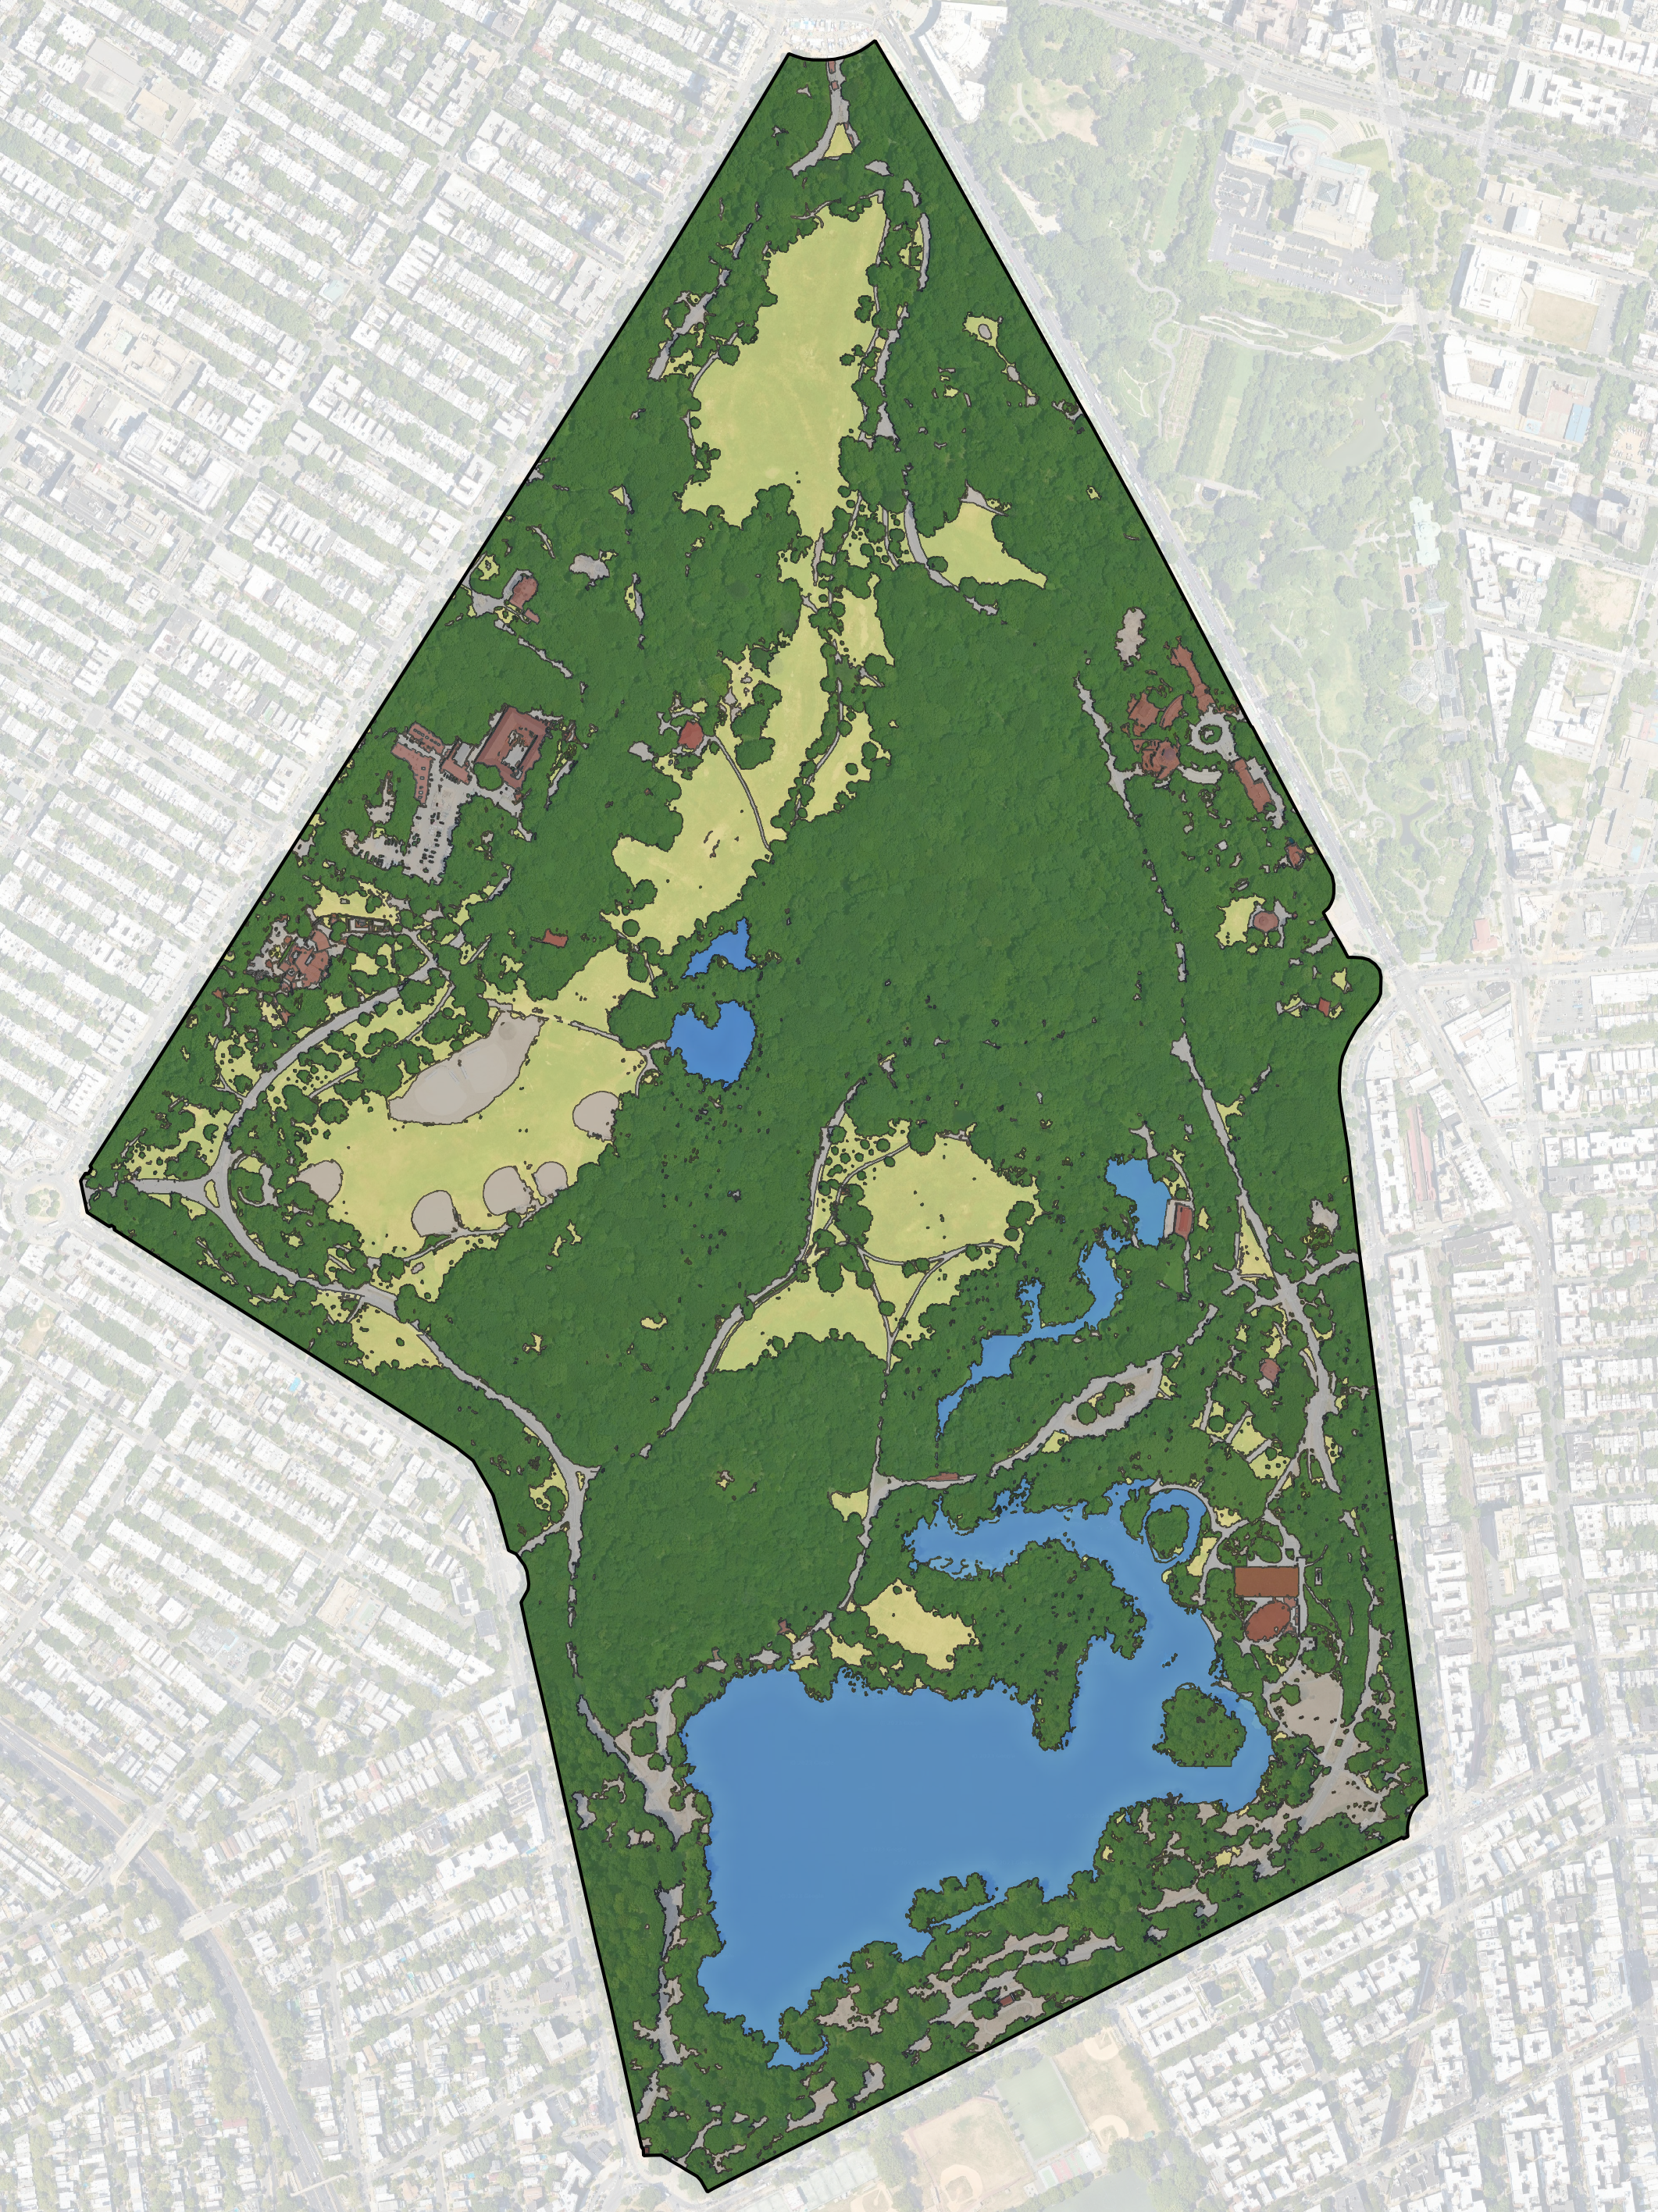
\includegraphics[width=\linewidth]{images/gatherings/prospect_OBIA.png}\par\hspace{5pt} 
    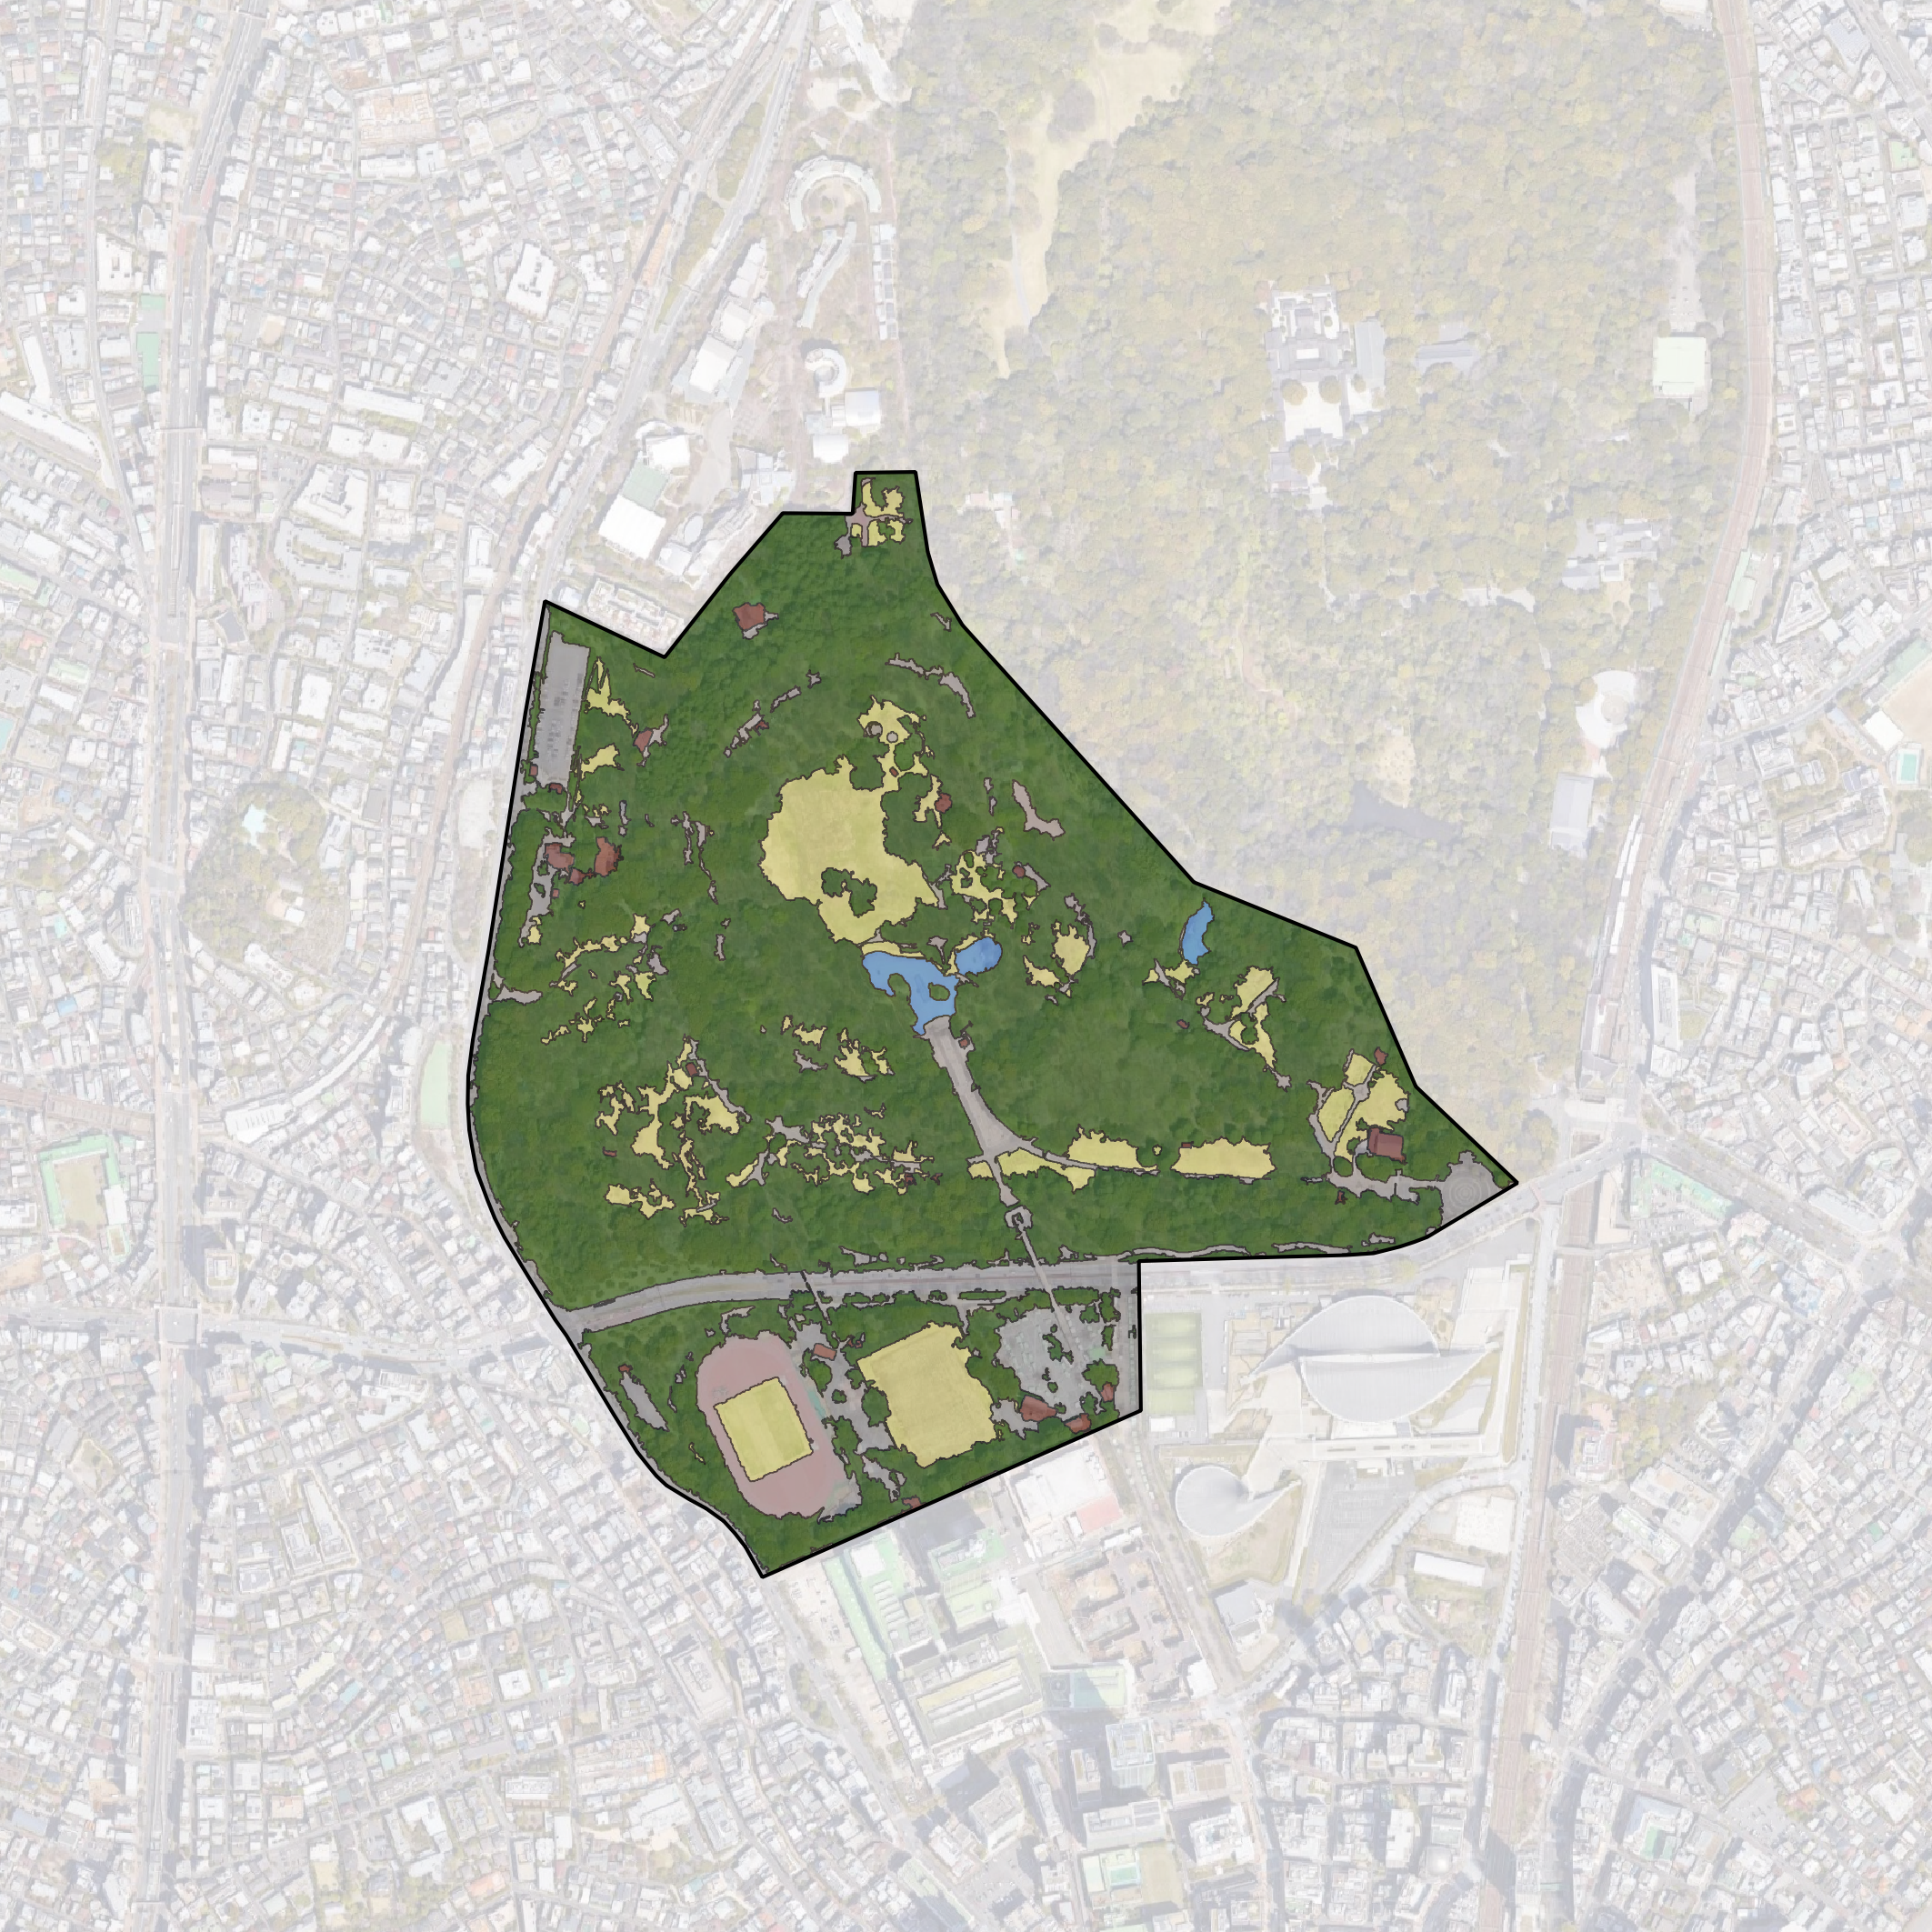
\includegraphics[width=\linewidth]{images/gatherings/yoyogi_OBIA.png}\par\hspace{5pt} 
    \includegraphics[width=\linewidth]{images/gatherings/scale_legend.png}\par\captionof{figure}[Image classification]{Top to bottom: Hyde Park, Prospect Park, and Yoyogi Park. Object-based image classification by land-cover category.}
    \label{fig:obia_parks}
\end{minipage}

\end{multicols}

\begin{figure}[h]
  \centering
  \includegraphics[width=0.7\textwidth]{images/gatherings/pie_charts.png}
  \captionsetup{width=0.7\linewidth}
  \caption[Classification pie charts]{Pie charts representing the percentage of park area for each land-cover category from the adjusted image classification models.}
  \label{fig:pie_charts}
\end{figure}\par
\vspace{5pt}

\begin{table}[h]
    \centering
    \small
    \begin{tabular}{lcrrrr}
    \toprule
    Park Name &  Class &  Predicted &  Adjusted & Percent & Percent\\
     &  ID &  Area $ (m^{2}) $ &  Area $ (m^{2}) $ & Change & of Park\\
    \midrule
    Hyde Park &         1 &           44275 &          18749 &     -57.65\% &                       1.35\% \\
     &         2 &          683667 &         659413 &      -3.55\% &                      47.48\% \\
     &         3 &          378250 &         398761 &       5.42\% &                      28.71\% \\
     &         4 &          152996 &         192620 &       25.9\% &                      13.87\% \\
     &         5 &          129711 &         119356 &      -7.98\% &                       8.59\% \\
    \midrule
    Prospect Park &         1 &           82665 &          23021 &     -72.15\% &                       1.28\% \\
     &         2 &         1157466 &        1172324 &       1.28\% &                      64.98\% \\
     &         3 &          264518 &         256300 &      -3.11\% &                      14.21\% \\
     &         4 &          105981 &         165239 &      55.91\% &                       9.16\% \\
     &         5 &          193539 &         187285 &      -3.23\% &                      10.38\% \\
    \midrule
    Yoyogi Park &         1 &           34684 &           5659 &     -83.68\% &                       1.01\% \\
     &         2 &          379617 &         397461 &        4.7\% &                       70.9\% \\
     &         3 &           99354 &          67473 &     -32.09\% &                      12.04\% \\
     &         4 &           42377 &          84667 &      99.79\% &                       15.1\% \\
     &         5 &            4536 &           5308 &      17.02\% &                       0.95\% \\
    \bottomrule
    \end{tabular}
    \caption[Predicted and adjusted image classification]{Predicted versus adjusted areas of the image classification analysis.}
    \label{table:OBIA}
\end{table}

\begin{multicols}{2}

\subsection{Classification results}
Although the attributes such as area and geographic location vary, each park contains grass lawns, forested areas, water features, sports facilities, ancillary buildings, roads and pedestrian paths. Figure \ref{fig:pie_charts} shows the percentage of coverage for the above-mentioned land-cover categories in each park, giving an initial point of comparison for how much space might be available for social gatherings. Each of the parks contain only one-percent of land dedicated to buildings, showing that the three parks likely have similar proportions of ancillary facilities dedicated to restrooms, concessions, and maintenance equipment. Hyde Park contains the highest proportion of grass lawn (29\%) and largest area (almost 400,000 square meters), followed by Prospect Park with roughly 256,000 square meters of grass lawn or 14\% of the whole park. Yoyogi Park has less than 70,000 square meters of grass lawn or 12\% of the park area; however, Yoyogi Park has the highest proportion of forest (dense planting) with 71\%, which increases the number of potential social gathering spaces due to the climate in Tokyo and the culture preferences for less sun (see Section \ref{thermal_comfort}). 

Shaori et al. (2020) uses the two-meter social distancing requirements to create a metric of four square meters per person in calculating the distribution of green space across England and Wales. While this would mean that a park the size of Hyde Park (1.4 square kilometers) would potentially reach a capacity of 350,000 visitors, this is unrealistic because 52\% of the park is dedicated to water features, roads, buildings, and dense planting areas as determined by the image analysis above. By identifying plausible social gathering areas, this study aims to find a more accurate predictor of the capacity of city parks. 

\subsection{Accuracy verification}
The accuracy of the image classification can be seen in Figure \ref{fig:obia_diff} using the legend in Figure \ref{fig:accuracy_legend}. To understand which categories were the most and least likely to be correctly identified, the percent change is calculated in Table \ref{table:OBIA} of the computer-predicted to the manually-adjusted areas. For Hyde and Prospect parks, the two categories that present the least change between predicted and adjusted models are Class (2) Dense planting and Class (3) Grass lawn. For all three parks, the two most incorrectly identified categories are (1) Buildings and (4) Paved surfaces. Because Class (2) and (3) are more important to this study, it is significant to note that these two classifications are generally predicted accurately.  

Finally, an overall accuracy value is determined in Table \ref{table:global_OBIA} by taking the percentage of the area of correctly identified vector objects compared to the total area of each park. Prospect Park is the most accurate model at 95\% and Yoyogi Park is the least accurate at around 83\%. This is likely due to the aerial imagery used, as the most recent Google Earth imagery for Yoyogi Park is from a winter month. In the image, the trees do not have leaves and therefore the image classification tool can not easily differentiate the trees from the ground surface. On the other hand, Prospect Park's imagery is from a summer month, so the contrast between the dark green of the trees and light green of the grass lawns is easily distinguished by both the computer and the human eye.

\begin{minipage}{0.45\textwidth}
    \centering
    \includegraphics[width=\linewidth]{images/gatherings/accuracy_legend.png}\par\captionof{figure}[Image classification accuracy legend]{Legend for the accuracy models of image classification analysis.}
    \label{fig:accuracy_legend}
\end{minipage}

\begin{minipage}{0.45\textwidth}
    \centering
    \includegraphics[width=\linewidth]{images/gatherings/hyde_OBIA_diff.png}\par\hspace{5pt} 
    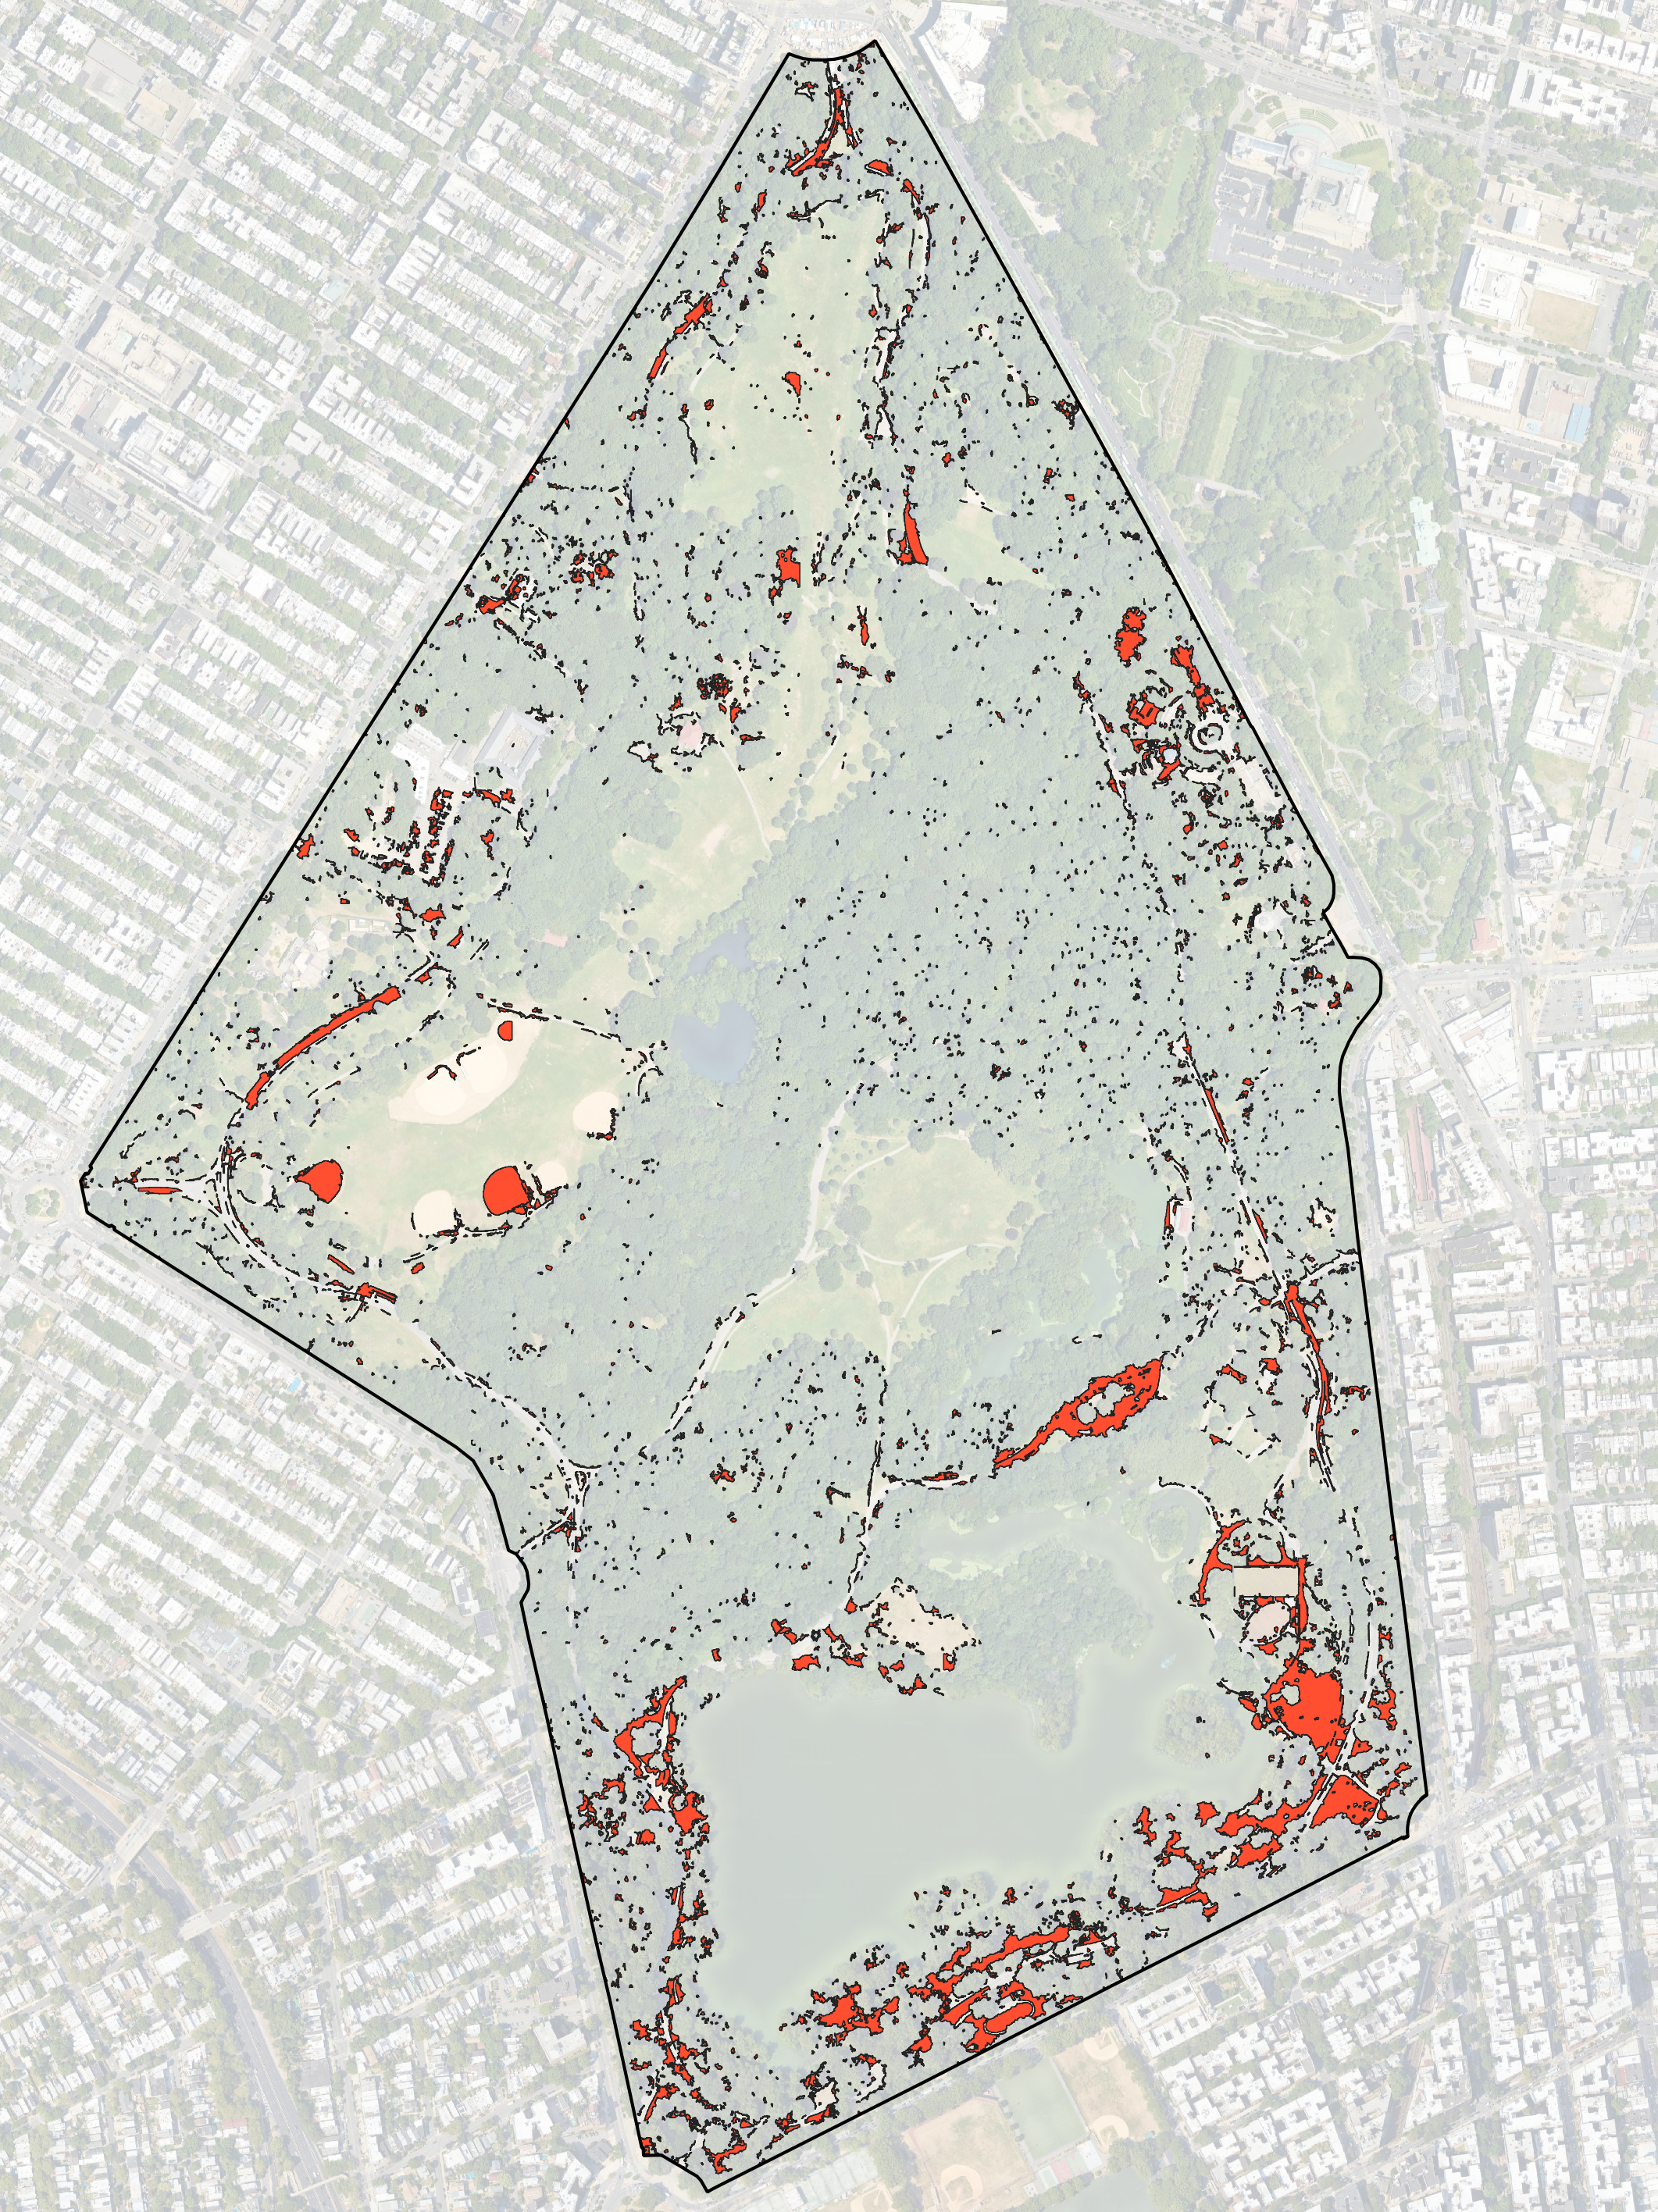
\includegraphics[width=\linewidth]{images/gatherings/prospect_OBIA_diff.png}\par\hspace{5pt} 
    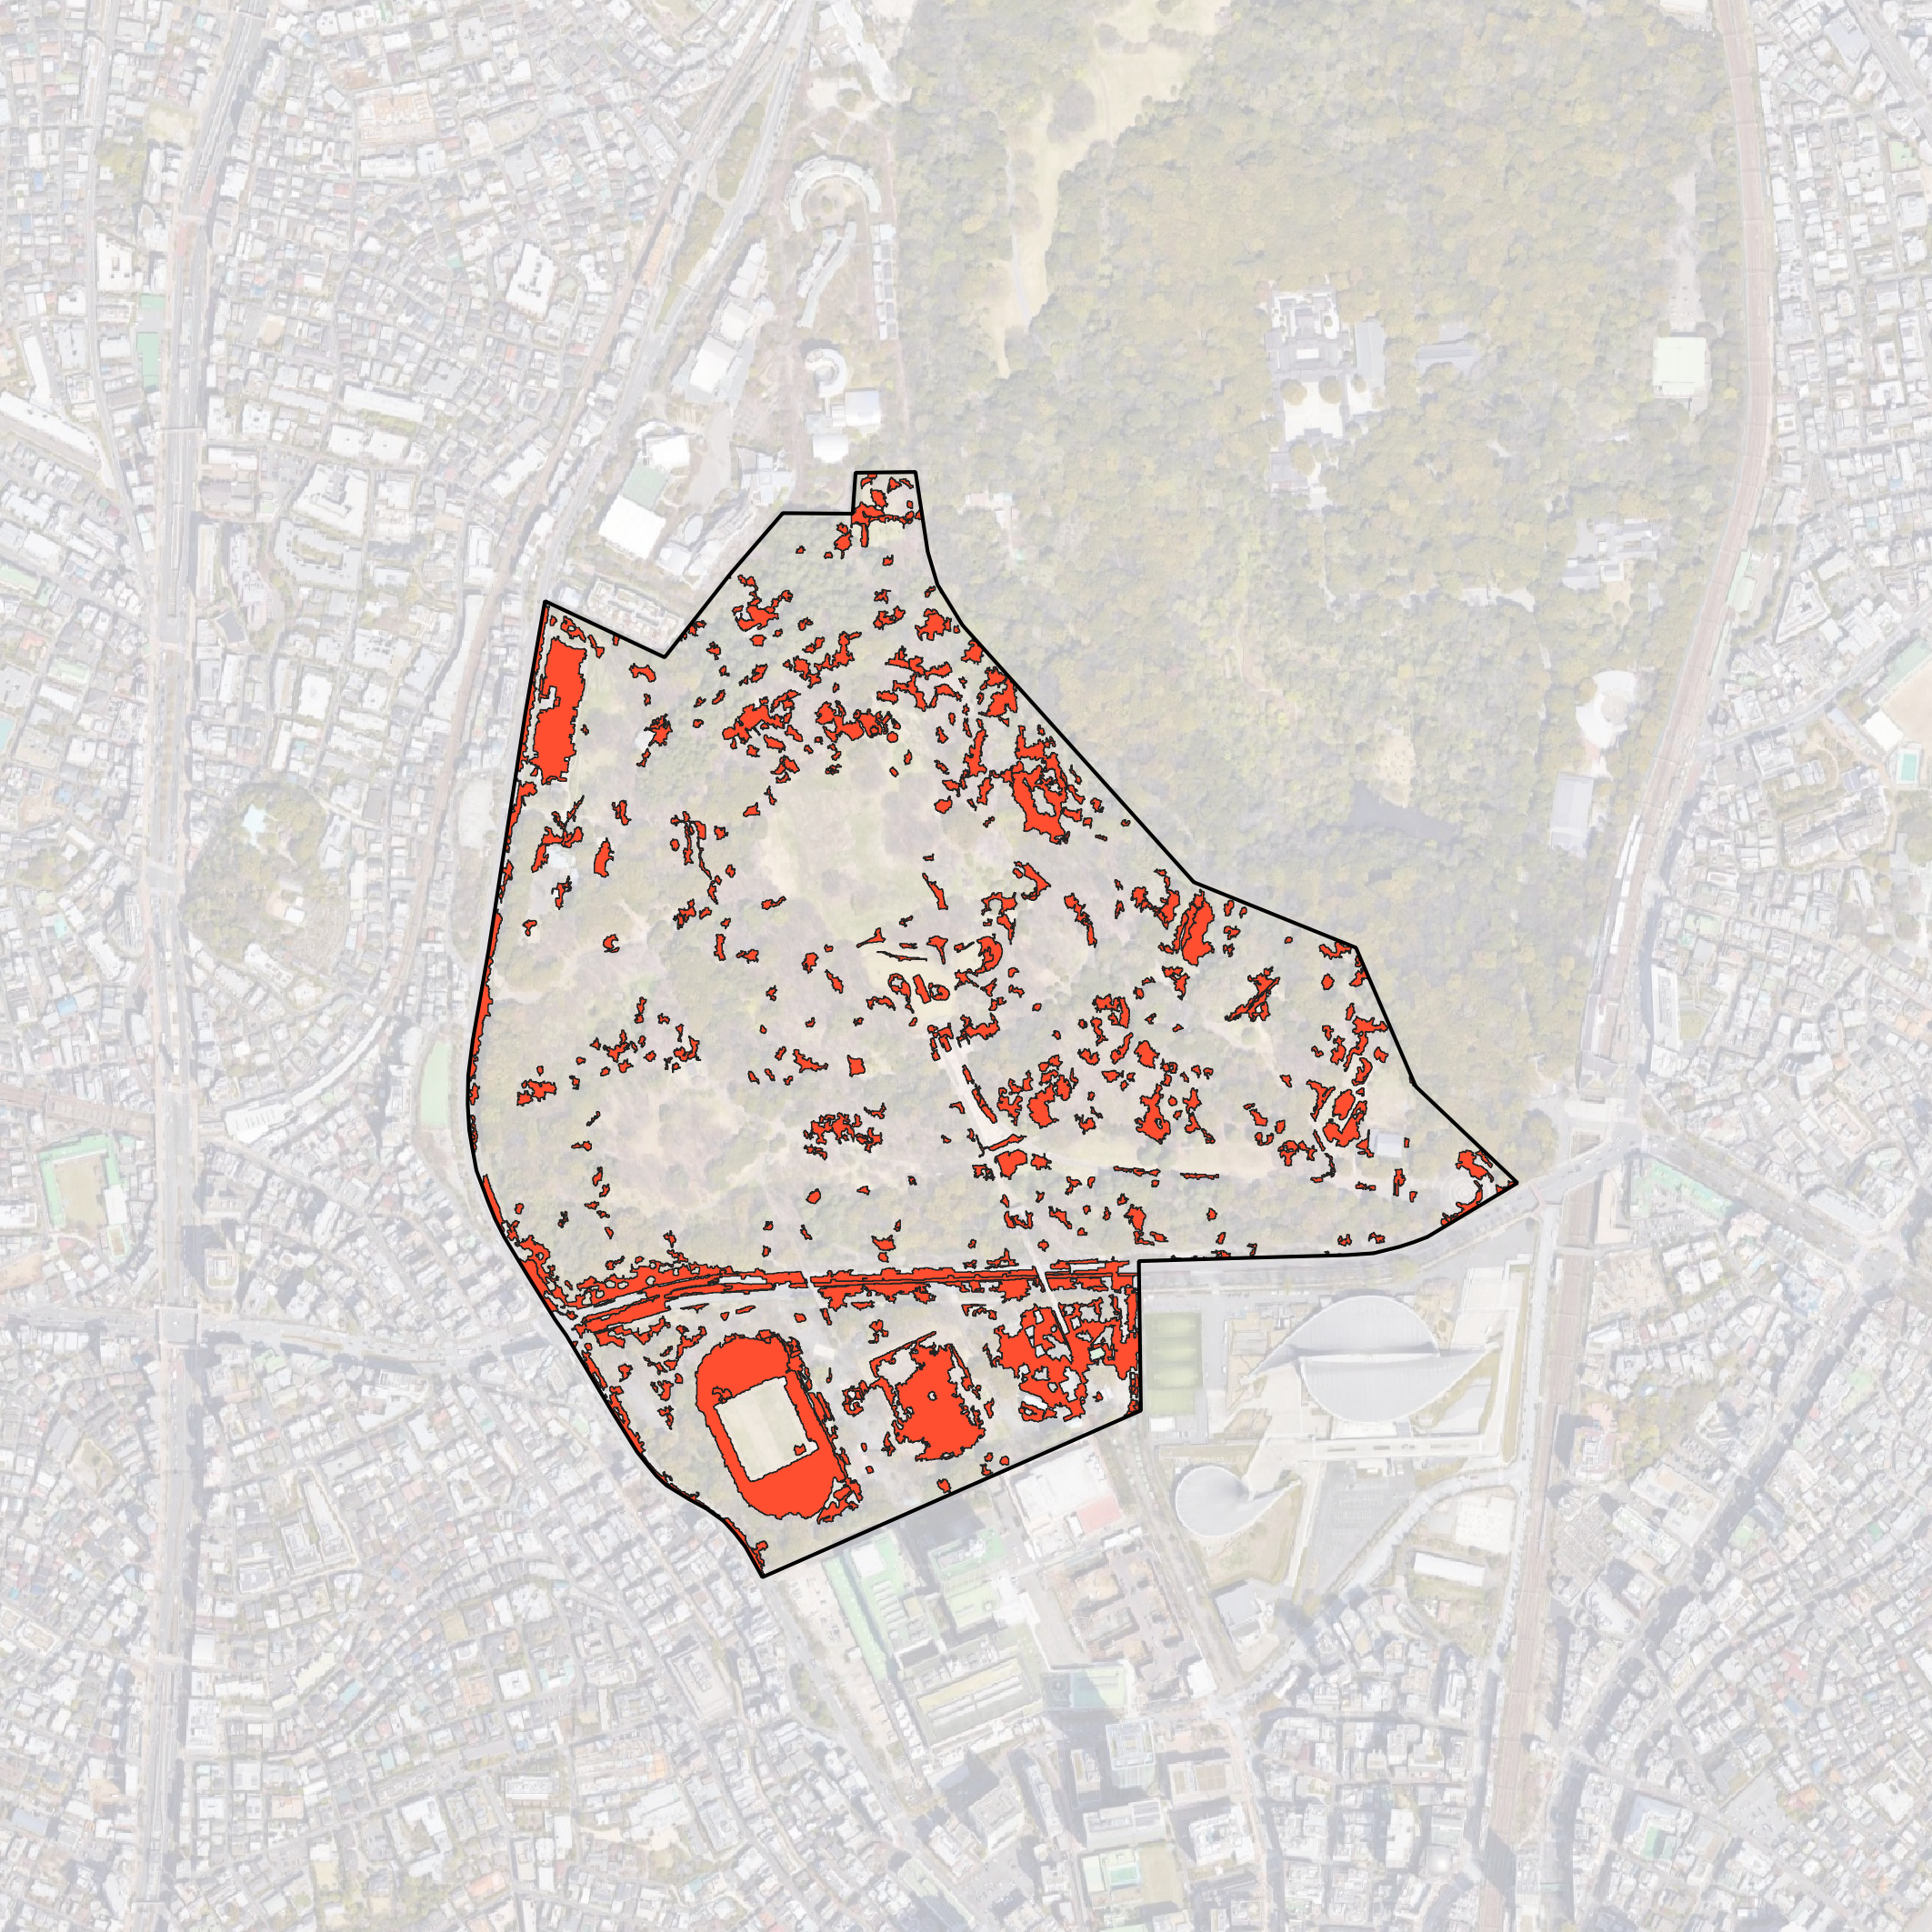
\includegraphics[width=\linewidth]{images/gatherings/yoyogi_OBIA_diff.png}\par\hspace{5pt} 
    \includegraphics[width=\linewidth]{images/gatherings/scale_legend.png}\par\captionof{figure}[Image classification accuracy]{Top to bottom: Hyde Park, Prospect Park, and Yoyogi Park. Discrepancies between predicted and adjusted image classification.}
    \label{fig:obia_diff}
\end{minipage}

\end{multicols}

\begin{table}[h]
      \centering
      \small
    \begin{tabular}{lr}
    \toprule
    Park Name &  Overall Accuracy \\
\midrule
Prospect Park &     95.07\% \\
Hyde Park &     87.97\% \\
Yoyogi Park &     83.36\% \\
    \bottomrule
    \end{tabular}
    \caption[Image classification accuracy table]{Overall accuracy of object-based image analysis for each park.}
    \label{table:global_OBIA}
\end{table}

\begin{multicols}{2}
\section{Outdoor thermal comfort}\label{thermal_comfort}
The next prerequisite to locating the ideal outdoor social gathering is understanding thermal comfort, which is a vast and complex topic that changes based on the climate. Several studies have shown that parks have cooler temperatures than their surrounding urban environments, meaning choosing a park for an outdoor activity is advantageous in warmer weather compared to other outdoor spaces \cite{spronken-smith_thermal_1998}\cite{cohen_methodological_2014}. Additionally, thermal comfort in parks has been studied by many scholars, including Gehl (1996), Thorsson et al. (2007), Nikolopolou et al. (2001), and Matzarakis and Mayer (1997), and preferences for sun versus shade has been correlated to certain temperature ranges which will be used in the analysis that follows \cite{gehl_life_2011}\cite{thorsson_thermal_2007}\cite{nikolopoulou_thermal_2001}\cite{matzarakis_applications_1999}. Throughout the year, each city in this study (London, New York City, and Tokyo) will experience days when using a park for a social gathering is unpleasant if not impossible, due to precipitation, extreme cold or heat, and even air quality. However, on the days where the conditions are within the acceptable thermal comfort ranges, dressing appropriately and taking advantage of either solar exposure or shading can expand the potential for gatherings in a park. 

Physiological equivalent temperature (PET) was introduced by Höppe and Mayer in 1987 as the temperature at which the human body balances heat in an indoor setting with some physical movement and clothing. The calculated PET values consider air temperature, mean radiant temperature, wind velocity, and vapor pressure \cite{hoppe_physiological_1999}. Sunny and shaded areas under the same air temperature result in different PET values due to solar exposure (or lack thereof). For example, a sunny, summer day of 30$^{\circ}$ Celsius and a vapor pressure of 21 hPa creates a 43$^{\circ}$ Celsius physiological equivalent temperature for the human body. However, if that same person moved into the shade, the resulting PET would be 29$^{\circ}$ Celsius, a significant difference \cite{hoppe_physiological_1999}. 

\end{multicols}

\begin{figure}[H]
  \centering
  \includegraphics[width=1.0\textwidth]{images/gatherings/temperature.png}
  \caption[Average temperatures by month]{Monthly mean and maximum daily air temperatures in degrees Celsius (data averaged from 2012-2022) compared to physiological stress and thermal perception as defined by Matzarakis et. al (1999) \cite{matzarakis_applications_1999}. See Appendix C for more information.}
  \label{fig:temperature}
\end{figure}

\begin{table}[H]
\begin{adjustwidth}{-1in}{-1in} % Adjust margins to center the table
\small
\centering
\begin{tabular}{lccccccccr}
\toprule
{}  &  {} &  London &  {}  & {}  &  New York City  &  {}  & {}  &  Tokyo  & {}\\
\midrule
\multicolumn{1}{c|}{} &  Mean &  Max. &  \multicolumn{1}{c|}{} &  Mean &  Max. &  \multicolumn{1}{c|}{} &   Mean  &   Max. &  {} \\
\multicolumn{1}{c|}{Month} &  temp. &  temp. &  \multicolumn{1}{c|}{Humid.} &  temp. &  temp. &  \multicolumn{1}{c|}{Humid.$^1$} &   temp. &  temp. &  Humid. \\
\midrule
JAN &    5.02 &        8.18 &        84\% &    0.99 &      15.61 &      73\% &   5.64 &     10.07 &      52\% \\
FEB &    5.30 &        8.63 &        79\% &    2.39 &      16.26 &      72\% &   6.54 &     11.22 &      53\% \\
MAR &    7.10 &       11.07 &        75\% &    6.26 &      21.83 &      70\% &  10.61 &     15.45 &      60\% \\
APR &    9.08 &       13.95 &        69\% &   11.92 &      27.18 &      67\% &  14.83 &     19.72 &      64\% \\
MAY &   12.41 &       17.32 &        69\% &   17.62 &      31.76 &      67\% &  19.88 &     24.60 &      68\% \\
JUN &   15.50 &       20.35 &        69\% &   22.36 &      33.17 &      69\% &  22.48 &     26.55 &      77\% \\
JUL &   17.90 &       23.12 &        67\% &   25.74 &      35.22 &      69\% &  26.31 &     30.32 &      80\% \\
AUG &   17.35 &       22.25 &        71\% &   24.91 &      33.77 &      73\% &  27.88 &     32.09 &      77\% \\
SEP &   14.83 &       19.55 &        77\% &   21.24 &      32.73 &      75\% &  23.94 &     27.77 &      79\% \\
OCT &   11.89 &       15.56 &        83\% &   15.20 &      27.12 &      73\% &  18.51 &     22.39 &      73\% \\
NOV &    7.95 &       11.20 &        86\% &    8.60 &      22.07 &      75\% &  13.35 &     17.52 &      66\% \\
DEC &    6.28 &        9.34 &        86\% &    4.67 &      17.58 &      76\% &   7.91 &     12.21 &      58\% \\
\bottomrule
\end{tabular}
\end{adjustwidth}
\caption[Average temperature and humidity]{Average daily mean temperature and maximum temperature in degress Celsius and humidity in percentage for London, New York City and Tokyo from 2012-2022.}
\label{table:temp_humidity}
\end{table}

\begin{multicols}{2}

Matzarakis and Mayer (1997) created a PET conversion chart to associate the human sensation (cold, comfortable, hot) and thermal stress level (cold stress, heat stress) to physiological equivalent temperature ranges \cite{matzarakis_urban_1997}. Although PET values can only be calculated if precise micro-climate conditions are known, by comparing air temperatures with these values and knowing the approximate humidity, deductions can be made about the thermal conditions of an outdoor space. 

\subsection{Thermal comfort for social gatherings}
In Cambridge, England, about 80 kilometers Euclidean distance north of Hyde Park, Nikolopoulou et al. (2001) found thermal neutrality in urban spaces to vary from 7.5$^{\circ}$ C in the winter to 27$^{\circ}$ C in the summer. The authors explain that a large component to adjusting to the seasonal weather is clothing layers, as people will dress for colder or warmer conditions in order to be comfortable in the outdoor environment for longer periods of time. They also found a differentiation between users actively moving (exercising, passing through) versus users resting (eating, socializing), where those who were resting preferred sunlight and warm conditions \cite{nikolopoulou_thermal_2001}.

Figure \ref{fig:temperature} shows a comparison of the mean daily air temperature and mean maximum air temperature by month averaged over ten years (2012-2022) for the three cities, compared to the physiological stress grades and thermal perception ratings defined by Matzarakis and Mayer (1997) \cite{matzarakis_urban_1997}. This figure shows that the mean monthly air temperature values for southeast and central south England do not exceed 18$^{\circ}$ Celsius, and the average maximum air temperature by month peaks in July around 23$^{\circ}$ Celsius. Comparing these temperatures to the PET ratings, it can be assumed that for Hyde Park, visitors will tend to sit in sunny areas because shaded areas would be in the range for cold stress most of the year. 

Tokyo has the highest mean temperature in the summer months along with the highest humidity\footnote{Humidity data from New York City is an average from the last twenty years.} values (see Table \ref{table:temp_humidity}), making it unpleasant and at times dangerous to spend time in the sun. A summer day with an air temperature of 32$^{\circ}$ Celsius and humidity of 77\% translate to a heat index of 43$^{\circ}$ Celsius, conditions conducive to heat stroke. In their study located in Matsudo, Japan, located about 22 kilometers Euclidean distance from Yoyogi Park, Thorsson et al. (2007) found that when the temperature was higher than 20$^{\circ}$ Celsius, 80 percent of the visitors sought shade in a park \cite{thorsson_thermal_2007}. Because the months of June through September have average daily air temperatures that exceed 20$^{\circ}$ Celsius, it can be assumed that providing ample shaded areas for social gatherings in Yoyogi Park is a necessity. 

New York City experiences on average higher maximum air temperatures from May to September compared to that of Tokyo (see Figure \ref{fig:temperature}), but the average daily air temperatures remain lower. However, the use of parks and outdoor space is not as inhibited on these high temperature days compared to Tokyo. The differences are influenced by both climate and culture. Thorsson et al. (2007) discuss how culturally western societies (especially in places that experience dark and/or gray winters like New York City and London) tend to favor spending time in the summer sun \cite{thorsson_thermal_2007}. For this reason, shade will be more important to social gatherings in Tokyo compared to London and New York. 

\end{multicols}

\begin{table}[h]
  \centering
\small
\begin{tabular}{lllllll}
\toprule
PET (°C) & Thermal Perception  &    Conditions &  London & New York City & Tokyo &  \\
\midrule
<8 &      Cold/Very cold  &    Not recommended &       42.0\% &    33.0\% &      25.0\%  \\
8 - 18 &  Slightly cool/Cool  &      Sun preferred &       58.0\% &    33.0\% &      25.0\% \\
18 - 23 &         Comfortable  &  Indiv. preference  &        0.0\% &    17.0\% &      25.0\%\\
23 - 35 &  Slightly warm/Warm  &    Shade preferred &        0.0\% &    17.0\% &      25.0\%\\
>42  &        Hot/Very hot  &    Not recommended  &        0.0\% &     0.0\% &       0.0\%\\
\bottomrule
\end{tabular}
\caption[Thermal perception by city]{Percentage of average monthly air temperatures distributed by thermal perception and preferred outdoor gathering conditions.}
\label{table:yearly_percent}
\end{table}

\begin{figure}[h]
  \centering
  \captionsetup{width=1.0\linewidth}
  \includegraphics[width=1.0\textwidth]{images/gatherings/shade_sun_trees.png}
  \caption[Shade and Sun Tree Section]{Using thermal perception and physiological stress grade to classify preferable locations for outdoor gatherings and comparing to a cross-section of park conditions.} 
  \label{fig:shade_and_sun}
\end{figure}

\begin{multicols}{2}

\subsection{Gatherings in the shade and sun}
Table \ref{table:yearly_percent} shows the average monthly air temperatures grouped by the thermal perception categories as defined by Matzarakis et. al (1999). From this table, the percentage of the year that park visitors will likely prefer sun or shade can be deduced. For example, Hyde Park in London will have air temperatures below 8$^{\circ}$ Celsius for approximately 42\% of the year. Although these values would change if micro climate data was available to calculate true PET values, this table illustrates how shaded gathering areas will not be sought out most days in London. Tokyo, on the other hand, shows 25\% of the year in the range for "individual preference" of sunny or shaded gathering areas, and 25\% of the year in the range for "shade preferred." Given the previous climatic and cultural discussion, shaded areas for social gatherings in Yoyogi Park will be more important than sunny areas. 

The three zones identified for social gatherings in this study are grass lawn, partial sun/shade and tree canopy. For all three parks, there are days of the year when the outdoor air temperature allows sitting in the sun or shade to be a matter of personal preference. Additionally, each park has an assortment of tree species and vegetation that creates unique ground cover and tree canopy conditions. Under-tree canopy social gatherings will only be analyzed for Yoyogi Park, but the partial sun/shade zone is important to include for all parks. 

The depth of the partial sun/shade zone is an important yet difficult value to determine due to the variety of trees in each park and among the parks. Yoyogi Park's most common trees are the Japanese zelkova (20-24 meters in height), Sawara cypress (35-50 meters) and the Camphor (15-18 meters) \cite{noauthor__nodate}. London Plane trees represent 37\% of the foliage in Hyde Park, ranging in height from 22 to 30 meters \cite{noauthor_i-tree_nodate}. Prospect Park has the largest quantity and variety of vegetation, with over 30,000 trees \cite{tours_trees_2020}. Some of the most common species include the Flowering Dogwood (5-12 meters in height), Sugar Maple (18-24 meters) and the Eastern White Oak (15-30 meters) \cite{says_tree_nodate}. A 15-meter tall tree in Tokyo will cast a shadow of 3 meters at noon on the summer solstice and 25 meters on the winter solstice. An average of 5 meters from the tree canopy edge is used to define the area of partial sun/shade across the three parks, although in actuality direction and depth will vary throughout the day and year (see Figure \ref{fig:shade_and_sun}). 

To identify social gatherings under tree canopies in Yoyogi Park, areas determined to be dense planting in the image classification analysis are the starting point. However, many of these areas typically contain other vegetation (tall grasses, weeds, small trees) and are therefore not appropriate for gatherings. Site visits were conducted to verify which forested areas of Yoyogi Park are frequently used for gatherings and not overgrown with vegetation (see Figure \ref{fig:yoyogi_trees_images}). 
\begin{minipage}{0.43\textwidth}
    \centering
    \includegraphics[width=\linewidth]{images/gatherings/yoyogi_trees_image1.jpeg}\par\hspace{0.5pt}
    \includegraphics[width=\linewidth]{images/gatherings/yoyogi_trees_image2.jpeg}\par\captionof{figure}[Yoyogi Park images]{Outdoor gatherings under the tree canopy in Yoyogi park, photographs by the author on June 24, 2023.}
    \label{fig:yoyogi_trees_images}\par\hspace{0.5pt}
    \includegraphics[width=\linewidth]{images/gatherings/yoyogi_trees.png}\par\captionof{figure}[Yoyogi Park tree canopy dimensions]{Diagram of the average dimensions between trees in Yoyogi Park.}
    \label{fig:yoyogi_trees}
\end{minipage}

\end{multicols}

\begin{figure}[h]
  \centering
  \captionsetup{width=1.0\linewidth}
  \includegraphics[width=1.0\textwidth]{images/gatherings/quantifying.png}
  \caption[Process diagram]{Explanatory process diagram of using QGIS tools to quantify gathering circles from image classification vector objects.} 
  \label{fig:quantifying}
\end{figure}

\begin{table}[h]
  \centering
\small
\begin{tabular}{lcrcrccc}
\toprule
{} &      Area &  {} &  Partial &  \emph{Tree canopy} &  Adjusted  &  {} &  Percentage\\
Park Name &      $ (km^{2}) $ &  Grass lawn &  shade/sun &  \emph{(not in total)} & tree canopy & Total &  of park\\
\midrule
Hyde Park &      1.40 &     10157 &           6368 &           - &               - &        16525 &     21.12\% \\
Prospect Park &      1.80 &      6806 &           5336 &           - &               - &        12142 &     11.19\% \\
Yoyogi Park &      0.56 &       858 &           3793 &        \emph{7647} &            5735 &        10386 &     32.75\% \\
\bottomrule
\end{tabular}
\caption[Gatherings gount]{Number of gathering circles in each park by sun exposure and thermal comfort.}
\label{gatherings_count}
\end{table}

\begin{multicols}{2}

\section{Quantifying outdoor gatherings}
\subsection{QGIS tools}
The grass lawns identified in the image classification analysis are the starting point for quantifying the number of social gatherings that can occur in each park. Using various QGIS tools, the conditions from Section \ref{conditions} narrow down the areas to those that are protected from the main road, not too close to buildings, and are large enough in area to be considered a space for social activity. Tree canopies identified directly adjacent to those grass lawns are then used to create a partial sun/shade zone by offsetting (using the QGIS 'Buffer' tool) the edge of the canopy by five meters on either side. Once the extents of these two zones are found, the spacing from the Domino Park case study (see Figure \ref{fig:circle_dims}) is used to create a grid representing the gathering circles which fall inside each zone boundary as demonstrated in Figure \ref{fig:quantifying}.

\subsection{Results}
Table \ref{gatherings_count} shows the maximum number of gathering circles that could be located in each zone of each park. Gathering circles under the tree canopy are not identified for Hyde Park and Prospect Park due to the climatic conditions and cultural preferences described previously. For those two parks, it is assumed that visitors who prefer the shade will make use of the partial sun/shade zone identified in this study. Regarding the tree canopy zone for Yoyogi Park, it was discovered from site visits that the trees are spaced fairly regularly, with roughly one tree every 12 meters. As shown in Figure \ref{fig:yoyogi_trees}, for every sixteen social gathering circles about four of those circles will likely be obstructed by tree trunks and the surrounding roots. The "Adjusted tree canopy" column in Table \ref{gatherings_count} shows the values found for the number of gathering circles under tree canopies is adjusted to remove 25\% of the circles to account for this condition. 

The "percentage of park" column is calculated by populating the entire park with the gathering circle grid, then comparing the sum of gathering circles in the three zones to the number of circles that would fit in the entire park. Although Yoyogi Park is significantly smaller than Hyde Park and Prospect Park, the conditions allowing for tree canopy gatherings create the opportunity for more than 5700 circles, which is more than the grass lawn and partial shade/sun spaces combined for Yoyogi Park. Using this criteria, Yoyogi Park has the largest number of gathering spaces per total park area, with 32.75\% of the park being usable for social gatherings. Prospect Park, meanwhile, has the lowest percentage of gathering spaces compared to the total park capacity at 11.19\%. This could be due to the variety of other program and physical features of the park including a zoo, sports centers, and large water features than consume more than 10\% of the park area (see Table \ref{table:OBIA}).

Moreover, while Hyde Park and Prospect Park were designed to replicate pastoral land in the urban environment, Yoyogi Park was designed to be a "forest park" \cite{cranz_politics_1989} \cite{fuse__1994}. This further explains the large difference in quantity of grass lawn gathering spaces. For example, Hyde Park contains over 10,000 circles in this zone while Yoyogi Park has less than 900 (see Table \ref{gatherings_count}). Whether it was by coincidence or intentionally designed this way is unknown, but the respective designs allow the parks to make use of the land for social gatherings in a way that meets the demand of the local climate (more spaces in the sun for London and shade for Tokyo). 

Figure \ref{fig:hyde_gathering} - \ref{fig:yoyogi_gathering} shows the social gathering zones (grass lawn and partial sun/shade, and tree canopy for Yoyogi Park) as well as the distribution of gathering circles (see Figure \ref{fig:gathering_legend}). Although Prospect Park has the largest area of the three parks, it is evident from the visualizations that the amount of space dedicated to gathering circles is noticeably less than that of the other two parks. Figures \ref{fig:locations_1000} and \ref{fig:circles_1000} shows the zoning and gathering circles for the three parks at a larger scale. 

Finally, each circle provides space for one to four individuals to have a social gathering. Therefore, if every gathering circle is filled to capacity, the number of people the park could hold would be four times the number listed in the "Total" column of Table \ref{gatherings_count}. In the next chapter, the total number of social gathering circles in each park will be compared to the population living around the park. 

\begin{minipage}{0.45\textwidth}
    \centering
    \includegraphics[width=\linewidth]{images/gatherings/gatherings_legend.png}\par\captionof{figure}[Gathering analysis legend]{Gathering analysis legend}
    \label{fig:gathering_legend}
\end{minipage}

\end{multicols}

\begin{figure}[H]
  \centering
  \captionsetup{width=0.9\textwidth}
  \includegraphics[width=0.9\textwidth]{images/gatherings/hyde_locations.png} \\
  \vspace{10pt}
  \includegraphics[width=0.9\textwidth]{images/gatherings/hyde_circles.png} \\
  \vspace{10pt}
  \includegraphics[width=0.9\textwidth]{images/gatherings/scale_legend_2.png}
  \caption[Hyde Park - gathering zones and circles]{Gathering zones and circles by zone in the sun (grass lawn) and partial sun/shade in Hyde Park.}
  \label{fig:hyde_gathering}
\end{figure}

\newpage
\null
\vfill
\begin{figure}[H]
  \centering
  \captionsetup{width=0.9\textwidth}
  \includegraphics[width=0.9\textwidth]{images/gatherings/prospect_locations.png} \\
  \vspace{10pt}
  \includegraphics[width=0.9\textwidth]{images/gatherings/scale_legend_2.png}
  \caption[Prospect Park - gathering zones]{Gathering zones in the sun (grass lawn) and partial sun/shade in Prospect Park.}
  \label{fig:prospect_gathering}
\end{figure}

\newpage
\null
\vfill
\begin{figure}[H]
  \centering
  \captionsetup{width=0.9\textwidth}
  \includegraphics[width=0.9\textwidth]{images/gatherings/prospect_circles.png} \\
  \vspace{10pt}
  \includegraphics[width=0.9\textwidth]{images/gatherings/scale_legend_2.png}
  \caption[Prospect Park - gathering circles]{Gathering circles by zone in the sun (grass lawn) and partial sun/shade in Prospect Park.}
  \label{fig:prospect_circles}
\end{figure}

\begin{figure}[H]
  \centering
  \captionsetup{width=0.75\textwidth}
  \includegraphics[width=0.75\textwidth]{images/gatherings/yoyogi_locations.png} \\
  \vspace{10pt} % Adjust vertical spacing between the images
  \includegraphics[width=0.75\textwidth]{images/gatherings/yoyogi_circles.png} \\
  \vspace{10pt}
  \includegraphics[width=0.75\textwidth]{images/gatherings/scale_legend_3.png}
  \caption[Yoyogi Park - gathering zones and circles]{Gathering zones and circles by zone in the sun (grass lawn), partial sun/shade, and under the tree canopy in Yoyogi Park.}
  \label{fig:yoyogi_gathering}
\end{figure}

\begin{multicols}{2}

\begin{minipage}{0.45\textwidth}
    \centering
    \includegraphics[width=\linewidth]{images/gatherings/hyde_locations_1000.png}\par\hspace{3pt} 
    \includegraphics[width=\linewidth]{images/gatherings/prospect_locations_1000.png}\par\hspace{3pt}
    \includegraphics[width=\linewidth]{images/gatherings/yoyogi_locations_1000}\par\hspace{3pt}
    \includegraphics[width=\linewidth]{images/gatherings/scale_legend_4.png}
    \includegraphics[width=\linewidth]{images/gatherings/gatherings_legend_2.png}
    \par\captionof{figure}[Enlarged gathering zones]{Enlarged view of gathering zones for Hyde Park (top), Prospect Park (middle) and Yoyogi Park (bottom).}
    \label{fig:locations_1000}
\end{minipage}

\begin{minipage}{0.45\textwidth}
    \centering
    \includegraphics[width=\linewidth]{images/gatherings/hyde_circles_1000.png}\par\hspace{3pt} 
    \includegraphics[width=\linewidth]{images/gatherings/prospect_circles_1000.png}\par\hspace{3pt}
    \includegraphics[width=\linewidth]{images/gatherings/yoyogi_circles_1000}\par\hspace{3pt}
    \includegraphics[width=\linewidth]{images/gatherings/scale_legend_4.png}
    \includegraphics[width=\linewidth]{images/gatherings/gatherings_legend_3.png}
    \par\captionof{figure}[Enlarged gathering circles]{Enlarged view of gathering circles by zone for Hyde Park (top), Prospect Park (middle) and Yoyogi Park (bottom).}
    \label{fig:circles_1000}
\end{minipage}

\end{multicols}

%\begin{multicols}{2}

%\end{multicols}

 \begin{figure}[h!]
  \centering
  \includegraphics[width=1.0\textwidth]{images/gatherings/yoyogi3.jpeg}
  \captionsetup{width=1.0\linewidth}
  \caption[Yoyogi Park - cherry blossoms]{Image of outdoor gatherings in Yoyogi Park during cherry blossom season \cite{jrailpass_yoyogi_2019}.}
  \label{fig:yoyogi_park_cherry}
\end{figure}

\begin{multicols}{2}

\subsection{Using the results}
The three parks included in this study are both destinations for regional and international tourists as well as neighborhood parks for the people living in the surrounding areas. During a pandemic, when tourism is prohibited and even local travel is discouraged, the residents who live near these parks will be the only people able to use the public space as respite from lockdown orders. In the following chapter the number of gathering spaces calculated above will be compared against the number of people living around the parks. Additionally, access to food on the way to the park will be quantified because the ideal outdoor social gathering---most commonly referred to as the picnic---would not be complete without a meal. 

Using Domino Park as a case study, the maximum number of outdoor gatherings that can be physically drawn for park visitors during a future pandemic is quantified in this chapter (see Table \ref{gatherings_count}). By creating dedicated areas for individual use with appropriate spacing for social distancing, residents will feel safe using park space despite an ongoing public health crisis. The analysis completed here could have been accomplished in many different ways, possibly yielding different results, but the methods described above provide a starting point for future discussions about gathering spaces as a place for low-risk social interaction during a pandemic. By knowing the current social gathering capacity of existing city parks, it becomes possible to make design changes to allow for more of these spaces while possibly removing underutilized programming of city parks. 

Finally, parks are more likely to be close to capacity on days when the weather is especially nice or in the case of Tokyo, when cherry blossoms are in bloom. Even during non-pandemic times, the case can be made for knowing a park's social gathering capacity so that a park could be utilized to its full potential during the ideal day for a picnic.
\end{multicols}
\cleardoublepage


\chapter{Reach analysis of social gathering locations}\label{chapter_05}
\noindent In cities across the world, travel distance restrictions during the first weeks of the COVID-19 pandemic discouraged people from leaving their homes for nonessential reasons. Contrary to a pre-pandemic lifestyle of working in one area of a city and living in another, many city residents suddenly had to rely on the stores and amenities nearby their homes to meet all of their daily needs. This chapter will analyze the neighborhoods surrounding the three city parks in this study: Hyde Park in London, Prospect Park in New York City, and Yoyogi Park in Tokyo. The purpose of this neighborhood analysis is to determine how many people have access to the social gathering spaces quantified in the previous chapter, and whether it is reasonable to assume they can acquire food for a social gathering on the way to the park. 

\begin{multicols}{2}

\section{Network analysis}
\subsection{Walkability}
Network analysis is a quantitative approach to modeling traffic behaviour along road networks, enabling planners and policy makers to make informed changes to the urban environment \cite{sevtsuk_urban_2012}. In the past, network analysis has largely been used for vehicular infrastructure, but in the last fifteen years tools specifically for pedestrian and cycling routes have been created. The Urban Network Analysis (UNA) toolbox by Sevtsuk (2012) is one such tool. The UNA toolbox is a plug-in for the 3D modeling software called Rhinoceros, or Rhino, and was built to analyze mobility behavior at the scale of the individual trip \cite{sevtsuk_urban_2012}. 

Recent planning initiatives such as the "fifteen-minute city" concept proposed by Carlos Moreno in 2016 advocate for "walkable" neighborhoods where residents can meet their daily needs within walking or cycling distance from home \cite{moreno_introducing_2021}. While these movements were gaining momentum even before the pandemic, the ability to meet daily needs near home became a necessity as COVID-19 began to spread and many governments around the world encouraged residents to "stay local," some even enforcing restrictions such as a one-kilometer radius from home \cite{lotfata_changing_2022}\cite{habibullah_one-kilometer_2022}. 

A 10-minute walk for the average adult will cover about 600 meters of distance according to Sevtsuk (2012)\cite{sevtsuk_urban_2012}. To build upon the movement for strengthening neighborhood amenities along with the pandemic-related recommendations for staying local, this study uses a one-kilometer metric to represent about 15-20 minutes of walking. While the focus of this research is analyzing the neighborhoods that have access to a large city park by walking, it is understood that many city residents likely do not have this access. The inequity of access to parks is a separate topic that can and has been studied by itself and in relation to the COVID-19 pandemic\cite{wolch_parks_2005}\cite{jones_equity_2009}\cite{pipitone_urban_2021}\cite{noauthor_park_nodate}.

\subsection{Amenities}
Hidalgo et al. (2020) describes the tendency of city amenities to cluster around areas such as transportation hubs, dense residential or employment areas, and frequently visited public spaces \cite{hidalgo_amenity_2020}. For the parks included in this study, it is unknown whether or not there was a connection between park construction and the surrounding residential and commercial zones. However, this study does aim to determine if the park entry points located in a way that is conducive to neighboring residents arriving at the park, with food in hand, within a one-kilometer walk from their starting point (home). The rest of this chapter will focus on the relationship between the social gathering circles, food amenities, and the population surrounding the respective park. 

\subsection{Data}
Many resources are used for the data in this chapter; see Appendix B for more detail. Road networks and food amenity geographic data is gathered using the OpenStreetMaps plug-in for the GIS application QGIS. Population data in the form of comma-separated value (csv) files and administrative boundary information (shapefiles) is downloaded from governmental websites for each respective city. The research material for each city is then compiled using various tools in QGIS, the analyses are performed in the UNA toolbox for Rhino, and the results are then exported and re-importing into QGIS for mapping visualization. Finally, the point data is further analyzed and visualized using various Python libraries. 

\subsection{Park entry points}
Once the data is collected, the first task is to define the entry points to the parks. A QGIS tool is used to locate the intersection points between roads and sidewalks and the park boundary. Any point where a public sidewalk or city road intersects with the polygon representing the boundary of the park is considered an entry point to the park. These points are then manually verified by comparing the results to park maps and online mapping applications such as Google Maps. Entry points to parks are used instead of the centroids of the entire park because accessibility to the park is largely affected by the entrance points \cite{basil_read_implementing_2021}\cite{nicholls_measuring_2001}. In other words, if a park has many entrances concentrated on one edge of the park, another edge might be largely inaccessible to nearby residents despite the proximity to the park border.

\end{multicols}

\begin{figure}[h]
  \centering
  \includegraphics[width=1.0\textwidth]{images/network/network_diagram.png}
  \captionsetup{width=1.0\linewidth}
  \caption[Analysis diagram]{Diagram showing the population studies for three scenarios.}
  \label{fig:concept_diagram}
\end{figure}\par

\begin{multicols}{2}

\section{Population catchment}
\subsection{Measuring access}
To find the number of people with access to the three parks considering the locations of entry points, three calculations are performed: finding the population living within a one-kilometer Euclidean distance of the park border; the population within one-kilometer network distance from park entry points; and finally finding the population of those living within one-kilometer network distance of the social gathering circles (see Figure \ref{fig:concept_diagram}). The population catchment of people living within one-kilometer Euclidean distance of the park border provides a starting point for comparing how the quantity and location of entry points may limit access to the park. Compared to the Euclidean distance population catchment, the population within a one-kilometer network distance of gathering points will be the smallest percentage of the population due to the added distance from entry points to the internal areas of the park where gathering circles are located.

\subsection{Aggregation error}
Governmental census data organized by administrative boundaries is used to approximate the population of residents living near the parks. Ideally, data for the number of residents in individual buildings would be available for a neighborhood-scale analysis; however, this specificity of data is not readily available in all of the cities studied due to privacy protection regulations. Therefore, the population approximation performed below must be qualified by the issue of aggregation error. 

Hewko et al. (2002) describe aggregation error as the inaccuracy of spatial analysis results that occur when areal units are represented by a single point, especially when the specificity of an analysis might necessitate a more accurate distribution of information \cite{hewko_measuring_2002}. When the unweighted centroid of a large municipal boundary such as a zip code in the United States is used to analyze some spatial condition, the single point would not account for a residential zone in one area of the zip code and non-residential zones in another area of the same zip code, giving the false appearance of an evenly distributed population. 

Several measures are taken in this study to avoid inaccuracy of results due to aggregation error. First, the smallest units of governmental census data are used for each city: for Tokyo this is the urban divisions within each ward \begin{CJK}{UTF8}{min}(町丁・字等)\end{CJK}; for New York City the census block is utilized; and the Lower Layer Super Output Area (LSOA) boundaries are used for London. Next, in some of the further analyses completed below, road intersections are combined with divided population data to estimate flow of pedestrians at a more detailed level. 

\end{multicols}

\begin{figure}[ht]
  \centering
  \captionsetup{width=1.0\textwidth}
  \includegraphics[width=1.0\textwidth]{images/network/hyde_approx_pop.png}\par
  \caption[Hyde Park - population]{Population analysis of Hyde Park.}
  \label{fig:hyde_1km_pop}
\end{figure}

\begin{figure}[ht]
  \centering
  \captionsetup{width=0.8\textwidth}
  \includegraphics[width=0.8\textwidth]{images/network/prospect_approx_pop.png}\par
  \caption[Prospect Park - population]{Population analysis of Prospect Park.}
  \label{fig:prospect_1km_pop}
\end{figure}

\begin{multicols}{2}

\subsection{Overlap analysis}
A combination of tools is used to approximate the population around Hyde Park, Prospect Park and Yoyogi Park. To begin, government census data is imported into the QGIS software and joined with geographic data for the administrative boundaries. Next, an offset is created from the park border to represent the entire area that is one-kilometer Euclidean distance from the park. The QGIS \textit{Overlap analysis} tool is then utilized to create an approximate population value for each administrative boundary that is within or overlaps the one-kilometer buffer zone around the park based on the percentage of overlap. For example, if a particular administrative boundary falls entirely within the buffer area, the overlap analysis will calculate a value of 100\% and the entire population from that administrative boundary is included. However, if an overlap ratio of 70\% is found, then 70\% of the population for that administrative boundary is included. 

To calculate the number of people living within a one-kilometer network distance of the park entry points, an additional step is required because the centroids of the administrative boundaries could result in aggregation errors as described above. The geographic data is brought into Rhino and the UNA toolbox \textit{Service Area} tool locates the road intersections that are within a one-kilometer network distance of the park entry points. The intersection points are then re-imported into QGIS and the \textit{Minimum bounding geometry} tool creates a convex hull around the points. This convex hull is used in the same way that the one-kilometer Euclidean buffer polygon was used above to approximate the population based on the overlapping administrative boundaries and associated population.

\begin{figure}[H]
  \centering
  \includegraphics[width=0.45\textwidth]{images/network/approx_pop_legend.png}\par\captionof{figure}[Population legend]{Analysis of population.}
  \label{fig:approx_pop_legend}
\end{figure} 

\end{multicols}

\begin{figure}[ht]
  \centering
  \captionsetup{width=0.8\textwidth}
  \includegraphics[width=0.8\textwidth]{images/network/yoyogi_approx_pop.png} \\
  \vspace{10pt}
  \caption[Yoyogi Park - population]{Population analysis of Yoyogi Park.}
  \label{fig:yoyogi_1km_pop}
\end{figure}

\begin{table}[h]
\centering
\small
\begin{tabular}{lcccccr}
\toprule
{} &  1km to border &    {} &  1km to entries &   {} &  1km to gatherings &   {} \\
Park name &  (Euclid.) &    Pct. &  (network) &   Pct. &  (network) &   Pct. \\
\midrule
Hyde Park &         58414 &  100.0\% &                39075 &  67.0\% &                  26925 &  46.0\% \\
Prospect Park &        194962 &  100.0\% &               156423 &  80.0\% &                 111315 &  57.0\% \\
Yoyogi Park &         81488 &  100.0\% &                43312 &  53.0\% &                  34786 &  43.0\% \\
\bottomrule
\end{tabular}
\caption[Approximate population]{Approximate population.}
\label{table:approx_pop}
\end{table}

\begin{multicols}{2}

\begin{minipage}{0.45\textwidth}
    \centering
    \includegraphics[width=\linewidth]{images/network/hyde_difference.png}\par\hspace{5pt} % add a small amount of horizontal space between images%
    \includegraphics[width=\linewidth]{images/network/prospect_difference.png}\par\hspace{5pt} % add a small amount of horizontal space between images
    \includegraphics[width=\linewidth]{images/network/yoyogi_difference.png}\par\hspace{5pt} % add a small amount of horizontal space between images
    \includegraphics[width=\linewidth]{images/network/scale_legend_5.png}\par\captionof{figure}[Difference]{Top to bottom: Hyde Park, Prospect Park, and Yoyogi Park. Difference in area between Euclidean distance and network distance.}
    \label{fig:network_diff}
\end{minipage}

\subsection{Approximate populations}\label{approx_pop}
The results of the population analysis can be seen in Table \ref{table:approx_pop} and in Figures \ref{fig:hyde_1km_pop}-\ref{fig:yoyogi_1km_pop}. When a one-kilometer straight-line (Euclidean) distance is considered to be 100\% of the population living around the park, then the percentage calculated for one-kilometer network distance to the entry points and gathering circles can be analyzed for how accessibility decreases when considering the road network. 

For example, the population of people living around Hyde Park decreases by 33\% when considering the difference between those who live one-kilometer straight-line distance to the park border compared to those who live a network distance of one-kilometer to a park entry point. Then, when looking at those who live within one-kilometer network distance to the closest social gathering circle, the percentage of the original population decreases to 46\%. For Hyde Park, one of the main reasons for this decrease in the accessible population is the geographic positioning next to Kensington Gardens, which is another large green space. This means that no one lives directly west of the park, limiting access to those who live north, east, and south of the park (see Figure \ref{fig:hyde_1km_pop}). 

Prospect Park, on the other hand, sees the smallest decrease in population when comparing straight line distance to network distance. The population living within one-kilometer network distance of entry points is only 20\% less than the straight-line distance population; and those living within one-kilometer of social gathering areas consist of 57\% of the originally calculated population. While Prospect Park is adjacent to the Brooklyn Botanic Garden and Parade Ground, neither of those zones interfere with the population catchment in the same way as the adjacent green spaces to Hyde Park and Yoyogi Park. One interesting observation is that the southern area of Prospect Park is lacking in social gathering spots compared to the northern area. Therefore, in Figure \ref{fig:prospect_1km_pop} there is a large difference in the polygon that represents the network distance to park entry points and the polygon representing the network distance to social gathering circles. 

The findings for Yoyogi Park show the largest discrepancy between straight-line distance and network distances. The population within one-kilometer network distance to entry points decreases by almost fifty percent (47\%). Moreover, from the surrounding areas to the gathering areas, only 43\% of the original population in the straight-line buffer have access to social gathering circles within a one-kilometer walk. Due to both the green space to the north of the park dedicated to Meiji-Jingu Shrine and the limited number of entry points, the areas to the north and south of Yoyogi Park show the greatest loss of access to entry points and gathering circles compared to the straight line distance from the park borders (see Figure \ref{fig:yoyogi_1km_pop}).

Figure \ref{fig:network_diff} shows the difference in geographical areas between the Euclidean one-kilometer buffer around the park borders, and the area within which the residents can get from home to a social gathering circle in less than a one-kilometer. In other words, the gray filled regions represents the zone where residents live within a one-kilometer straight line distance from a park entry, but they are not within one-kilometer network distance of social gathering circles. Despite having the largest percentage of gathering circles to the total park area as found in Chapter \ref{chapter_04}, Yoyogi Park has the greatest reduction in population when comparing straight line distance and network distance. Prospect Park has the least significant reduction in population, but it does have one area that is particularly of concern to the south of the park as seen in the middle image of Figure \ref{fig:network_diff}. This expansion of the gray area is due not to lack of entry points, but to the lack of social gathering circles identified in the southern region of the park.

\section{Reach analysis}
\subsection{Closest facility}
The distribution of population and social gatherings to the respective nearest entry points is compared in order to understand how the quantities of social gatherings relate to the population of people living nearby. The \textit{Closest Facility} tool in the UNA toolbox locates the destination point that is closest to each origin point along the network, and calculates the \textit{Reach} value at the destinations \cite{sevtsuk_urban_2012}. The UNA toolbox was created with pedestrian and cyclist traffic in mind, yet the reach analysis formula is the same for both vehicular and foot-traffic according to Sevtsuk (2012). 

The \textit{Reach} formula used in the UNA toolbox is defined as:\\

\begin{equation}
        \textit{Reach}[\textit{i}]^{\textit{r}} = \sum_{\textit{j}\in\textit{G}-\{\textit{i}\},\textit{d}[\textit{i},\textit{j}]\le\textit{r}} \textit{W}[\textit{j}]
        \label{eqn:simple_eqn}
\end{equation} \\

Where \textit{d}[\textit{i},\textit{j}] is the shortest path distance between the Origin points \textit{i} and the Destination points \textit{j} along the network \textit{G}. \textit{W}[\textit{j}] is the weight of Destination points \textit{j}. In this study the destination weight is the approximated population from Section \ref{approx_pop}, as well as a count of gathering circles and food amenities in the reach studies that follow \cite{sevtsuk_urban_2012}. 

\subsection{Reach of population and gatherings}\label{reach}
The \textit{Reach} value for the approximate population is calculated using the \textit{Closest Facility} tool as described above. The centroids of the administrative boundaries for the census data are the origin points and the park entries are the destination points where the reach value is summed. The output is a line connecting the centroid to the closest entry, and the approximate population value from that administrative boundary is added to the entry point as an attribute. The same sequence of analysis is completed for the social gatherings circles within the parks to the entry points. 

A maximum network distance of one-kilometer is input into the tool parameters, but the points used in this calculation are only those representing the population the living within one-kilometer network distance to social gathering circles. The sum of the population closest to each entry points can be seen in Figure \ref{fig:nearest_entries}. Figure \ref{fig:nearest_gatherings} shows the distribution of gathering spaces to their respective closest entry points. The summed reach values at each entry point show the total number of gathering circles calculated in Chapter \ref{chapter_04} distributed to the closest entry points along the network. The gathering circles were simplified for the analysis, where one point is equal to roughly twenty-five social gathering circles, but the labels in Figure \ref{fig:nearest_gatherings} show the total number of gathering circles.

\begin{minipage}{0.45\textwidth}
    \centering
    \includegraphics[width=\linewidth]{images/network/hyde_census_nearest.png}\par\hspace{3pt} 
    \includegraphics[width=\linewidth]{images/network/prospect_census_nearest.png}\par\hspace{3pt}
    \includegraphics[width=\linewidth]{images/network/yoyogi_chome_nearest.png}\par\hspace{3pt}
    \par\captionof{figure}[Census blocks to closest entries]{Top to bottom: Hyde Park, Prospect Park, and Yoyogi Park. Approximate population based on the closest entry point to the center point of each census block.}
    \label{fig:nearest_entries}
\end{minipage}

\begin{minipage}{0.45\textwidth}
    \centering
    \includegraphics[width=\linewidth]{images/network/hyde_gatherings_nearest.png}\par\hspace{3pt} 
    \includegraphics[width=\linewidth]{images/network/prospect_gatherings_nearest.png}\par\hspace{3pt}
    \includegraphics[width=\linewidth]{images/network/yoyogi_gatherings_nearest.png}\par\hspace{3pt}
    \par\captionof{figure}[Gatherings to closest entries]{Top to bottom: Hyde Park, Prospect Park, and Yoyogi Park. Number of gathering circles by closest entry point.}
    \label{fig:nearest_gatherings}
\end{minipage}

The gathering circles located and quantified in Chapter \ref{chapter_04} represent a physical space for one to four households---or one to four individuals---to hold a social activity outdoors. Therefore, the ideal ratio of residents to gathering circles is roughly one gathering circle for every four residents. Table \ref{table:all_pop_gath} shows the distribution of approximate population and gathering circles closest to each entry point. The population to gathering ratio ("Pop. to gath." column) divides the approximate population by the number of gathering circles associated with the same entry point. A value of one to four is ideal because it means there is one gathering circle for each resident up to one circle for every four residents. A value of zero implies that there are gathering circles associated with an entry point but no residents live closest to that entry. Any value greater than four and up to a value of "NaN" is indicative of more nearby residents than gathering circles, meaning there is likely an insufficient number of gathering circles for the surrounding population.

Figure \ref{fig:scatter_gath_pop} compares the distribution of the approximate population and number of gathering circles for each entry point at each park. Notable outliers for Prospect Park include entry point \#14 and entry point \#16, both of which have approximated populations exceeding 19,000, significantly higher than any other points at Prospect Park and also within Yoyogi Park and Hyde Park. In fact, entry point \#16 has a population to gathering ratio of nearly 278, meaning that for every gathering circle there are 278 residents living nearby. One explanation for these high values is that both entry points are adjacent to a stretch of park perimeter with few other entry points. Adding new entry points might decrease the number of residents that are currently closest to entry points \#14 and \#16. On the contrary, the outliers for Yoyogi Park (\#2) and Hyde Park (\#10) both have high quantities of gathering circles to low population approximations for the associated entry points, so the number of gatherings opportunities greatly surpasses the number of residents living within one-kilometer network distance. 

Further, Table \ref{table:avg_pop_gath} shows the population, gathering circles, population to gathering ratio, and food amenities (see the next section) averaged across the total number of entry points for each park. Hyde Park appears to have the best ratio of gathering circles to surrounding population with almost one circle for every person. Prospect Park has the least desirable ratio of one gathering circle for every nine people living nearby, and Yoyogi Park has one gathering circle for every three people. Depending on the weather conditions, for both Hyde Park and Yoyogi Park it is likely that there are enough gathering circles for everyone living within one-kilometer network distance to make use of one circle in groups of about four people. For Prospect Park, on the other hand, there are not enough social gathering circles for the surrounding population.

\end{multicols}

\begin{figure}[H]
  \centering
  \vspace{8pt}
  \includegraphics[width=0.9\textwidth]{images/network/scatter_pop_gath.png}
  \captionsetup{width=0.9\linewidth}
  \caption[Scatter plot]{Gathering circles and approximate population by entry point.}
  \label{fig:scatter_gath_pop}
\end{figure}\par

\begin{table}[H]
\centering
\small
\begin{tabular}{lcrrrrr}
\toprule
Park name &  Entry ID &  Approx. pop. &  Gatherings &  Pop. to gath. & Food (all) & Food (nearest) \\
\midrule
Hyde Park &         1 &           0 &        26 &      0.00 &       209 &             0 \\
{} &         2 &        1889 &       409 &      4.62 &       276 &           115 \\
{} &         3 &           0 &       715 &      0.00 &       253 &            30 \\
{} &         4 &        5162 &       281 &     18.37 &       247 &           115 \\
{} &         5 &           0 &      1175 &      0.00 &       292 &            10 \\
{} &         6 &        3775 &      1456 &      2.59 &       278 &            98 \\
{} &         7 &        2435 &      1584 &      1.54 &       297 &            28 \\
{} &         8 &           0 &         0 &       NaN &       281 &             9 \\
{} &         9 &           0 &      1430 &      0.00 &       280 &            36 \\
{} &        10 &        1544 &      4316 &      0.36 &       253 &             2 \\
{} &        11 &           0 &      1175 &      0.00 &       234 &             0 \\
{} &        12 &        1053 &        51 &     20.65 &       202 &           106 \\
{} &        13 &           0 &         0 &       NaN &       205 &             4 \\
{} &        14 &         661 &         0 &       NaN &       193 &            11 \\
{} &        15 &           0 &       460 &      0.00 &       182 &             0 \\
{} &        16 &        1037 &      1303 &      0.80 &       154 &            39 \\
{} &        17 &        1624 &         0 &       NaN &       144 &            21 \\
{} &        18 &           0 &       153 &      0.00 &       133 &            44 \\
{} &        19 &        1011 &       230 &      4.40 &       115 &            19 \\
{} &        20 &        1034 &         0 &       NaN &       111 &             0 \\
{} &        21 &         690 &         0 &       NaN &        65 &            26 \\
{} &        22 &        1681 &       204 &      8.24 &        36 &             0 \\
{} &        23 &           0 &       306 &      0.00 &        39 &             4 \\
{} &        24 &           0 &      1252 &      0.00 &        42 &             1 \\
\midrule
Prospect Park &         1 &         618 &       924 &      0.67 &        94 &             0 \\
{} &         2 &        5649 &       999 &      5.65 &       131 &            24 \\
{} &         3 &        5143 &      1074 &      4.79 &       150 &            29 \\
{} &         4 &        1859 &         0 &       NaN &        21 &             5 \\
{} &         5 &        2661 &       675 &      3.94 &        43 &            11 \\
{} &         6 &           0 &       550 &      0.00 &        55 &             2 \\
{} &         7 &        3185 &       250 &     12.74 &       140 &            36 \\
{} &         8 &        2005 &         0 &       NaN &       156 &             0 \\
{} &         9 &        8872 &       774 &     11.46 &       108 &            35 \\
{} &        10 &        3948 &      1449 &      2.72 &       121 &            15 \\
{} &        11 &        8548 &      1799 &      4.75 &       126 &            44 \\
{} &        12 &         430 &         0 &       NaN &        24 &             1 \\
{} &        13 &        2798 &       175 &     15.99 &        59 &             2 \\
{} &        14 &       19984 &      1474 &     13.56 &       160 &           131 \\
{} &        15 &        3722 &      1549 &      2.40 &       100 &            14 \\
{} &        16 &       27783 &       100 &    277.83 &       162 &           117 \\
{} &        17 &       12841 &       350 &     36.69 &       132 &            71 \\
\midrule
Yoyogi Park &         1 &        5187 &      1326 &      3.91 &       342 &           271 \\
{} &         2 &        1278 &      4442 &      0.29 &       390 &           142 \\
{} &         3 &        7056 &      1702 &      4.15 &       172 &            53 \\
{} &         4 &       10396 &      1282 &      8.11 &       103 &            48 \\
{} &         5 &       10869 &      1635 &      6.65 &        91 &            21 \\
\bottomrule
\end{tabular}
\caption[Approximate population to gatherings]{Approximate population and number of gathering circles to the closest entry points.}
\label{table:all_pop_gath}
\end{table}

\begin{table}[H]
\centering
\small
\begin{tabular}{lcrrrrr}
\toprule
{}     & Entry ID &  Approx pop. &  Gatherings &  Pop. to gath. &  Food (all) &  Food (nearest) \\
Park name &  \textit{(count)} &  \textit{(avg.)} &  \textit{(avg.)} &  \textit{(avg.)} &  \textit{(avg.)} &  \textit{(avg.)} \\
\midrule
Hyde Park     &        24 &         983 &       689 &      1.43 &       188 &            30 \\
Prospect Park &        17 &        6473 &       714 &      9.06 &       105 &            32 \\
Yoyogi Park   &         5 &        6957 &      2077 &      3.35 &       220 &           107 \\
\bottomrule
\end{tabular}
\caption[Entry point averages]{Average population and number of gathering circles by entry point for each park.}
\label{table:avg_pop_gath}
\end{table}

\begin{multicols}{2}
    
\subsection{Reach of food amenities}
A \textit{Reach} value is also calculated from individual park entry points to the food amenities within the one-kilometer network distance from the gathering circles. As mentioned previously, the time and distance required to leave a social gathering in a park in order to retrieve food and return is usually prohibitively inconvenient, which is why many picnickers procure food in advance of arriving at the park. This section of the research will compare the access to food for social gatherings across the three parks to see which park provides the most food amenities that could be utilized in combination with social gatherings in parks.

For the purpose of this study, all food-related amenities---restaurants, cafes, bars, grocery stores, convenience stores, etc.---are included as options for procuring food for social gatherings. When COVID-19 began, many facilities closed for indoor dining and began offering only take-out services \cite{wang_adoption_2021}. In fact, because the duration of the public health crisis was unpredictable, New York City even allowed bars and restaurants to serve alcohol for takeout and delivery to keep such amenities in business \cite{del_castillo_covid_2020}. The data for food facilities is gathered through the OpenStreetMaps plug-in for QGIS, using "Facilities/Food+Drinks" and "Shops/Food" as the keyword search criteria. The tool compiles geographic point data for restaurants, cafes, bars, grocery and convenience stores, and specialty markets. Then, this data is isolated to the convex hull created in Section \ref{approx_pop} representing a network distance of one-kilometer from gathering circles to the surrounding neighborhood, meaning the amenities in question are all located between the boundary of the approximated population and the park entry points.

\end{multicols}

\begin{figure}[H]
  \centering
  \vspace{8pt}
  \includegraphics[width=1.0\textwidth]{images/network/amenity_bar_chart.png}
  \captionsetup{width=1.0\linewidth}
  \caption[Bar plot]{Amenities within 1-km network distance of gathering circles.}
  \label{fig:amenity_bar_chart}
\end{figure}\par

\begin{multicols}{2}

Figure \ref{fig:amenity_bar_chart} is a grouped bar chart for Hyde Park, Prospect Park and Yoyogi Park, with the quantities of the amenities classified in OpenStreetMaps. Despite the varying sizes of the parks in question, with Prospect Park the largest at 1.8 square kilometers, Yoyogi Park and Hyde Park have far more restaurants within one-kilometer network distance of the social gathering circles (over 200 compared to Prospect Park's 100). The number of cafes shows a similar discrepancy, with only convenience stores and fast food restaurants around Prospect Park outnumbering those of Hyde Park and Yoyogi Park. Interestingly, specialty markets and grocery stores are similarly few in quantity across the three parks.

Next, reach values are determined from the entry points to the nearby food amenities (see Table \ref{table:all_pop_gath} for values by entry point and Table \ref{table:avg_pop_gath} for average values by park). Figure \ref{fig:scatterplots} visualizes the food amenities compared to the approximate population and the gathering circles respectively. In the population scatter plot, most of the reach values are in the range of 50 or less food amenities to less than 10,000 residents, but each park has several outlier entry points. The two entry points to Prospect Park found to be nearest to more than 19,000 residents (\#14 and \#16) each have less than 150 food amenities that are also nearest to those entry points. An outlier for Yoyogi Park (\#1), on the other hand, has one entry point with over 250 closest food shops and an approximate population of less than 5000 residents, indicating the presence of a highly commercialized zone.

\end{multicols}

\begin{figure}[H]
  \centering
  \vspace{8pt}
  \includegraphics[width=0.9\textwidth]{images/network/scatterplots.png}
  \captionsetup{width=0.9\linewidth}
  \caption[Scatter plots]{Food amenities by gathering circles and approximate population by entry point.}
  \label{fig:scatterplots}
\end{figure}\par

\begin{multicols}{2}

When comparing the number of food amenities to the number of gathering circles closest to each entry point, some of the same outliers are evident. Again, entry point \#1 to Yoyogi Park has over 250 food amenities but does not have as many gathering circles as entry point \#2, with over 4000 gathering circles and less than 150 food amenities. This is exemplary of how \#2, which is also not near many residents as explained above, is an entry point near the large commercial and transportation hub of Shibuya. This makes social gatherings during non-pandemic times accessible for out-of-neighborhood visitors who are picking up food, but it means that the majority of food nearest to the park is not nearest to the residents. Similarly, Hyde Park has more than 4000 gathering circles closest to entry point \#10 but only two food amenities are closest to that entry point. Visitors using this entry to get to a gathering circle therefore might have fewer options for food. One caveat to this analysis is that while only two amenities are \textit{closest} to that entry point, when calculating all food amenities less than one-kilometer network distance from the entry point, more than 250 amenities are within reach---see the "Food (all)" column of Table \ref{table:all_pop_gath}. 

From the perspective of the gathering circles, Figures \ref{fig:hyde_reach} - \ref{fig:yoyogi_reach} show the reach values for the number of restaurants (in intervals of 50, see Figure \ref{fig:reach_legend}) within one-kilometer network distance of each gathering circle, with the previously found approximate populations labelled at each entry point. 

Overall Prospect Park has the least number of social gathering circles that are within a one-kilometer walk of food amenities as seen in Figure \ref{fig:prospect_reach}. This is due to both the positioning of the gathering circles largely in the center of the park, as well as because the food amenities located northwest of the park are concentrated on one street that is two blocks away from the park border. On the other hand, Hyde Park (Figure \ref{fig:hyde_reach}) has more equally spaced entry points and many food amenities throughout the neighborhood, meaning the gathering circles which are not in the center of the park or near the west side adjacent to Kensington Gardens, generally have access to more than 100 food amenities within a one-kilometer walk. The entries to Yoyogi Park which have the largest approximate populations labeled on Figure \ref{fig:yoyogi_reach} are west of the park whereas the gathering circles which have reach values of more than 200 food amenities are east and south. This is an uneven distribution of amenities from the perspective of pandemic conditions when commercial areas are not being used in the same way they are in non-pandemic times, and those amenities could better serve people living nearby. Therefore, despite having the lowest average "Food (nearest)" reach value in Table \ref{table:avg_pop_gath}, Hyde Park has the most evenly distributed population and food amenity access based on the findings of this reach value analysis.

\begin{figure}[H]
  \centering
  \includegraphics[width=0.45\textwidth]{images/network/reach_legend.png}\par\captionof{figure}[Reach legend]{Food amenity reach analysis legend.}
  \label{fig:reach_legend}
\end{figure} 

\end{multicols}

\begin{figure}[H]
  \centering
  \captionsetup{width=0.9\textwidth}
  \includegraphics[width=0.75\textwidth]{images/network/hyde_gath_food_pop.png} \\
  \caption[Hyde Park - reach]{Food, population and gatherings combined reach analysis for Hyde Park.}
  \label{fig:hyde_reach}
\end{figure}

\begin{figure}[H]
  \centering
  \captionsetup{width=0.9\textwidth}
  \includegraphics[width=0.75\textwidth]{images/network/prospect_gath_food_pop.png} \\
  \caption[Prospect Park - reach]{Food, population and gatherings combined reach analysis for Prospect Park.}
  \label{fig:prospect_reach}
\end{figure}

\begin{figure}[H]
  \centering
  \captionsetup{width=0.9\textwidth}
  \includegraphics[width=0.8\textwidth]{images/network/yoyogi_gath_food_pop.png} \\
  \caption[Yoyogi Park - reach]{Food, population and gatherings combined reach analysis for Yoyogi Park.}
  \label{fig:yoyogi_reach}
\end{figure}

\begin{multicols}{2}

\section{Betweenness analysis}
\subsection{Observer points}
The \textit{Patronage betweeness} tool in the UNA toolbox counts how many trips from origin points to destination points pass observer points along the network \cite{sevtsuk_tale_2022}. This tool is used to estimate pedestrian traffic routes from the viewpoint of both the amenities that are passed along the way (the observer points) as well as the network edges traveled. The \textit{Betweenness} index used in the UNA toolbox is defined as:
\begin{multline}
        \textit{Betweenness}[\textit{i}]^{\textit{r,dr}} = \\
        \\
        \sum_{\textit{j,k}\in\textit{G}-\{\textit{i}\}.\textit{d}[\textit{j},\textit{k}]\le\textit{r}*\textit{dr}} \frac{n_\textit{j,k} [i]}{n_\textit{j,k}} * \textit{W}[\textit{j}] * \frac{1}{f(d[j,k])}\\
        \label{eqn:betweenness_eqn}
\end{multline}

Where \textit{Betweenness} $[i]^r,dr$ is the value summed at the observer points [\textit{i}] within the search radius \textit{r}, detour ratio \textit{dr}, $n_j,k[i]$ is the number of shortest paths that pass by the observer points, and $n_j,k$ is the number of the shortest paths from \textit{j} to \textit{k} \cite{sevtsuk_tale_2022}. The origin weight \textit{W[j]} is set to the approximate population of the intersection points, based on the population analysis completed in Section \ref{approx_pop}. The resulting betweenness index is the approximate number of neighboring residents that pass by each food amenity along the shortest distance walk from the intersection near home to the closest park entry point.

Some features of the \textit{Patronage Betweenness} tool are not utilized for this analysis, such as the \textit{Decay} feature, which predicts trips between the two points to be less likely when they are further away from each other \cite{sevtsuk_tale_2022}. This feature is not used because during a pandemic, a one-kilometer walk to a park is likely better access than the majority city residents; therefore, this analysis assumes that residents as far as one-kilometer benefit from park access during a pandemic, so it is feasible to assume the park is used for social activities for that population. 

\end{multicols}

\begin{figure}[H]
  \centering
  \captionsetup{width=0.9\textwidth}
  \includegraphics[width=0.9\textwidth]{images/network/hyde_betweenness_roads.png} \\
  \vspace{10pt} % Adjust vertical spacing between the images
  \includegraphics[width=0.9\textwidth]{images/network/hyde_betweenness_food.png} \\
  \vspace{10pt}
  \caption[Hyde Park - betweenness]{Betweenness results for network edges and food amenities surrounding Hyde Park.}
  \label{fig:hyde_betweenness}
\end{figure}

\newpage
\null
\vfill
\begin{figure}[H]
  \centering
  \captionsetup{width=0.8\textwidth}
  \includegraphics[width=0.8\textwidth]{images/network/prospect_betweenness_roads.png} \\
  \vspace{10pt}
  \caption[Prospect Park - betweenness]{Betweenness results for network edges surrounding Prospect Park.}
  \label{fig:prospect_betweenness_roads}
\end{figure}

\begin{multicols}{2}

Building on the reach analysis performed in Section \ref{reach}, the betweenness analysis uses only the nearest destination points (park entries) in order to understand the most direct relationship between neighborhood residents and the park. A detour ratio of "1.0" is used, which means that only the shortest route between origin and destination is measured. In other words, if a food amenity (observer point) is not along the shortest route from a given origin to destination, the observer point will not be counted and the population is not added as an attribute value for to the observer point. Due to the computing power required to calculate all origin points to all destination points, using a detour ratio larger than "1.0" is beyond the scope of this analysis. Instead, the resulting data shows the network edges and observer points that are most likely to receive high volumes of pedestrian traffic.

\subsection{Betweenness results}
The results of the betweenness analysis are visualized in Figures \ref{fig:hyde_betweenness} - \ref{fig:yoyogi_betweenness}. For each park one figure shows the approximate population values that accumulate at each network edge, and the other figure shows the approximate population values that pass each observer point representing a food amenity. Looking at the two figures for each park, the relationship between the network edges which receive the highest volume of pedestrian traffic can be compared to the clusters of food amenities.

In Figure \ref{fig:hyde_betweenness}, for example, the darker color lines representing the network edges in the top figure illustrate how the network edges leading to entry points on the north side of Hyde Park receive more residents than entry points on the remaining sides. The food amenity results in the bottom figure similarly show the food amenities located north of the park receive higher volumes of pedestrian traffic when considering people walking from home to a park entry and stopping for food in between. In the case of Hyde Park, the approximate population of those living north of the park and the number of food amenities north of the park are both higher than the other sides. This means that it is likely that the residents traveling from home to Hyde Park for a social gathering, will have adequate access to food along the way. 

For Prospect Park, on the other hand, most of the food amenities are clustered along certain streets, as opposed to spread throughout the neighborhood (see Figure \ref{fig:prospect_betweenness_roads} and \ref{fig:prospect_betweenness_food}. Furthermore, the streets on which the food amenities are clustered are not high-traffic streets for residents walking to the park because of their parallel orientation to the edge of the park. The entry on the south east corner of Prospect Park has the greatest population of residents using that point as their nearest entry, and there is also the largest cluster of food amenities. However, since this area of the park is lacking in social gathering circles, the residents can procure food in a convenient manner, but will likely have to travel further into the park to reach an available space for a social gathering. 

\end{multicols}

\begin{figure}[H]
  \centering
  \captionsetup{width=0.8\textwidth}
  \includegraphics[width=0.8\textwidth]{images/network/prospect_betweenness_food.png} \\
  \vspace{10pt}
  \caption[Prospect Park - betweenness]{Betweenness results for food amenities surrounding Prospect Park.}
  \label{fig:prospect_betweenness_food}
\end{figure}

\begin{figure}[H]
  \centering
  \captionsetup{width=0.9\textwidth}
  \includegraphics[width=0.9\textwidth]{images/network/yoyogi_betweenness_roads.png} \\
  \vspace{10pt} % Adjust vertical spacing between the images
  \includegraphics[width=0.9\textwidth]{images/network/yoyogi_betweenness_food.png} \\
  \vspace{10pt}
  \caption[Yoyogi Park - betweenness]{Betweenness results for network edges and food amenities surrounding Yoyogi Park.}
  \label{fig:yoyogi_betweenness}
\end{figure}

\begin{multicols}{2}

Finally, the betweenness results for Yoyogi Park in Figure \ref{fig:yoyogi_betweenness} support earlier conclusions about the high population living west of the park versus the large cluster of food amenities to the south and east. The top figure shows the network edges leading to those most populated entry points and, when compared to the bottom figure showing the food amenities, it is evident which network edges might benefit from food amenities due to the number of people utilizing those paths to arrive at Yoyogi Park. However, as it exists currently, the majority of residents traveling from home to the park and stopping for food in between will have a limited selection of food options compared to the less residential areas with the large food clusters on the opposite side of the park. 

\subsection{Cumulative distance}

The \textit{Patronage betweenness} tool in the UNA toolbox can also export tab-separated values for the cumulative length of the shortest path from each origin point to the nearest destination point. The same criteria from the betweenness results calculated above is used to calculated the the cumulative distance between the origins (intersections) and destinations (entry points) within the network boundary that accounts one-kilometer from the social gathering circles to the surrounding neighborhood. In this portion of the analysis, the cumulative length data is visualized as maps in Figure \ref{fig:network_distance} and as histograms in Figure \ref{fig:histograms} to compare the approximate population by the distance from the park entry points. 

\begin{figure}[H]
  \centering
  \includegraphics[width=0.45\textwidth]{images/network/distance_legend.png}\par\captionof{figure}[Distance legend]{Legend for distance analysis of population to park entry points.}
  \label{fig:distance_legend}
\end{figure} 


\begin{minipage}{0.45\textwidth}
    \centering
    \includegraphics[width=\linewidth]{images/network/hyde_intersections_distance.png}\par\hspace{3pt}
    \includegraphics[width=\linewidth]{images/network/prospect_intersections_distance.png}\par\hspace{3pt}
    \includegraphics[width=\linewidth]{images/network/yoyogi_intersections_distance.png}\par\hspace{3pt}  \includegraphics[width=\linewidth]
    {images/network/scale_legend_5.png}\par\captionof{figure}[Distance]{Top to bottom: Hyde Park, Prospect Park, and Yoyogi Park. Distance between intersections and park entry points, weighted by population approximations.}
    \label{fig:network_distance}
\end{minipage}

\end{multicols}

\begin{figure}[H]
  \centering
  \vspace{8pt}
  \includegraphics[width=1.0\textwidth]{images/network/histograms.png}
  \captionsetup{width=1.0\linewidth}
  \caption[Histograms of distance by population]{Approximate population by network distance from park entry points.}
  \label{fig:histograms}
\end{figure}\par
\vfill

\begin{table}[H]
\centering
\small
\begin{tabular}{llllll}
\toprule
Park name & <200m & 200-400m & 400-600m & 600-800m & 800-1000m \\
\midrule
Hyde Park     &    19.0\% &      23.0\% &      26.0\% &      26.0\% &        6.0\% \\
Prospect Park &    13.0\% &      23.0\% &      35.0\% &      24.0\% &        5.0\% \\
Yoyogi Park   &     6.0\% &      22.0\% &      32.0\% &      40.0\% &       28.0\% \\
\bottomrule
\end{tabular}
\caption[Population and entry point distances]{Percentage of the approximate population by distance from park entry point in meters.}
\label{table:distance}
\end{table}

\begin{multicols}{2}

In Figure \ref{fig:histograms}, the distributions of population for each park reinforces the findings from the population analysis, reach analysis, and betweenness analysis discussed above. Hyde Park has the most even distribution of population when looking at the distance from the entry points of the park. The weighted mean value for Hyde Park is 451 meters, which means half the population living within one-kilometer of the social gathering circles are less than a 451-meter walk to an entry point. Prospect Park has a similar weighted mean value of 473 meters, but instead of an evenly dispersed population like Hyde Park, the majority of residents (almost 60\%) around Prospect Park live between 400 and 800 meters from a park entry as seen in Table \ref{table:distance}. For Yoyogi Park, only 6\% of the population live within 200 meters of a park entry---the lowest of the three parks---and 40\% live 600-800 meters from the nearest park entry. Moreover, the weighted mean value for Yoyogi Park is 599 meters, meaning more than half of the population living within one-kilometer of a social gathering circle live more than 599 meters from a park entry point. 

Because the population analysis was studied using the social gathering circles as the starting point, all three histograms taper towards a population of zero after 900 meters. This is because the social gathering circles are located inside the park (at least 50 meters Euclidean distance from the park boundary per the conditions in Section \ref{conditions}), therefore there are no residents who live exactly one-kilometer network distance from a park entry point \textit{and} one-kilometer network distance to a social gathering circle. 

\section{Accessibility of social gatherings}
\subsection{Interpretation of the results}
In this chapter, population catchment estimation, reach analysis, and betweenness analysis are used to compare the accessibility of social gathering circles to the surrounding neighborhoods of Hyde Park, Prospect Park, and Yoyogi Park. When looking at population, social gatherings, and access to food, the results of the above analyses show Hyde Park to have the most evenly distributed entry points, population of residents, food amenities, and the most social gathering circles for the population. 

Prospect Park, as the largest park, has the highest population of residents surrounding the park but the least number of food amenities. Prospect Park also has the largest population-to-gathering-circle ratio, with one gathering circle for every nine residents. In other words, it is likely that both Prospect Park and the surrounding neighborhood are not designed in a way that maximizes the opportunity for surrounding residents to have a social gathering during a pandemic. Compared to Prospect Park, even the reduced access to food amenities on the west side of Yoyogi Park is greater than that of Prospect Park, with reach values ranging from 91-172 total food amenities within one-kilometer network distance to each entry. While Yoyogi Park has an imbalance between the geography of the surrounding residential population and the location of food amenities, the number of social gathering circles available is likely sufficient for the surrounding population during a pandemic, with one circle for every three residents. 

In the final chapter, the results from the above analysis will be discussed as well as suggestions for future research to expand the findings of this chapter. 

\end{multicols}

%why is the population distributed the way it is?
%\cleardoublepage


\chapter{Conclusion}
The significance of public parks to public crises is not a new revelation. Time and again crises have uncovered new uses for parks, and the reasons to create new parks and adapt existing ones have only increased. The results from this research show the inadequacies of parks for a crisis that we have already experienced, but also demonstrate a need to be more proactive moving forward in preparing for inevitable future crises. Just as the surrounding urban environments have changed dramatically since the parks first opened, the park design can also change in a way that better serves today's needs, both in times of crises and times of normalcy. Before the next pandemic occurs, governments should be doing more to rectify these issues to be ready for the inevitable.

\begin{multicols}{2}
\section{Social gatherings}
The actions taken by public health officials in the first weeks of the COVID-19 pandemic were not unwarranted---a new was disease spreading throughout the world, straining hospitals and causing many fatalities. Lockdowns and stay-at-home orders curbed spread while medical professionals worked to understand the nature of the disease to prevent as many infections as possible. However, as the pandemic shifted from an emergency event to a years-long crisis, the urban environment could not stay shuttered, and living with a spreading disease became a new challenge. Because social interactions could not stay online for the duration of the pandemic, learning how to safely meet people with two-meters of social distance in a dense city was one of the challenges to overcome.

When life is normal and the weather is nice, people spend time in parks despite the crowds or perhaps even because of the crowds. When life is in peril, or at least sub-optimal as during a pandemic, people spend time in parks because in those conditions being around others can bring normality to an abnormal situation. The painted circles creatively implemented by Domino Park's director in May 2020 displayed how a social gathering can become a quantifiable unit of measure. Encouraging people to maintain social interactions while also preventing the spread of disease is a delicate balance, but total isolation is not the solution. Instead, safe spaces and guidelines can be issued by public health officials to encourage residents to meet social needs while living through a long-term public health crisis.

\section{Image classification results}
To quantify social gathering circles using the dimensions from the Domino Park case study, feasible locations for gathering circles are determined using image classification. Differences in climate mean that the conditions for an ideal gathering spot in one park may differ from that in another park. In the case of the parks studied here, London and New York are generally cooler, so sunny spots are preferred, whereas Tokyo's climate ranging from "comfortable" to "very warm" means that shaded gathering spots are more necessary. Based on the image classification, it would appear that Hyde Park has the greatest number of gathering circles based on the percentage of grass lawn. In actuality, though, Tokyo's climate conditions and the prevalence of forested area in Yoyogi Park adds up to more usable gathering space when comparing the percentage of gathering circles to overall park area. 

\section{Reach analysis results}
Because public transportation was discouraged during the COVID-19 pandemic, it is important to consider park accessibility on foot for the situations when other options cease to exist. When comparing the population catchment for straight-line distance (to the park border) versus network distance (to a social gathering circle) for each of the parks, the discrepancies vary due to entry points and surrounding geographical features of each case study. Hyde Park and Yoyogi Park see the largest decrease in accessibility due to adjacent non-park green spaces which act as an obstacle for the residential areas beyond. Prospect Park has the highest percentage of the population catchment from the straight-line distance to the network distance, with 57 percent of the total one-kilometer catchment of residents able to access a gathering circle within one-kilometer network distance.

Understanding the effectiveness of a park---the accessibility of its entrances relative to population and amenities, and how different land cover categories are composed within the park---is hard to discern without a method like reach analysis. Several iterations of reach analysis were performed in this research, beginning with population per park entry point and gathering circles per entry point. The results from this analysis show that, with an average of one gathering circle for every resident living within one-kilometer network distance, Hyde Park has the most plentiful ratio of population to gathering circles. The ratio for Yoyogi Park is on average one gathering circle for every three residents, an ideal value because each circle can hold one to four individuals while adhering to social distancing recommendations. Prospect Park only has one circle for every nine residents, insufficient for providing gathering circles to all residents at once, although unlikely, when compared against Yoyogi Park and Hyde Park, could be improved.

When evaluating the reach analysis results for food amenities around the parks, Prospect Park has the lowest reach values for food amenities from the gathering circles within the park, due to both the size of the park and the location of the amenities relative to the park borders. Gathering circles within Yoyogi Park have high reach values to the east and south, but in the area closest to the greatest residential population, the number of food amenities within reach decreases. Hyde Park, on the contrary, has fairly evenly distributed of amenities, with more than one-hundred food amenities within a one-kilometer walk of most of the gathering circles. 

In conclusion, each park can be improved but the strengths should also be acknowledged, so planners and designers can learn from what is already established and effective. Hyde Park has evenly distributed entry points and food amenities, but many of its gathering circles are grouped on the east side of the park. One remedy would be to evaluate the sporting facilities on the south edge of the park to evaluate the relevance of that programming and decide whether those areas could be made available for gathering circles during a pandemic. 

For Prospect Park, the programming should be studied to see where more areas for social gatherings can be created. For example, the large artificial water features might be better utilized if, at least partially, turned into lawns for gathering areas. Also, unlike Yoyogi Park, the forested areas of Prospect Park are not used for social gatherings due to the unmaintained conditions. If areas of the existing ground under tree canopies is made approachable for visitors, then social gathering circles could be quantified in those zones, increasing the total park count. Finally, changes in zoning might allow restaurants to operate closer to the park, creating a better relationship between the park and the surrounding neighborhood.

Finally, Yoyogi Park has many social gathering opportunities and many residents living around the park, but the entry points are few and far-between. The road networks around Yoyogi Park could be analyzed in more detail to study whether the main thoroughfare cutting through the south edge of the park is still serving the area in a positive way. Perhaps if this road could be redesigned, an increase in entry points would create a more comfortable experience walking from the neighborhood into the park.

\section{Future considerations}
We need to consider that parks should serve residents in normal times, but should also be planned and designed in a way that keeps them operational in crisis. This research evaluated one particular kind of pandemic with baseline assumptions about the way in which the disease is spread. To be truly prepared for the future, urban environments should be ready not only for another pandemic, but other emergency events as well, making it easier to quickly adapt our parks in order to curb the effects of the crisis at hand. And although social interaction is not an immediate necessity in an emergency, it remains a vital piece of our well-being during long-term crises and its importance should not be forgotten.

\end{multicols}

\cleardoublepage


\addcontentsline{toc}{chapter}{\protect\numberline{}References}
\printbibliography[title={References}] 
\cleardoublepage

\chapter*{Appendices}
\addcontentsline{toc}{chapter}{\protect\numberline{}Appendices} 


\chapter*{A - Github repository}
\addcontentsline{toc}{chapter}{\protect\numberline{}A - Github repository} 

All code and latex-files used in this document are included in the Github repository linked below. Further explanations are given in the readme-file. 


\subsection*{Github repository link}
\begin{itemize}
    \item \url{https://github.com/nikkihall/thesis_latex_template}
\end{itemize}


%%%%%%%%%%%%%%%%%%%%%%%%%%%%%%%%%%%%%%%%%%%%%%%%%%%%%%%%


\chapter*{B - Data}
\addcontentsline{toc}{chapter}{\protect\numberline{}B - Data resources} 

\renewcommand{\thefigure}{B.\arabic{figure}}
\setcounter{figure}{0}
\renewcommand{\thetable}{B.\arabic{table}}
\setcounter{table}{0}

%\section*{\Large{B1 - Data resources and accessed date}}
%\vspace{0.5cm}

\begin{table}[htbp]
\small
\begin{adjustwidth}{-1in}{-1in} % Adjust margins to center the table
\centering
\begin{tabular}{lllll}
\toprule
Description &  File type & Data year & Date accessed &  Resource link \\
\midrule
\textbf{LONDON} & {} & {} & {} & {}\\
population &        web &             2019 &    2023-07-09 &  https://www.ons.gov.uk/people \\
density & {} & {} & {} & populationandcommunity/population \\
{} & {} & {} & {} & andmigration/populationestimates \\
weather &      table &        2012-2023 &    2023-06-06 &  https://www.metoffice.gov.uk/ \\
{} & {} & {} & {} & research/climate/maps-and-data/ \\
{} & {} & {} & {} & uk-and-regional-series \\
humidity &        web &        2012-2023 &    2023-06-10 &  http://nw3weather.co.uk/Tables \\
{} & {} & {} & {} & DataMonth.php \\
ward &  shapefile &             2011 &    2022-12-01 &  https://data.london.gov.uk/dataset/ \\
boundaries & {} & {} & {} & statistical-gis-boundary-files-london \\
population &       xlsx &             2021 &    2023-07-01 &  https://data.london.gov.uk/dataset/ \\
{} & {} & {} & {} & 2021-census-wards-demography \\
{} & {} & {} & {} & -and-migration \\
\midrule
\textbf{NEW YORK CITY} & {} & {} & {} & {}\\
population &        web &             2020 &    2023-07-09 &  https://www.census.gov/quickfacts/ \\
density & {} & {} & {} & newyorkcitynewyork \\
weather &      table &        2012-2023 &    2023-06-06 &                           https://www.weather.gov/ \\
humidity &      chart &        2002-2023 &    2023-06-10 &  https://www.cnyweather.com/wxsun \\
{} & {} & {} & {} & hourssummary.php \\
census blocks &  shapefile &             2020 &    2023-06-26 &  https://www.nyc.gov/site/planning/ \\
{} & {} & {} & {} & data-maps/open-data.page \\
population &        csv &             2020 &    2023-06-26 &  https://www.nyc.gov/site/planning/ \\
{} & {} & {} & {} & planning-level/nyc-population/ \\
{} & {} & {} & {} & 2020-census.page \\
\midrule
\textbf{TOKYO} & {} & {} & {} & {}\\
population &        web &             2021 &    2023-07-09 &  https://www.metro.tokyo.lg.jp/ \\
density & {} & {} & {} & english/about/history/index.html \\
weather &      table &        2012-2023 &    2023-06-06 &  https://www.data.jma.go.jp/obd/ \\
{} & {} & {} & {} & stats/data/en/smp/index.html \\
ward &  shapefile &             2018 &    2023-04-03 &  https://www.e-stat.go.jp/gis/ \\
boundaries & {} & {} & {} & statmap-search?type=1 \\
population &        csv &             2022 &    2023-06-29 &  https://www.e-stat.go.jp/gis/ \\
{} & {} & {} & {} & statmap-search?type=1 \\
\bottomrule
\end{tabular}
\caption[Data resources]{Data resources and accessed date by data description.}
\label{table:data_resources}
\end{adjustwidth}
\end{table}

%%%%%%%%%%%%%%%%%%%%%%%%%%%%%%%%%%%%%%%%%%%%%%%%%%%%%%%%

\chapter*{C - Historical timeline}
\addcontentsline{toc}{chapter}{\protect\numberline{}C - Historical timeline} 

\renewcommand{\thefigure}{C.\arabic{figure}}
\setcounter{figure}{0}
\renewcommand{\thetable}{C.\arabic{table}}
\setcounter{table}{0}

%\section*{\Large{B1 - Data resources and accessed date}}
%\vspace{0.5cm}

\begin{table}[htbp]
\small
\begin{adjustwidth}{-1in}{-1in} % Adjust margins to center the table
\centering
\begin{tabular}{llll}
\toprule
Year &      Type &   Source & Event \\
\midrule
\textbf{ENGLAND} & {} & {} & {}\\
1840 &    Policy &    Jones & Petition signed by 30,000 for open spaces \\
1847 &     Event &     Tate & Birkenhead Park opens  \\
1859 &    Policy &  Malchow & Recreation Grounds Act of 1859 \\
1872 &    Policy &  Malchow & Park handbook calls for parks to cleanse the city \\
1881 &    Policy &  Malchow & Metropolitan Open Spaces Act of 1881 \\
1903 &     Event &    Jones & Richmond Park fully open to public \\
1943 &    Policy &     Hill & County of London Plan increase green space \\
\midrule
\textbf{UNITED STATES} & {} & {} & {}\\
1850 &     Event &    Jones & Olmsted visits Birkenhead Park in England \\
1856 &     Event &     Tate & Central Park construction begins \\
1866 &     Event &     Tate & Prospect Park design begins \\
1871 &     Event &     Tate & Prospect Park construction complete \\
1890 &     Event &    Cranz & Athletic programming takes priority \\
1900 &     Event &    Cranz & Demand for recreation opportunities for children \\
1906 &  Disaster &    Jones & San Francisco earthquake and fires \\
1906 &     Event &    Jones & Park used as temporary shelters \\
1935 &     Event &    Cranz & Activities for the unemployed due to the Great Depression \\
1945 &     Event &    Cranz & Mass urban exodus \\
1990 &     Event &    Cranz & Revival of city parks \\
\midrule
\textbf{JAPAN} & {} & {} & {}\\
1860 &     Event &   Havens & Delegates bring in foreign ideas \\
1868 &     Event &   Havens & Meiji Restoration \\
1873 &    Policy &   Havens & Hygience Bureau in charge of public parks \\
1923 &  Disaster &   Havens & September: Kanto earthquake and fires \\
1923 &    Policy &   Havens & November: Reconstruction plan \\
1930 &    Policy &   Havens & Hygiene, exercise, and recreation in park bill \\
1933 &    Policy &   Havens &  Three percent of city planning districts for parks \\
1963 &     Event &   Havens &  Yoyogi Park opens \\
1995 &  Disaster &   Havens &  Hanshin earthquake and fires \\
1995 &    Policy &   Havens &  Law revised so emergency supplies can be in parks \\
2001 &    Policy &   Havens &  Large buildings to devote 20 percent green spaces \\
\bottomrule
\end{tabular}
\caption[Historical timeline data]{Data and sources for the timeline created in Chapter 3.}
\label{table:timeline_data}
\end{adjustwidth}
\end{table}


%%%%%%%%%%%%%%%%%%%%%%%%%%%%%%%%%%%%%%%%%%%%%%%%%%%%%%%%


\chapter*{D - Temperature analysis}
\addcontentsline{toc}{chapter}{\protect\numberline{}D - Temperature analysis} 

\renewcommand{\thefigure}{D.\arabic{figure}}
\setcounter{figure}{0}
\renewcommand{\thetable}{D.\arabic{table}}
\setcounter{table}{0}

%\section*{\large{D1 - Physiological stress grades}}
%\vspace*{0.5cm}
\begin{table}[htbp]
\begin{adjustwidth}{0in}{0in} % Adjust margins to center the table
\centering
\begin{tabular}{lllrr}
\toprule
Physiological stress grade &       Thermal perception &  PET range \\
\midrule
Extreme cold stress &      Very cold &           <4 \\
Strong cold stress &           Cold &           4~8 \\
Moderate cold stress &           Cool &           8~13 \\
Slight cold stress &  Slightly cool &          13~18 \\
No thermal stress &    Comfortable &          18~23 \\
Slightly heat stress &  Slightly warm &          23~29 \\
Moderate heat stress &           Warm &          29~35 \\
Strong heat stress &            Hot &          35~41 \\
Extreme heat stress &       Very hot &          >41 \\
\bottomrule
\end{tabular}
\caption[Physiological stress grades] {Physiological stress grades by Matzarakis and Mayer, 1999 \cite{matzarakis_applications_1999}.}
\label{table:stress_temp}
\end{adjustwidth}
\end{table}

\newpage
%\section*{\large{D2 - Mean daily temperatures by month}}
%\vspace*{0.5cm}
\begin{table}[htbp]
\small
\begin{adjustwidth}{-1in}{-1in} % Adjust margins to center the table
\centering
\begin{tabular}{llrrrrrrrrrrrr}
\toprule
      City name & Year  &      JAN &  FEB &   MAR &   APR &   MAY &   JUN &   JUL &   AUG &   SEP &   OCT &   NOV &   DEC \\
\midrule
London & 2012 &  6.0 &  3.7 &   8.4 &   7.8 &  12.6 &  14.2 &  15.9 &  17.2 &  13.7 &  10.4 &   7.1 &   5.3 \\
      & 2013 &  3.9 &  3.1 &   3.4 &   7.6 &  10.7 &  14.2 &  18.7 &  17.5 &  14.3 &  12.8 &   6.7 &   6.3 \\
      & 2014 &  6.2 &  6.7 &   8.1 &  10.5 &  12.5 &  15.7 &  18.5 &  15.8 &  15.8 &  13.2 &   9.0 &   5.5 \\
      & 2015 &  4.9 &  4.1 &   6.9 &   9.6 &  11.7 &  14.9 &  16.8 &  16.5 &  13.1 &  11.3 &  10.0 &  10.5 \\
      & 2016 &  5.7 &  5.4 &   6.1 &   8.1 &  13.0 &  15.4 &  17.5 &  17.8 &  16.7 &  11.1 &   6.4 &   6.1 \\
      & 2017 &  3.7 &  6.4 &   9.2 &   9.4 &  13.5 &  16.9 &  17.7 &  16.4 &  14.0 &  12.6 &   7.0 &   5.2 \\
      & 2018 &  6.0 &  2.9 &   5.4 &  10.5 &  13.7 &  16.6 &  19.9 &  17.5 &  14.3 &  11.2 &   8.4 &   7.2 \\
      & 2019 &  3.8 &  6.6 &   8.4 &   9.5 &  11.8 &  15.2 &  18.2 &  17.5 &  15.0 &  11.1 &   6.7 &   6.3 \\
      & 2020 &  6.5 &  7.0 &   7.0 &  10.9 &  13.1 &  15.8 &  16.8 &  18.8 &  15.0 &  11.1 &   9.1 &   5.5 \\
      & 2021 &  3.7 &  5.3 &   7.1 &   6.6 &  10.6 &  16.1 &  17.9 &  16.3 &  16.3 &  12.4 &   7.3 &   7.1 \\
      & 2022 &  4.8 &  7.1 &   8.1 &   9.4 &  13.3 &  15.5 &  19.0 &  19.5 &  14.9 &  13.6 &   9.8 &   4.1 \\
      \midrule
New York City & 2012 &  2.9 &  4.9 &  10.5 &  12.7 &  18.4 &  21.7 &  26.0 &  24.8 &  20.4 &  14.4 &   6.6 &   5.3 \\
      & 2013 &  1.7 &  1.1 &   4.5 &  11.7 &  17.1 &  22.6 &  26.6 &  23.7 &  19.9 &  15.7 &   7.4 &   3.6 \\
      & 2014 & -1.9 & -0.2 &   3.2 &  11.3 &  17.8 &  22.5 &  24.5 &  23.6 &  20.9 &  15.3 &   7.4 &   4.7 \\
      & 2015 & -1.2 & -4.5 &   3.4 &  12.4 &  20.3 &  21.8 &  26.0 &  26.1 &  23.6 &  14.4 &  11.6 &  10.4 \\
      & 2016 &  1.4 &  3.2 &   9.4 &  11.8 &  17.1 &  22.4 &  25.9 &  26.2 &  22.1 &  14.9 &   9.9 &   3.5 \\
      & 2017 &  3.3 &  5.3 &   4.0 &  14.0 &  16.2 &  22.2 &  24.9 &  23.3 &  21.4 &  17.8 &   8.1 &   1.7 \\
      & 2018 & -0.2 &  5.6 &   4.5 &   9.7 &  19.4 &  22.1 &  25.3 &  25.6 &  21.5 &  14.3 &   6.9 &   4.5 \\
      & 2019 &  0.3 &  2.3 &   5.4 &  13.1 &  16.8 &  22.1 &  26.4 &  24.2 &  21.3 &  15.5 &   6.6 &   3.5 \\
      & 2020 &  3.9 &  4.5 &   8.9 &  10.2 &  15.7 &  23.2 &  26.7 &  24.9 &  20.4 &  14.4 &  11.7 &   4.0 \\
      & 2021 &  1.6 &  1.2 &   7.7 &  12.6 &  17.2 &  23.5 &  24.4 &  25.3 &  21.3 &  16.7 &   7.9 &   6.6 \\
      & 2022 & -0.9 &  2.9 &   7.4 &  11.6 &  17.8 &  21.9 &  26.4 &  26.3 &  20.8 &  13.8 &  10.5 &   3.6 \\
      \midrule
Tokyo & 2012 &  4.8 &  5.4 &   8.8 &  14.5 &  19.6 &  21.4 &  26.4 &  29.1 &  26.2 &  19.4 &  12.7 &   7.3 \\
      & 2013 &  5.5 &  6.2 &  12.1 &  15.2 &  19.8 &  22.9 &  27.3 &  29.2 &  25.2 &  19.8 &  13.5 &   8.3 \\
      & 2014 &  6.3 &  5.9 &  10.4 &  15.0 &  20.3 &  23.4 &  26.8 &  27.7 &  23.2 &  19.1 &  14.2 &   6.7 \\
      & 2015 &  5.8 &  5.7 &  10.3 &  14.5 &  21.1 &  22.1 &  26.2 &  26.7 &  22.6 &  18.4 &  13.9 &   9.3 \\
      & 2016 &  6.1 &  7.2 &  10.1 &  15.4 &  20.2 &  22.4 &  25.4 &  27.1 &  24.4 &  18.7 &  11.4 &   8.9 \\
      & 2017 &  5.8 &  6.9 &   8.5 &  14.7 &  20.0 &  22.0 &  27.3 &  26.4 &  22.8 &  16.8 &  11.9 &   6.6 \\
      & 2018 &  4.7 &  5.4 &  11.5 &  17.0 &  19.8 &  22.4 &  28.3 &  28.1 &  22.9 &  19.1 &  14.0 &   8.3 \\
      & 2019 &  5.6 &  7.2 &  10.6 &  13.6 &  20.0 &  21.8 &  24.1 &  28.4 &  25.1 &  19.4 &  13.1 &   8.5 \\
      & 2020 &  7.1 &  8.3 &  10.7 &  12.8 &  19.5 &  23.2 &  24.3 &  29.1 &  24.2 &  17.5 &  14.0 &   7.7 \\
      & 2021 &  5.4 &  8.5 &  12.8 &  15.1 &  19.6 &  22.7 &  25.9 &  27.4 &  22.3 &  18.2 &  13.7 &   7.9 \\
      & 2022 &  4.9 &  5.2 &  10.9 &  15.3 &  18.8 &  23.0 &  27.4 &  27.5 &  24.4 &  17.2 &  14.5 &   7.5 \\
\bottomrule
\end{tabular}
\caption[Daily mean temperature]{Daily mean temperatures by month for London, New York City and Tokyo.}
\label{table:mean_temp}
\end{adjustwidth}
\end{table}

\newpage
%\section*{\large{D3 - Average maximum daily temperatures by month}}
%\vspace*{0.5cm}
\begin{table}[htbp]
\small
\begin{adjustwidth}{-1in}{-1in} % Adjust margins to center the table
\centering
\begin{tabular}{llrrrrrrrrrrrr}
\toprule
      City name & Year &   JAN &   FEB &   MAR &   APR &   MAY &   JUN &   JUL &   AUG &   SEP &   OCT &   NOV &   DEC \\
\midrule
London & 2012 &   9.3 &   7.2 &  13.5 &  12.2 &  17.1 &  18.0 &  20.2 &  21.7 &  18.7 &  13.7 &  10.4 &   8.7 \\
      & 2013 &   6.3 &   6.0 &   6.4 &  12.0 &  15.3 &  18.7 &  24.6 &  22.6 &  18.9 &  16.2 &   9.9 &   9.8 \\
      & 2014 &   9.4 &   9.8 &  12.8 &  15.0 &  16.8 &  20.9 &  24.0 &  20.6 &  20.7 &  16.7 &  12.0 &   8.8 \\
      & 2015 &   8.4 &   7.4 &  10.7 &  14.9 &  16.1 &  20.3 &  21.8 &  21.0 &  17.9 &  15.0 &  12.9 &  12.8 \\
      & 2016 &   9.0 &   8.7 &  10.1 &  12.6 &  17.9 &  19.5 &  22.2 &  22.9 &  21.0 &  15.1 &  10.1 &   9.6 \\
      & 2017 &   7.2 &   9.2 &  13.0 &  14.6 &  18.3 &  21.9 &  22.3 &  21.1 &  18.2 &  16.1 &  10.7 &   8.3 \\
      & 2018 &   9.0 &   6.3 &   8.8 &  14.3 &  19.4 &  22.0 &  26.1 &  22.5 &  19.3 &  15.7 &  11.5 &  10.1 \\
      & 2019 &   7.0 &  11.0 &  12.1 &  14.5 &  17.1 &  19.9 &  23.6 &  22.7 &  19.7 &  14.7 &   9.8 &   9.5 \\
      & 2020 &   9.3 &  10.2 &  10.9 &  16.7 &  19.2 &  20.8 &  21.8 &  23.6 &  20.2 &  14.4 &  12.3 &   8.2 \\
      & 2021 &   6.6 &   8.5 &  11.2 &  12.0 &  15.2 &  20.8 &  22.6 &  20.5 &  21.0 &  16.0 &  10.8 &   9.6 \\
      & 2022 &   8.5 &  10.6 &  12.3 &  14.7 &  18.1 &  21.0 &  25.1 &  25.5 &  19.5 &  17.6 &  12.8 &   7.3 \\
      \midrule
New York City & 2012 &  16.7 &  16.7 &  25.6 &  31.1 &  31.7 &  34.4 &  37.8 &  32.8 &  32.8 &  25.6 &  18.9 &  16.7 \\
      & 2013 &  16.1 &  12.8 &  15.0 &  27.8 &  32.2 &  33.3 &  36.7 &  32.2 &  35.6 &  30.0 &  21.1 &  21.7 \\
      & 2014 &  14.4 &  13.3 &  18.9 &  25.0 &  30.0 &  31.7 &  32.8 &  32.2 &  33.3 &  25.0 &  20.6 &  18.3 \\
      & 2015 &  13.3 &   6.1 &  16.7 &  26.7 &  31.1 &  32.2 &  35.6 &  35.0 &  36.1 &  25.6 &  23.3 &  22.2 \\
      & 2016 &  15.0 &  16.1 &  26.1 &  27.8 &  33.3 &  31.1 &  35.6 &  35.6 &  32.8 &  29.4 &  22.2 &  15.6 \\
      & 2017 &  18.9 &  21.1 &  21.1 &  30.6 &  33.3 &  34.4 &  34.4 &  33.3 &  32.8 &  28.3 &  23.3 &  16.1 \\
      & 2018 &  16.1 &  25.6 &  16.7 &  27.8 &  33.3 &  33.9 &  35.6 &  34.4 &  33.9 &  26.7 &  22.2 &  16.1 \\
      & 2019 &  15.0 &  18.3 &  23.9 &  26.7 &  30.0 &  32.8 &  35.0 &  32.2 &  31.7 &  33.9 &  21.7 &  14.4 \\
      & 2020 &  20.6 &  16.7 &  25.0 &  20.0 &  28.9 &  32.2 &  35.6 &  33.3 &  29.4 &  23.3 &  23.9 &  16.7 \\
      & 2021 &  10.6 &  12.2 &  27.8 &  29.4 &  31.7 &  36.7 &  33.3 &  34.4 &  29.4 &  26.1 &  20.6 &  18.9 \\
      & 2022 &  15.0 &  20.0 &  23.3 &  26.1 &  33.9 &  32.2 &  35.0 &  36.1 &  32.2 &  24.4 &  25.0 &  16.7 \\
      \midrule
Tokyo & 2012 &   8.3 &   9.1 &  12.5 &  18.5 &  23.6 &  24.8 &  30.1 &  33.1 &  29.8 &  23.0 &  16.3 &  11.2 \\
      & 2013 &   9.6 &  10.3 &  16.4 &  19.2 &  24.1 &  26.5 &  31.4 &  33.2 &  28.8 &  23.0 &  17.4 &  12.1 \\
      & 2014 &  10.6 &   9.8 &  14.5 &  19.6 &  24.7 &  26.9 &  30.5 &  31.2 &  26.9 &  23.0 &  17.4 &  11.0 \\
      & 2015 &  10.4 &  10.4 &  15.5 &  19.3 &  26.4 &  26.4 &  30.1 &  30.5 &  26.4 &  22.7 &  17.8 &  13.4 \\
      & 2016 &  10.6 &  12.2 &  14.9 &  20.3 &  25.2 &  26.3 &  29.7 &  31.6 &  27.7 &  22.6 &  15.5 &  13.8 \\
      & 2017 &  10.8 &  12.1 &  13.4 &  19.9 &  25.1 &  26.4 &  31.8 &  30.4 &  26.8 &  20.1 &  16.6 &  11.1 \\
      & 2018 &   9.4 &  10.1 &  16.9 &  22.1 &  24.6 &  26.6 &  32.7 &  32.5 &  26.6 &  23.0 &  17.7 &  12.1 \\
      & 2019 &  10.3 &  11.6 &  15.4 &  19.0 &  25.3 &  25.8 &  27.5 &  32.8 &  29.4 &  23.3 &  17.7 &  12.6 \\
      & 2020 &  11.1 &  13.3 &  16.0 &  18.2 &  24.0 &  27.5 &  27.7 &  34.1 &  28.1 &  21.4 &  18.6 &  12.3 \\
      & 2021 &  10.3 &  14.0 &  17.9 &  20.6 &  24.1 &  27.3 &  30.3 &  31.6 &  26.2 &  22.7 &  18.6 &  12.5 \\
      & 2022 &   9.4 &  10.5 &  16.6 &  20.2 &  23.5 &  27.6 &  31.7 &  32.0 &  28.8 &  21.5 &  19.1 &  12.2 \\
\bottomrule
\end{tabular}
\caption[Daily maximum temperature]{Average daily maximum temperatures by month for London, New York City and Tokyo.}
\label{table:max_temp}
\end{adjustwidth}
\end{table}


\renewcommand{\headrulewidth}{0pt} %no rule
\fancyfoot[C]{\thepage} %set the page numbers in the center of the footer instead 


\end{document}
